\documentclass[a4paper]{article}

\usepackage[top=1in, bottom=1in, left=1.25in, right=1.25in]{geometry}
\usepackage{titlesec}
\usepackage{ctex}
\usepackage[linktoc=all,breaklinks=true,urlcolor=magenta,colorlinks=true,bookmarksnumbered=true]{hyperref}
\usepackage{booktabs} % For formal tables
\usepackage{epsfig}
\usepackage{graphicx}
\usepackage{amsmath}
\usepackage{amssymb}
\usepackage{bm}
\usepackage{algorithm}
\usepackage{algorithmic}
\usepackage{url}
\usepackage{subfigure}
\usepackage{bbding}
\usepackage{multirow}
\usepackage{enumitem}
\usepackage{multicol}
\usepackage{listings}
\usepackage{color}
\usepackage{subfigure}
\newcommand*{\Scale}[2][4]{\scalebox{#1}{$#2$}}%

\makeatletter % `@' now normal "letter"
\@addtoreset{equation}{section}
\makeatother  % `@' is restored as "non-letter"
\renewcommand\theequation{\oldstylenums{\thesection}%
  .\oldstylenums{\arabic{equation}}}

%-----------------------------------------BEGIN DOC----------------------------------------

\begin{document}

\newpagestyle{main}{            
  \sethead{}{迁移学习简明手册}{}     %设置页眉
  \setfoot{}{\thepage}{}      %设置页脚,可以在页脚添加 \thepage  显示页数
  \headrule                                      % 添加页眉的下划线c
}
\pagestyle{main}    %使用该style

\renewcommand{\refname}{参考文献} 
\renewcommand{\figurename}{图}
\renewcommand{\tablename}{表}
\renewcommand{\contentsname}{目录}
\renewcommand{\today}{\number\year 年 \number\month 月 \number\day 日}


\title{{\Huge 迁移学习简明手册{\large\linebreak\\}}{\Large 一点心得体会\\版本号:v1.0\linebreak\linebreak
}}
\author{\\
  王晋东\\中国科学院计算技术研究所\\\href{http://tutorial.transferlearning.xyz}{tutorial.transferlearning.xyz}}
\date{2018年4月}
\maketitle
\thispagestyle{empty}

\newpage

%-----------------------------------------ABSTRACT-------------------------------------
\thispagestyle{empty}
\begin{center}
{\Large\bf{摘\ 要\\}}
\end{center}

迁移学习作为机器学习的一大分支,已经取得了长足的进步。本手册简明地介绍迁移学习的概念与基本方法,并对其中的领域自适应问题中的若干代表性方法进行讲述。最后简要探讨迁移学习未来可能的方向。

本手册编写的目的是帮助迁移学习领域的初学者快速入门并掌握基本方法,为自己的研究和应用工作打下良好基础。

本手册的编写逻辑很简单:是什么——介绍迁移学习;为什么——为什么要用迁移学习、为什么能用;怎么办——如何进行迁移(迁移学习方法)。其中,是什么和为什么解决概念问题,这是一切的前提;怎么办是我们的重点,也占据了最多的篇幅。为了最大限度地方便初学者,我们还特别编写了一章上手实践,直接分享实现代码和心得体会。
\newpage

\thispagestyle{empty}
\section*{推荐语}

\textit{看了王晋东同学的“迁移学习小册子”, 点三个赞!迁移学习被认为是机器学习的下一个爆点,但介绍迁移学习的文章却很有限。 这个册子深入浅出,既回顾了迁移学习的发展历史,又囊括了迁移学习的最新进展。 语言流畅,简明通透。 应该对机器学习的入门和提高都有很大帮助!}

——杨强 (迁移学习权威学者,香港科技大学教授,IJCAI president, AAAI/ACM fellow)

\newpage
%-----------------------------------------ABSTRACT-------------------------------------
%-----------------------------------------CONTENT-------------------------------------
\pagenumbering{Roman}
\setcounter{page}{1}
\begingroup           
\begin{multicols}{2}[
	\setlength{\columnseprule}{.4pt}
	\setlength{\columnsep}{18pt}]
	\tableofcontents
\end{multicols}
\endgroup
\newpage

%------------------------------------------TEXT--------------------------------------------

%----------------------------------------OVERVIEW-----------------------------------------
\newpage

\pagenumbering{Roman}
\setcounter{page}{1}

\section*{写在前面}
\addcontentsline{toc}{section}{写在前面}

一直以来都有这样的愿望:无论学习什么知识,总是希望可以快速准确地找到对应的有价值资源进行学习。我相信我们每个人都梦寐以求。然而,越来越多的学科,尤其是我目前从事的计算机科学、人工智能领域,当下正在飞速地发展着。太多的新知识都难以事半功倍地找到快速入手的教程。庄子曰:\textit{“吾生也有涯,而知也无涯。以有涯随无涯,殆已。”}

我只是迁移学习领域一个很普通的博士生,也同样经历了由“一问三不知”到“稍稍理解”的艰难过程。我在2016年初入门迁移学习之时,迁移学习这个概念还未曾像今天一样炙手可热。当时所能找到的学习资源只有两种:别人已发表的论文和已做过的演讲。这些还是不够简单、不够直观。我需要从如此众多的材料中不断归纳,才能站在博士研究的那个圈子的边缘,以便将来可以做出一点点贡献,往圆圈外突破一点点。

相信不只是我,任何一个刚刚入门的学习者都会经历此过程。

\textit{“沉舟侧畔千帆过,病树前头万木春。”}

已所不欲,勿施于人。正是因为我在初学之时也经历过如此沮丧的时期,我才在Github上对迁移学习进行了整理归纳,在知乎网上以“\textit{王晋东不在家}”为名分享自己对于迁移学习和机器学习的理解和教训、在线上线下与大家讨论相关的问题。很欣慰的是,这些免费开放的资源或多或少地,帮助到了一些初学者,使他们更快速地步入迁移学习之门。

但这些还是不太够。Github上的资源模式已经固定,目前主要是进行日常更新,不断加入新的论文和代码。目前还是缺乏一个人人都能上手的初学者教程。也只一次,有读者提问有没有相关的入门教程,能真正从0到1帮助初学者进行入门。

最近,南京大学博士(现任旷视科技南京研究院负责人)魏秀参学长写了一本《解析卷积神经网络—深度学习实践手册》,给很多深度学习的初学者提供了帮助。受他的启发,我也决定将自己在迁移学习领域的一些学习心得体会整理成一本手册,免费进行分享。希望能借此方式,帮助更多的初学者。\textit{我们不谈风月,只谈干货。}

我不是大佬,我也是迁移学习路上的一名小学生。迁移学习领域比我做的好的同龄人太多了。因此,不敢谈什么\textit{指导}。所有的目的都仅为\textit{分享}。

本手册在互联网上免费开放。随着作者理解的深入(以及其他有意者的增补),本手册肯定会不断修改、越来越好。因此,我打算效仿软件的开发、采取版本更新的方式进行管理。

希望未来可以有更多的有志之士加入,让我们的教程日渐丰富。

\newpage

\section*{致谢}
\addcontentsline{toc}{section}{致谢}

本手册编写过程中得到了许多人的帮助。在此对他们表示感谢。

感谢我的导师、中国科学院计算技术研究所的陈益强研究员。是他一直以来保持着对我的信心,相信我能做出好的研究成果,不断鼓励我,经常与我讨论以明确问题,才有了今天的我。陈老师给我提供了优良的实验环境。我一定会更加努力地科研,做出更多更好的研究成果。

感谢香港科技大学计算机系的杨强教授。杨教授作为迁移学习领域国际泰斗,经常不厌其烦地回答我一些研究上的问题。能够得到杨教授的指导,是我的幸运。希望我能在杨教授带领下,做出更踏实的研究成果。

感谢新加坡南洋理工大学的于涵老师。作为我论文的共同作者,于老师认真的写作态度、对论文的把控能力是我一直学习的榜样。于老师还经常鼓励我,希望可以和于老师有着更多合作,发表更好的文章。

感谢清华大学龙明盛助理教授。龙老师在迁移学习领域发表了众多高质量的研究成果,是我入门时学习的榜样。龙老师还经常对我的研究给予指导。希望有机会可以真正和龙老师合作。

感谢美国伊利诺伊大学芝加哥分校的Philip S. Yu教授对我的指导和鼓励。

感谢新加坡A*STAR的郝书吉老师。我博士生涯的发表的第一篇论文是和郝老师合作完成的。正是有了第一篇论文被发表,才增强了我的自信,在接下来的研究中放平心态。

感谢我的好基友、西安电子科技大学博士生段然同学和我的同病相怜,让我们可以一起吐槽读博生活。

感谢我的室友沈建飞、以及实验室同学的支持。

感谢我的知乎粉丝和所有交流过迁移学习的学者对我的支持。

最后感谢我的女友和父母对我的支持。

本手册中出现的插图,绝大多数来源于相应论文的配图。感谢这些作者做出的优秀的研究成果。希望我能早日作出可以比肩的研究。

\newpage
\section*{说明}
\addcontentsline{toc}{section}{手册说明}
本手册的编写目的是帮助迁移学习领域的初学者快速进行入门。我们尽可能绕开那些非常理论的概念,只讲经验方法。我们还配有多方面的代码、数据、论文资料,最大限度地方便初学者。

本手册的方法部分,关注点是近年来持续走热的领域自适应(Domain Adaptation)问题。迁移学习还有其他众多的研究领域。由于作者研究兴趣所在和能力所限,对其他部分的研究只是粗略介绍。非常欢迎从事其他领域研究的读者提供内容。

本手册的每一章节都是\textit{自包含}的,因此,初学者不必从头开始阅读每一部分。直接阅读自己需要的或者自己感兴趣的部分即可。本手册每一章节的信息如下:

第1章介绍了迁移学习的概念,重点解决什么是迁移学习、为什么要进行迁移学习这两个问题。

第2章介绍了迁移学习的研究领域。

第3章介绍了迁移学习的应用领域。

第4章是迁移学习领域的一些基本知识,包括问题定义,域和任务的表示,以及迁移学习的总体思路。特别地,我们提供了较为全面的度量准则介绍。度量准则是迁移学习领域重要的工具。

第5章简要介绍了迁移学习的四种基本方法,即基于样本迁移、基于特征迁移、基于模型迁移、基于关系迁移。

第6章到第8章,介绍了领域自适应的3大类基本的方法,分别是:数据分布自适应法、特征选择法、子空间学习法。

第9章重点介绍了目前主流的深度迁移学习方法。

第10章提供了简单的上手实践教程。

第11章对迁移学习进行了展望,提出了未来几个可能的研究方向。

第12章是对全手册的总结。

第13章是附录,提供了迁移学习领域相关的学习资源,以供读者参考。

\textit{\\由于作者水平有限,不足和错误之处,敬请不吝批评指正。}

\textbf{手册的相关资源:}

我们在Github上持续维护了迁移学习的资源仓库,包括论文、代码、文档、比赛等,请读者持续关注:\url{https://github.com/jindongwang/transferlearning},配合本手册更香哦!

网站(内含勘误表):\url{http://t.cn/RmasEFe}

开发维护地址: \url{http://github.com/jindongwang/transferlearning-tutorial}

作者的联系方式:

\textit{邮箱}: {\ttfamily jindongwang@outlook.com},\textit{知乎}:{\ttfamily 王晋东不在家}。

\textit{微博}:{\ttfamily 秦汉日记},\textit{个人网站}:\url{http://jd92.wang}。

\input{chaps/ch01_introduction}
\input{chaps/ch02_research_area}
\input{chaps/ch03_application}
\input{chaps/ch04_basic}
\input{chaps/ch05_method}
\newpage
\section{第一类方法:数据分布自适应}

数据分布自适应(Distribution Adaptation)是一类最常用的迁移学习方法。这种方法的基本思想是,由于源域和目标域的数据概率分布不同,那么最直接的方式就是通过一些变换,将不同的数据分布的距离拉近。

图~\ref{fig-distribution}形象地表示了几种数据分布的情况。\textit{简单来说,数据的边缘分布不同,就是数据整体不相似。数据的条件分布不同,就是数据整体相似,但是具体到每个类里,都不太相似。}

\begin{figure}[htbp]
	\centering
	\subfigure[源域数据]{
		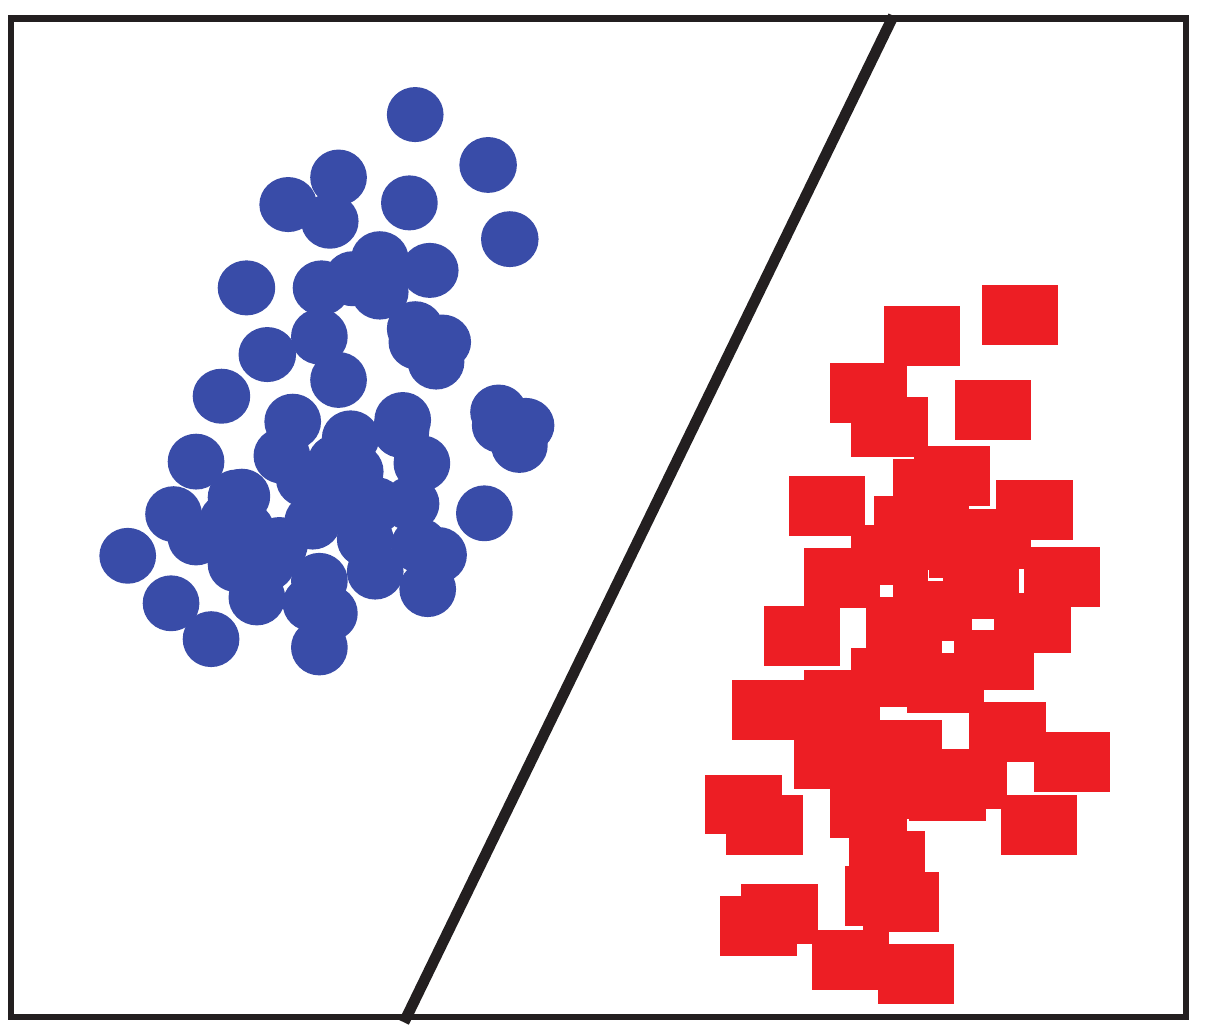
\includegraphics[scale=0.5]{./figures/fig-distribution-source.pdf}
		\label{fig-distribution-source}}
	~\vline
	~
	\subfigure[目标域数据: 类型I]{
		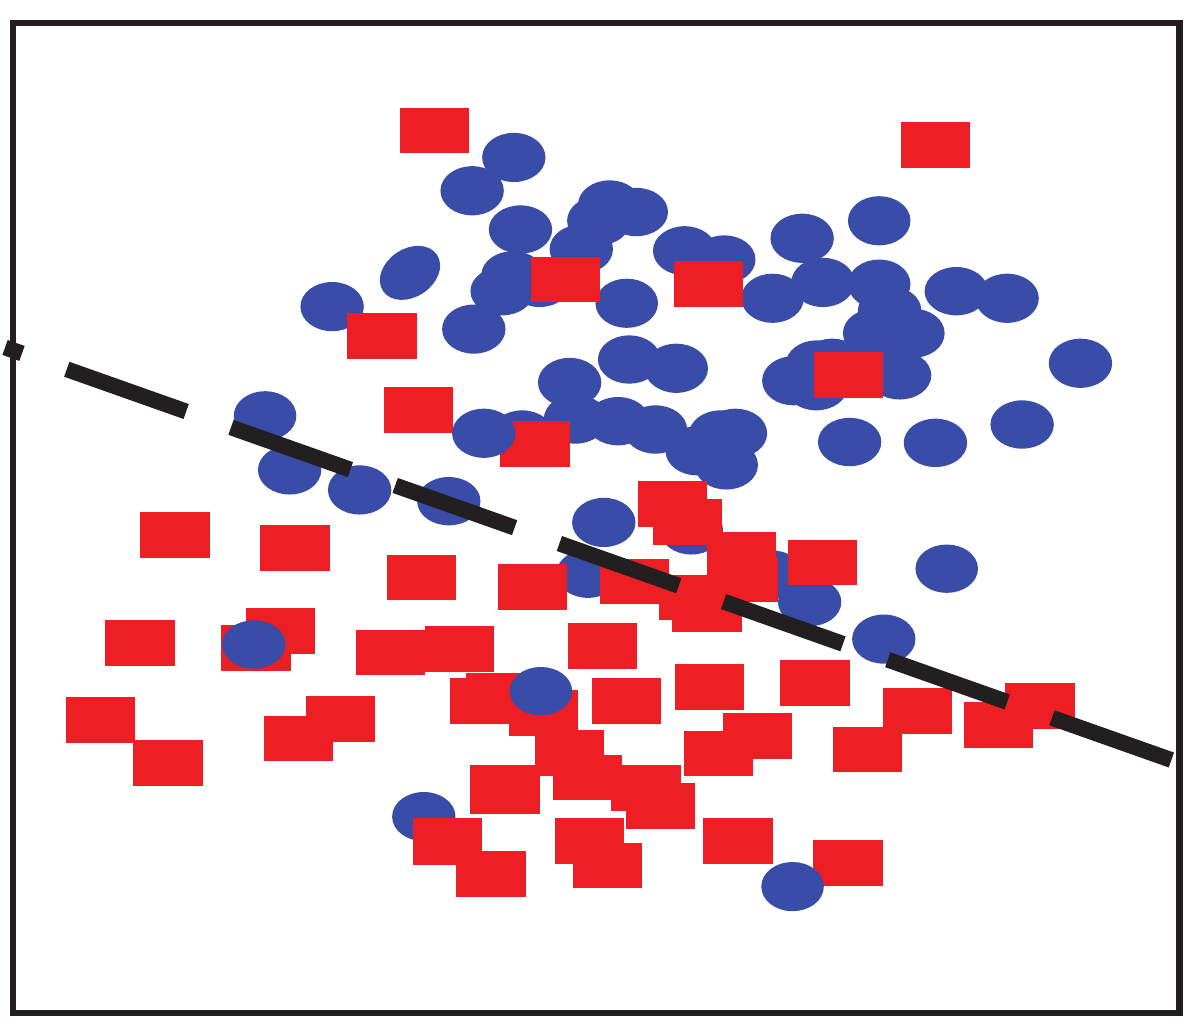
\includegraphics[scale=0.5]{./figures/fig-distribution-target1.pdf}
		\label{fig-distribution-target1}}
	~
	\subfigure[目标域数据:类型II]{
		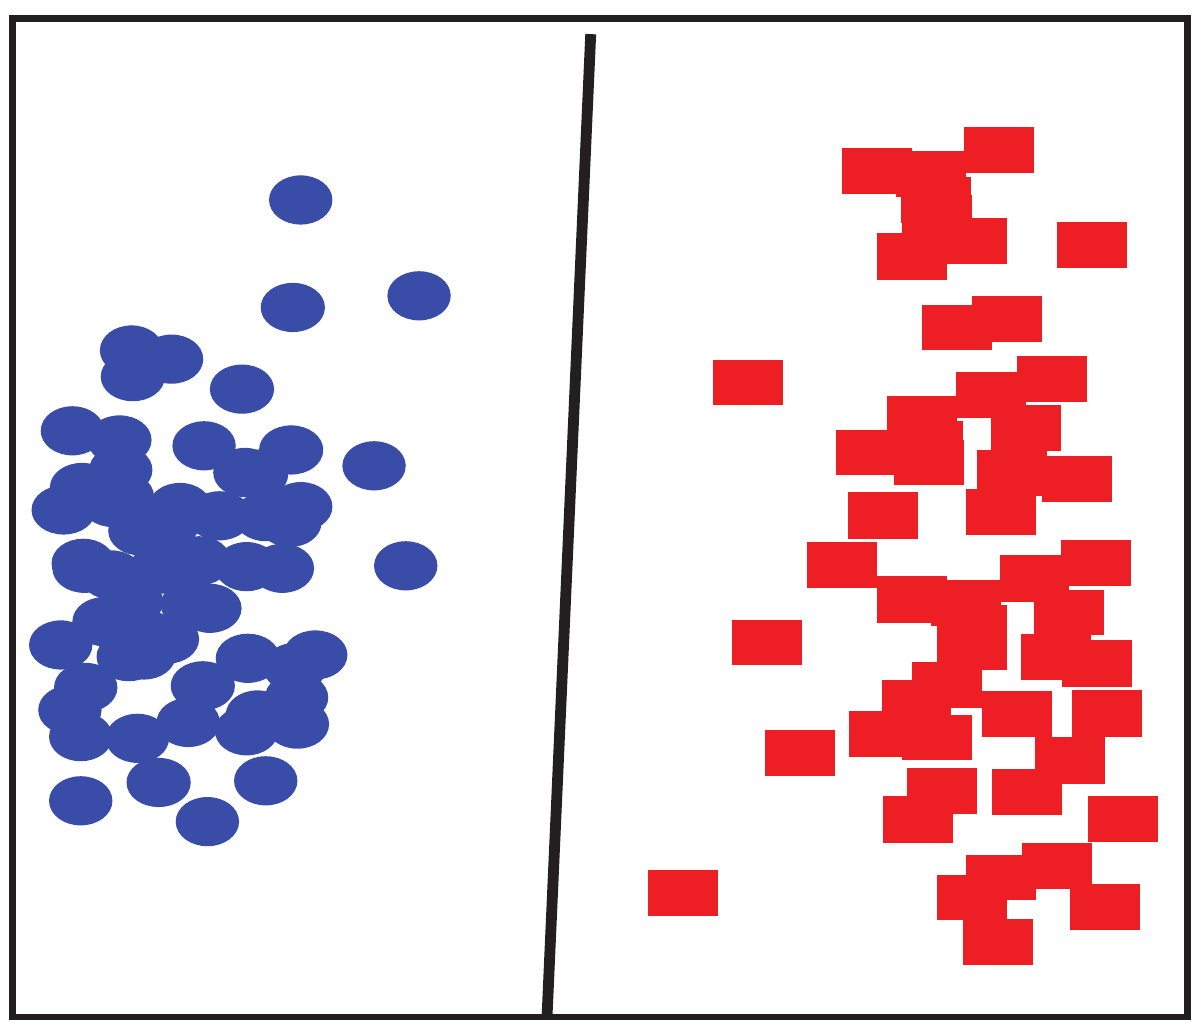
\includegraphics[scale=0.5]{./figures/fig-distribution-target2.pdf}
		\label{fig-distribution-target2}}
	\caption{不同数据分布的目标域数据}
	\label{fig-distribution}
\end{figure}

根据数据分布的性质,这类方法又可以分为\textit{边缘分布自适应、条件分布自适应}、以及\textit{联合分布自适应}。下面我们分别介绍每类方法的基本原理和代表性研究工作。介绍每类研究工作时,我们首先给出基本思路,然后介绍该类方法的核心,最后结合最近的相关工作介绍该类方法的扩展。

\subsection{边缘分布自适应}

\subsubsection{基本思路}

边缘分布自适应方法(Marginal Distribution Adaptation)的目标是减小源域和目标域的边缘概率分布的距离,从而完成迁移学习。从形式上来说,边缘分布自适应方法是用$P(\mathbf{x}_s)$和$P(\mathbf{x}_t)$之间的距离来近似两个领域之间的差异。即:

\begin{equation}
	\label{eq-marginal-general}
	DISTANCE(\mathcal{D}_s,\mathcal{D}_t) \approx ||P(\mathbf{x}_s) - P(\mathbf{x}_t)||
\end{equation}

边缘分布自适应对应于图~\ref{fig-distribution}中由图~\ref{fig-distribution-source}迁移到图~\ref{fig-distribution-target1}的情形。

\subsubsection{核心方法}

边缘分布自适应的方法最早由香港科技大学杨强教授团队提出~\cite{pan2011domain},方法名称为迁移成分分析(Transfer Component Analysis)。由于$P(\mathbf{x}_s) \ne P(\mathbf{x}_t)$,因此,直接减小二者之间的距离是不可行的。TCA假设存在一个特征映射$\phi$,使得映射后数据的分布$P(\phi(\mathbf{x}_s)) \approx P(\phi(\mathbf{x}_t))$。TCA假设如果边缘分布接近,那么两个领域的条件分布也会接近,即条件分布$P(y_s | \phi(\mathbf{x}_s))) \approx P(y_t | \phi(\mathbf{x}_t)))$。这就是TCA的全部思想。因此,我们现在的目标是,找到这个合适的$\phi$。

但是世界上有无穷个这样的$\phi$,也许终我们一生也无法找到合适的那一个。庄子说过,吾生也有涯,而知也无涯,以有涯随无涯,殆已!我们肯定不能通过穷举的方法来找$\phi$的。那么怎么办呢?

回到迁移学习的本质上来:最小化源域和目标域的距离。好了,我们能不能先假设这个$\phi$是已知的,然后去求距离,看看能推出什么呢?

更进一步,这个距离怎么算?机器学习中有很多种形式的距离,从欧氏距离到马氏距离,从曼哈顿距离到余弦相似度,我们需要什么距离呢?TCA利用了一个经典的也算是比较“高端”的距离叫做最大均值差异(MMD,maximum mean discrepancy)。我们令$n_1,n_2$分别表示源域和目标域的样本个数,那么它们之间的MMD距离可以计算为:

\begin{equation}
	\label{eq-distribution-mmd}
	DISTANCE(\mathbf{x}_{s},\mathbf{x}_{t})= \begin{Vmatrix} \frac{1}{n_1} \sum \limits_{i=1}^{n_1} \phi(\mathbf{x}_{i}) - \frac{1}{n_2}\sum \limits _{j=1}^{n_2} \phi(\mathbf{x}_{j}) \end{Vmatrix}_{\mathcal{H}}
\end{equation}

MMD是做了一件什么事呢?简单,就是求映射后源域和目标域的\textit{均值之差}。

事情到这里似乎也没什么进展:我们想求的$\phi$仍然没法求。

TCA是怎么做的呢,这里就要感谢矩阵了!我们发现,上面这个MMD距离平方展开后,有二次项乘积的部分!那么,联系在SVM中学过的核函数,把一个难求的映射以核函数的形式来求,不就可以了?于是,TCA引入了一个核矩阵$\mathbf{K}$:

\begin{equation}
	\mathbf{K}=\begin{bmatrix}\mathbf{K}_{s,s} & \mathbf{K}_{s,t}\\\mathbf{K}_{t,s} & \mathbf{K}_{t,t}\end{bmatrix} 
\end{equation}

以及一个MMD矩阵$\mathbf{L}$,它的每个元素的计算方式为:

\begin{equation}
	l_{ij}=\begin{cases} \frac{1}{{n_1}^2} & \mathbf{x}_i,\mathbf{x}_j \in \mathcal{D}_s,\\ \frac{1}{{n_2}^2} & \mathbf{x}_i,\mathbf{x}_j \in \mathcal{D}_t,\\ -\frac{1}{n_1 n_2} & \text{otherwise} \end{cases}
\end{equation}

这样的好处是,直接把那个难求的距离,变换成了下面的形式:

\begin{equation}
	\mathrm{tr}(\mathbf{KL})-\lambda \mathrm{tr}(\mathbf{K})
\end{equation}

其中,$\mathrm{tr}(\cdot)$操作表示求矩阵的迹,用人话来说就是一个矩阵对角线元素的和。这样是不是感觉离目标又进了一步呢?

其实这个问题到这里就已经是可解的了,也就是说,属于计算机的部分已经做完了。只不过它是一个数学中的半定规划(SDP,semi-definite programming)的问题,解决起来非常耗费时间。由于TCA的第一作者Sinno Jialin Pan以前是中山大学的数学硕士,他想用更简单的方法来解决。他是怎么做的呢?

他想出了用降维的方法去构造结果。用一个更低维度的矩阵$\mathbf{W}$:
\begin{equation}
	\widetilde{\mathbf{K}}=({\mathbf{K}}{\mathbf{K}}^{-1/2}\widetilde{\mathbf{W}})(\widetilde{\mathbf{W}}^{\top}{\mathbf{K}}^{-1/2}{\mathbf{K}})={\mathbf{K}}\mathbf{W} \mathbf{W}^{\top}{\mathbf{K}}
\end{equation}

这里的$\mathbf{W}$矩阵是比$\mathbf{K}$更低维度的矩阵。最后的$\mathbf{W}$就是问题的解答了!

好了,问题到这里,整理一下,TCA最后的优化目标是:

\begin{equation}
	\begin{split} \min_\mathbf{W} \quad& \mathrm{tr}(\mathbf{W}^\top \mathbf{K} \mathbf{L} \mathbf{K} \mathbf{W}) + \mu \mathrm{tr}(\mathbf{W}^\top \mathbf{W})\\ \text{s.t.} \quad & \mathbf{W}^\top \mathbf{K} \mathbf{H} \mathbf{K} \mathbf{W} = \mathbf{I}_m \end{split} 
\end{equation}

这里的$\mathbf{H}$是一个中心矩阵,$\mathbf{H} = \mathbf{I}_{n_1 + n_2} - 1/(n_1 + n_2)\mathbf{11}^\top$.

这个式子下面的条件是什么意思呢?那个$\min$的目标我们大概理解,就是要最小化源域和目标域的距离,加上$\mathbf{W}$的约束让它不能太复杂。那么下面的条件是什么呢?下面的条件就是要实现第二个目标:维持各自的数据特征。

TCA要维持的是什么特征呢?文章中说是variance,但是实际是scatter matrix,就是数据的散度。就是说,一个矩阵散度怎么计算?对于一个矩阵$\mathbf{A}$,它的scatter matrix就是$\mathbf{A} \mathbf{H} \mathbf{A}^\top$。这个$\mathbf{H}$就是上面的中心矩阵啦。

解决上面的优化问题时,作者又求了它的拉格朗日对偶。最后得出结论,$\mathbf{W}$的解就是它的前$m$个特征值!简单不?数学美不美?

好了,我们现在总结一下TCA方法的步骤。输入是两个特征矩阵,我们首先计算$\mathbf{L}$和$\mathbf{H}$矩阵,然后选择一些常用的核函数进行映射(比如线性核、高斯核)计算$\mathbf{K}$,接着求$({\mathbf{K}} \mathbf{L} {\mathbf{K}}+\mu \mathbf{I})^{-1}{\mathbf{K}} \mathbf{H}{\mathbf{K}}$的前$m$个特征值。仅此而已。然后,得到的就是源域和目标域的降维后的数据,我们就可以在上面用传统机器学习方法了。

为了形象地展示TCA方法的优势,我们借用~\cite{pan2011domain}中提供的可视化效果,在图中展示了对于源域和目标域数据(红色和蓝色),分别由PCA(主成分分析)和TCA得到的分布结果。从图~\ref{fig-distribution-tca}中可以很明显地看出,对于概率分布不同的两部分数据,在经过TCA处理后,概率分布更加接近。这说明了TCA在拉近数据分布距离上的优势。

\begin{figure}[htbp]
	\centering
	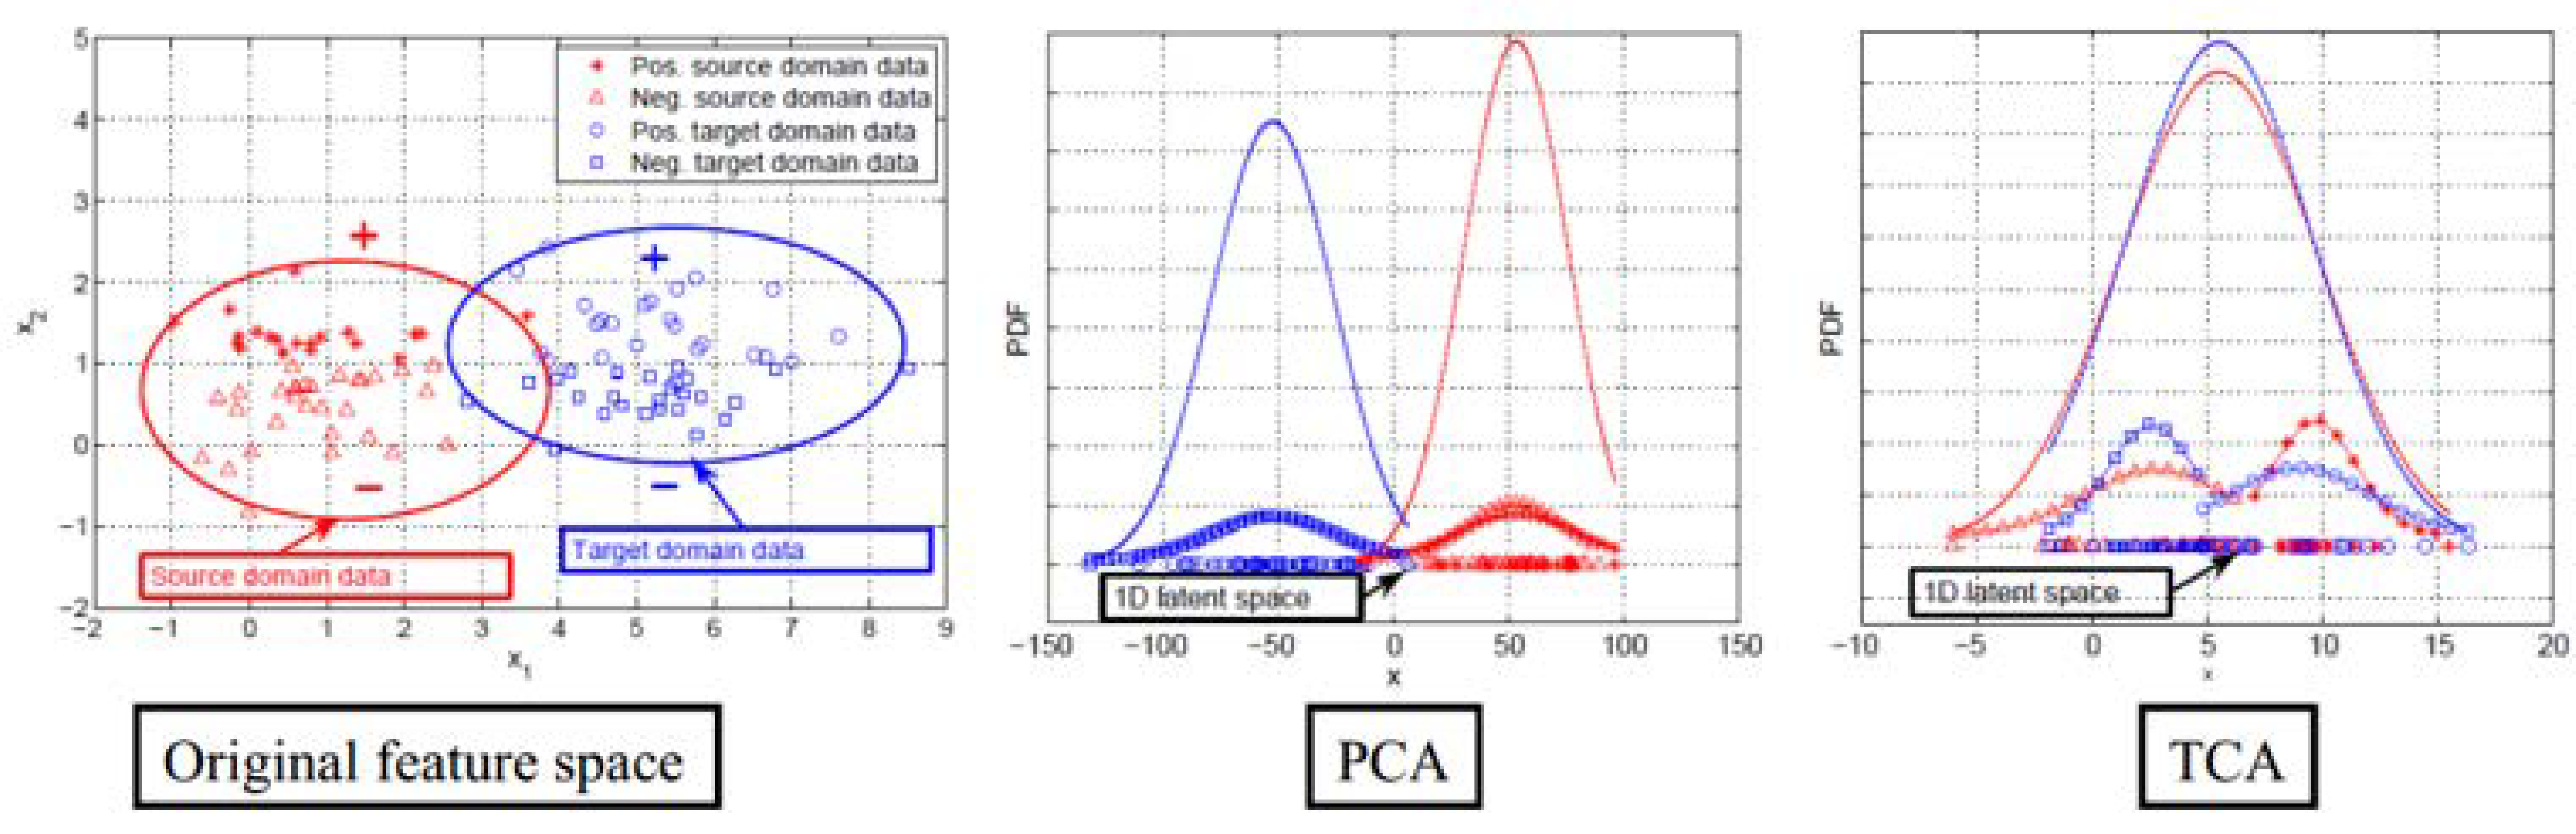
\includegraphics[scale=0.6]{./figures/fig-distribution-tca.pdf}
	\caption{TCA和PCA的效果对比}
	\label{fig-distribution-tca}
\end{figure}

\subsubsection{扩展}

TCA方法是迁移学习领域一个经典的方法,之后的许多研究工作都以TCA为基础。我们列举部分如下:

\begin{itemize}
	\item ACA (Adapting Component Analysis)~\cite{dorri2012adapting}: 在TCA中加入HSIC
	\item DTMKL (Domain Transfer Multiple Kernel Learning)~\cite{duan2012domain}: 在TCA中加入了MK-MMD,用了新的求解方式
	\item TJM (Transfer Joint Matching)~\cite{long2014transfer}: 在优化目标中同时进行边缘分布自适应和源域样本选择
	\item DDC (Deep Domain Confusion)~\cite{tzeng2014deep}: 将MMD度量加入了深度网络特征层的loss中(我们将会在深度迁移学习中介绍此工作)
	\item DAN (Deep Adaptation Network)~\cite{long2015learning}: 扩展了DDC的工作,将MMD换成了MK-MMD,并且进行多层loss计算(我们将会在深度迁移学习中介绍此工作)
	\item DME (Distribution Matching Embedding): 先计算变换矩阵,再进行特征映射(与TCA顺序相反)
	\item CMD (Central Moment Matching)~\cite{zellinger2017central}: MMD着眼于一阶,此工作将MMD推广到了多阶
\end{itemize}

\subsection{条件分布自适应}

条件分布自适应方法(Conditional Distribution Adaptation)的目标是减小源域和目标域的条件概率分布的距离,从而完成迁移学习。从形式上来说,条件分布自适应方法是用$P(y_s|\mathbf{x}_s)$和$P(y_t|\mathbf{x}_t)$之间的距离来近似两个领域之间的差异。即:

\begin{equation}
\label{eq-conditional-general}
DISTANCE(\mathcal{D}_s,\mathcal{D}_t) \approx ||P(y_s|\mathbf{x}_s) - P(y_t|\mathbf{x}_t)||
\end{equation}

条件分布自适应对应于图~\ref{fig-distribution}中由图~\ref{fig-distribution-source}迁移到图~\ref{fig-distribution-target2}的情形。

目前单独利用条件分布自适应的工作较少,这些工作主要可以在~\cite{saito2017asymmetric}中找到。最近,中科院计算所的Wang等人提出了STL方法(Stratified Transfer Learning)~\cite{wang2018stratified}。作者提出了\textit{类内迁移}(Intra-class Transfer)的思想。指出现有的绝大多数方法都只是学习一个全局的特征变换(Global Domain Shift),而忽略了类内的相似性。类内迁移可以利用类内特征,实现更好的迁移效果。

STL方法的基本思路如图~\ref{fig-distribution-stl}所示。首先利用大多数投票的思想,对无标定的位置行为生成伪标签;然后在再生核希尔伯特空间中,利用类内相关性进行自适应地空间降维,使得不同情境中的行为数据之间的相关性增大;最后,通过二次标定,实现对未知标定数据的精准标定。

\begin{figure}[htbp]
	\centering
	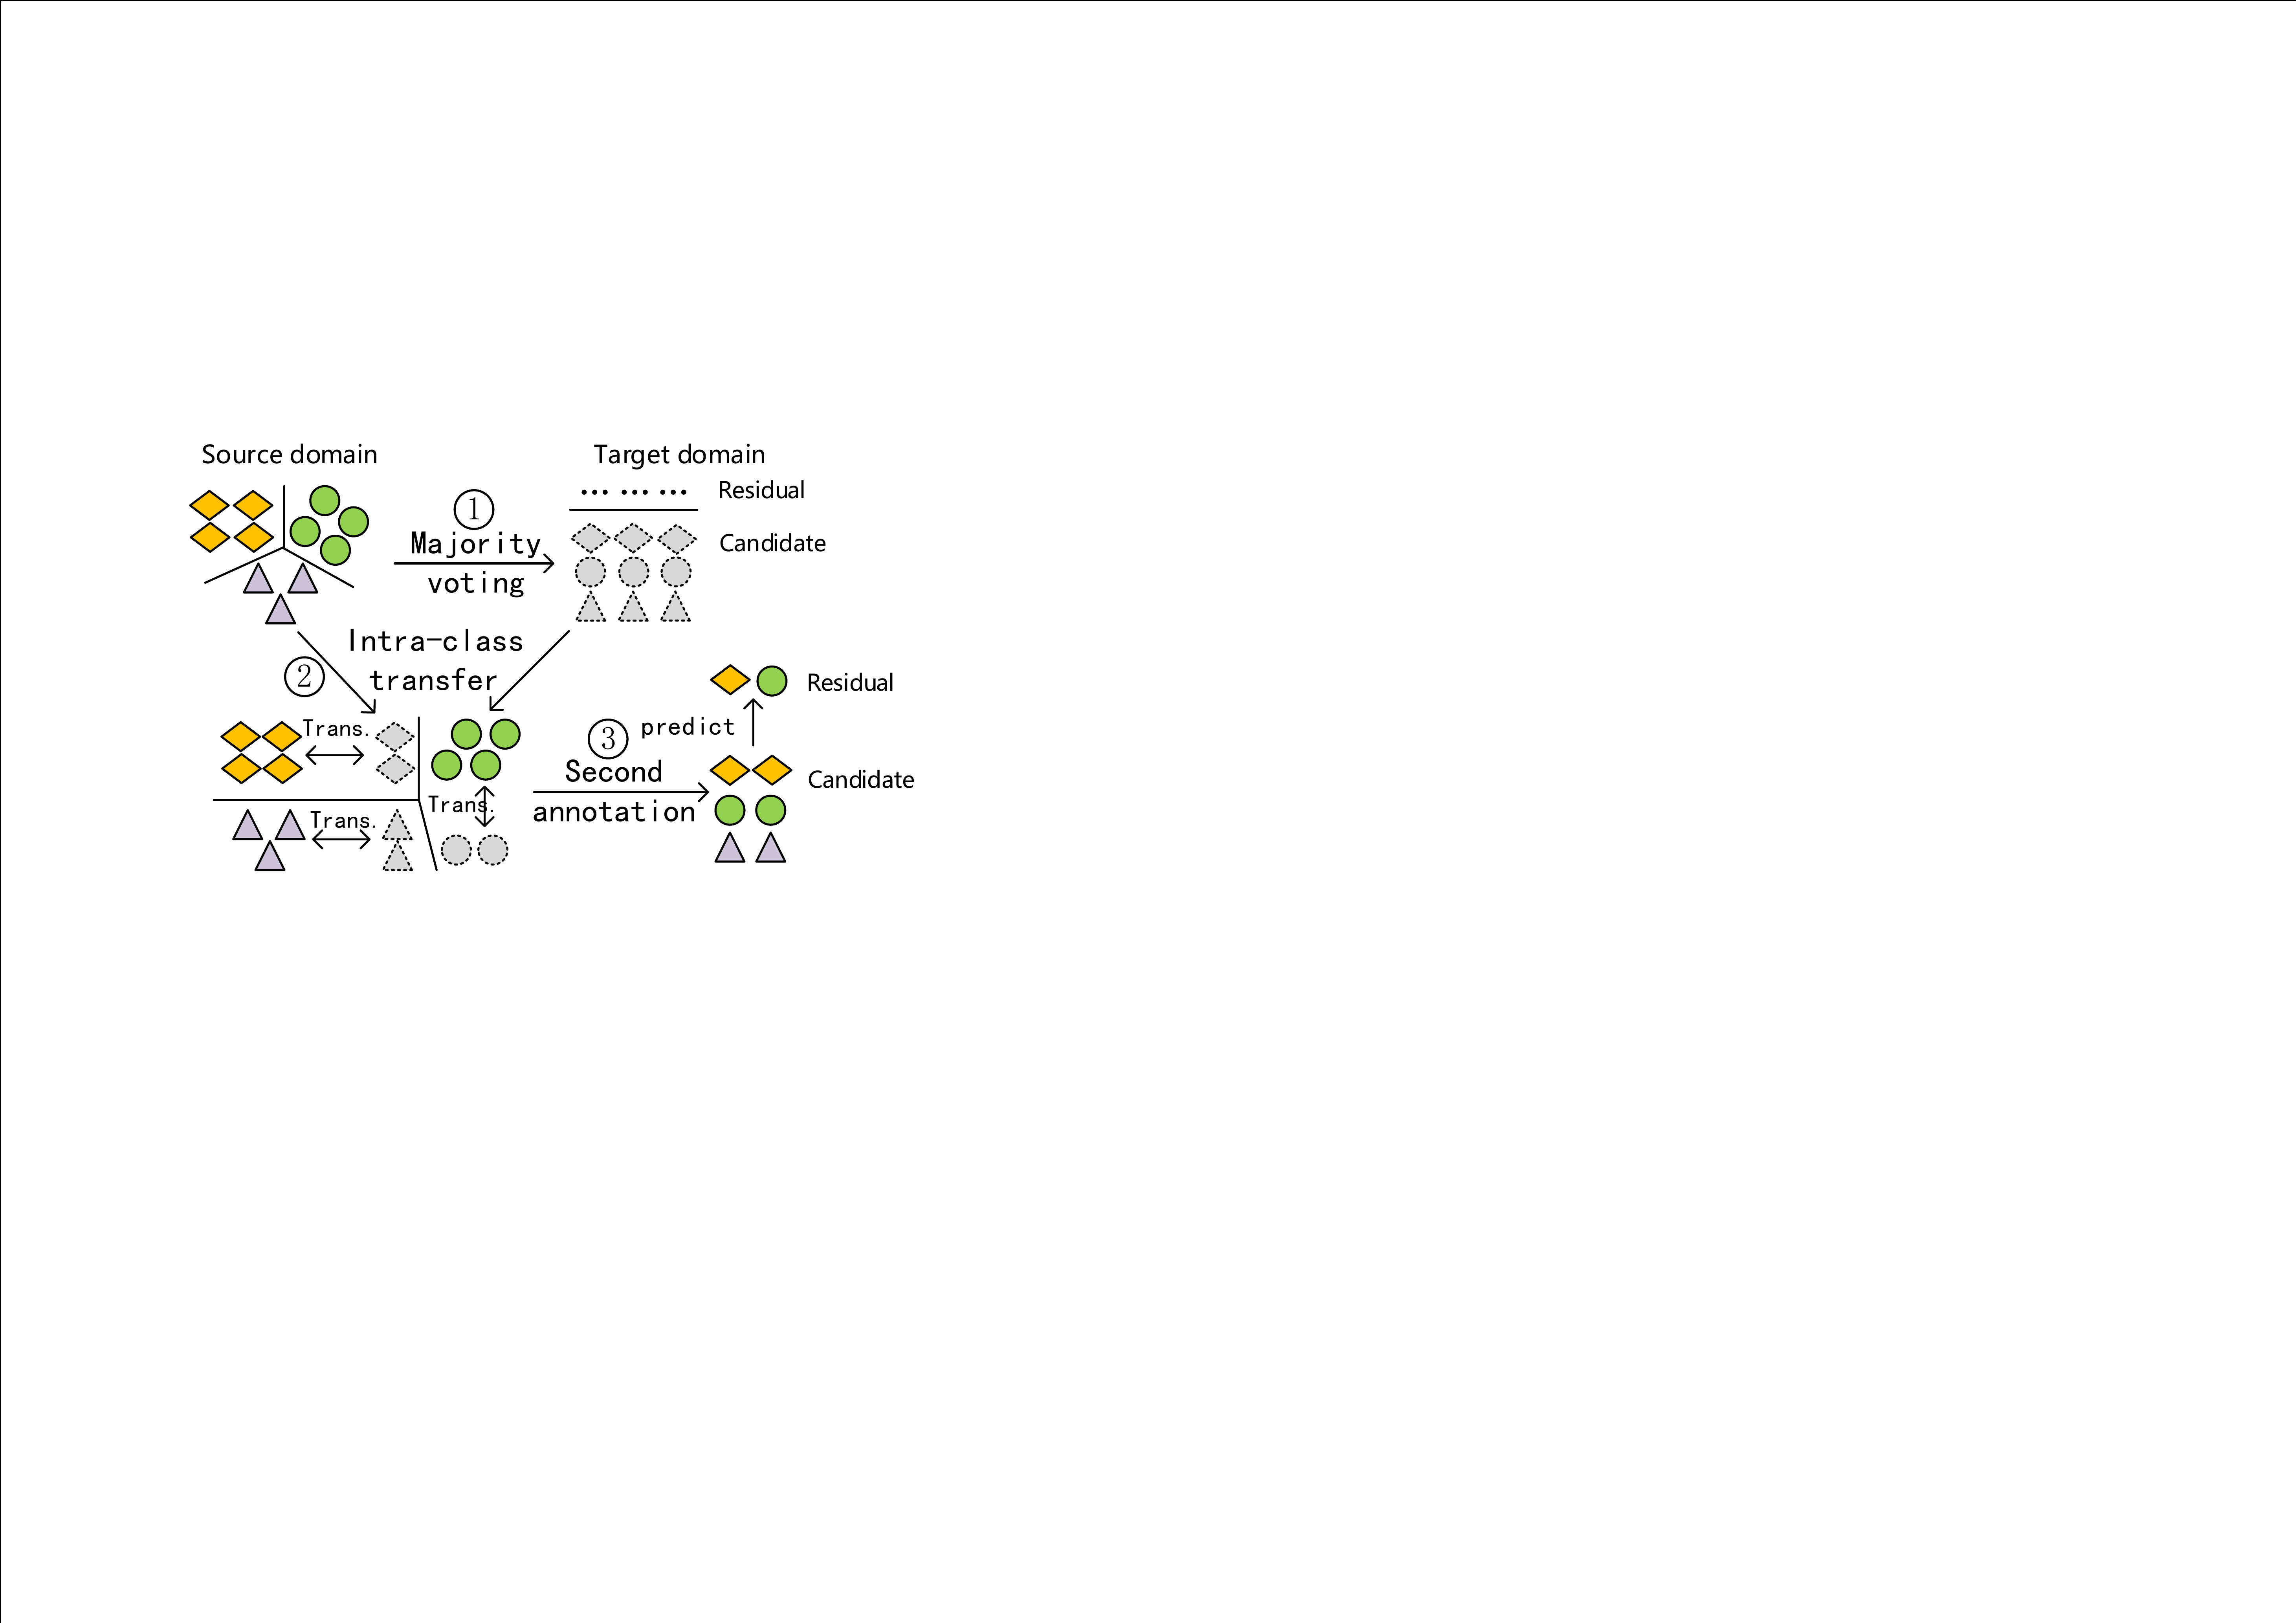
\includegraphics[scale=0.85]{./figures/fig-distribution-stl.pdf}
	\caption{STL方法的示意图}
	\label{fig-distribution-stl}
\end{figure}

为了实现\textit{类内迁移},我们需要计算每一类别的MMD距离。由于目标域没有标记,作者使用来自大多数投票结果中的伪标记。更加准确地说,用$c \in \{1, 2, \cdots, C\}$来表示类别标记,则类内迁移可以按如下方式计算:

\begin{equation}
\label{equ-stl-stra}
D(\mathcal{D}_{s},\mathcal{D}_{t})
=\sum_{c=1}^{C}\left \Vert \frac{1}{n^{(c)}_1} \sum_{\mathbf{x}_i \in \mathcal{D}^{(c)}_s} \phi(\mathbf{x}_i) - \frac{1}{n^{(c)}_2} \sum_{\mathbf{x}_j \in \mathcal{D}^{(c)}_t} \phi(\mathbf{x}_j) \right \Vert ^2_\mathcal{H}
\end{equation}

其中,$\mathcal{D}^{(c)}_s$和$\mathcal{D}^{(c)}_t$分别表示源域和目标域中属于类别$c$的样本。$n^{(c)}_1=|\mathcal{D}^{(c)}_s|$,且$n^{(c)}_2=|\mathcal{D}_t|$。

接下来的步骤请参照STL方法原文进行理解。

STL方法在大量行为识别数据中进行了跨位置行为识别的实验。实验结果表明,该方法可以很好地实现跨领域的行为识别任务,取得了当前最好的效果。

\subsection{联合分布自适应}

\subsubsection{基本思路}

联合分布自适应方法(Joint Distribution Adaptation)的目标是减小源域和目标域的联合概率分布的距离,从而完成迁移学习。从形式上来说,联合分布自适应方法是用$P(\mathbf{x}_s)$和$P(\mathbf{x}_t)$之间的距离、以及$P(y_s|\mathbf{x}_s)$和$P(y_t|\mathbf{x}_t)$之间的距离来近似两个领域之间的差异。即:

\begin{equation}
\label{eq-joint-general}
DISTANCE(\mathcal{D}_s,\mathcal{D}_t) \approx ||P(\mathbf{x}_s) - P(\mathbf{x}_t)|| + ||P(y_s|\mathbf{x}_s) - P(y_t|\mathbf{x}_t)||
\end{equation}

联合分布自适应对应于图~\ref{fig-distribution}中由图~\ref{fig-distribution-source}迁移到图~\ref{fig-distribution-target1}的情形、以及图~\ref{fig-distribution-source}迁移到图~\ref{fig-distribution-target2}的情形。

\subsubsection{核心方法}

联合分布适配的JDA方法~\cite{long2013transfer}首次发表于2013年的ICCV(计算机视觉领域顶会,与CVPR类似),它的作者是当时清华大学的博士生(现为清华大学助理教授)龙明盛。

假设是最基本的出发点。那么JDA这个方法的假设是什么呢?就是假设两点:1)源域和目标域边缘分布不同,2)源域和目标域条件分布不同。既然有了目标,同时适配两个分布不就可以了吗?于是作者很自然地提出了联合分布适配方法:适配联合概率。

不过这里我感觉有一些争议:边缘分布和条件分布不同,与联合分布不同并不等价。所以这里的“联合”二字实在是会引起歧义。我的理解是,同时适配两个分布,也可以叫联合,而不是概率上的“联合”。尽管作者在文章里第一个公式就写的是适配联合概率,但是这里感觉是有一些问题的。我们抛开它这个有歧义的,把“联合”理解成同时适配两个分布。

那么,JDA方法的目标就是,寻找一个变换$\mathbf{A}$,使得经过变换后的$P(\mathbf{A}^\top \mathbf{x}_s)$和$P(\mathbf{A}^\top \mathbf{x}_t)$的距离能够尽可能地接近,同时,$P(y_s|\mathbf{A}^\top \mathbf{x}_s)$和$P(y_t|\mathbf{A}^\top \mathbf{x}_t)$的距离也要小。很自然地,这个方法也就分成了两个步骤。

\textit{边缘分布适配}

首先来适配边缘分布,也就是$P(\mathbf{A}^\top \mathbf{x}_s)$和$P(\mathbf{A}^\top \mathbf{x}_t)$的距离能够尽可能地接近。其实这个操作就是迁移成分分析(TCA)。我们仍然使用MMD距离来最小化源域和目标域的最大均值差异。MMD距离是

\begin{equation}
	\left \Vert \frac{1}{n} \sum_{i=1}^{n} \mathbf{A}^\top \mathbf{x}_{i} - \frac{1}{m} \sum_{j=1}^{m} \mathbf{A}^\top \mathbf{x}_{j} \right \Vert ^2_\mathcal{H}
\end{equation}

这个式子实在不好求解。我们引入核方法,化简这个式子,它就变成了

\begin{equation}
	D(\mathcal{D}_s,\mathcal{D}_t)=tr(\mathbf{A}^\top \mathbf{X} \mathbf{M}_0 \mathbf{X}^\top \mathbf{A})
\end{equation}

其中$\mathbf{A}$就是变换矩阵,我们把它加黑加粗,$\mathbf{X}$是源域和目标域合并起来的数据。$\mathbf{M}_0$是一个MMD矩阵:

\begin{equation}
	(\mathbf{M}_0)_{ij}=\begin{cases} \frac{1}{n^2}, & \mathbf{x}_i,\mathbf{x}_j \in \mathcal{D}_s\\ \frac{1}{m^2}, & \mathbf{x}_i,\mathbf{x}_j \in \mathcal{D}_t\\ -\frac{1}{mn}, & \text{otherwise} \end{cases}
\end{equation}

$n,m$分别是源域和目标域样本的个数。

到此为止没有什么创新点,因为这就是一个TCA。

\textit{条件分布适配}

这是我们要做的第二个目标,适配源域和目标域的条件概率分布。也就是说,还是要找一个变换$\mathbf{A}$,使得$P(y_s|\mathbf{A}^\top \mathbf{x}_s)$和$P(y_t|\mathbf{A}^\top \mathbf{x}_t)$的距离也要小。那么简单了,我们再用一遍MMD啊。可是问题来了:我们的目标域里,没有$y_t$,没法求目标域的条件分布!

这条路看来是走不通了。也就是说,直接建模$P(y_t|\mathbf{x}_t)$不行。那么,能不能有别的办法可以逼近这个条件概率?我们可以换个角度,利用类条件概率$P(\mathbf{x}_t|y_t)$。根据贝叶斯公式$P(y_t|\mathbf{x}_t)=p(y_t)p(\mathbf{x}_t|y_t)$,我们如果忽略$P(\mathbf{x}_t)$,那么岂不是就可以用$P(\mathbf{x}_t|y_t)$来近似$P(y_t|\mathbf{x}_t)$?

而这样的近似也不是空穴来风。在统计学上,有一个概念叫做\textit{充分统计量},它是什么意思呢?大概意思就是说,如果样本里有太多的东西未知,样本足够好,我们就能够从中选择一些统计量,近似地代替我们要估计的分布。好了,我们为近似找到了理论依据。

实际怎么做呢?我们依然没有$y_t$。采用的方法是,用$(\mathbf{x}_s,y_s)$来训练一个简单的分类器(比如knn、逻辑斯特回归),到$\mathbf{x}_t$上直接进行预测。总能够得到一些伪标签$\hat{y}_t$。我们根据伪标签来计算,这个问题就可解了。

类与类之间的MMD距离表示为

\begin{equation}
	\sum_{c=1}^{C}\left \Vert \frac{1}{n_c} \sum_{\mathbf{x}_{i} \in \mathcal{D}^{(c)}_s} \mathbf{A}^\top \mathbf{x}_{i} - \frac{1}{m_c} \sum_{\mathbf{x}_{i} \in \mathcal{D}^{(c)}_t} \mathbf{A}^\top \mathbf{x}_{i} \right \Vert ^2_\mathcal{H}
\end{equation}

其中,$n_c,m_c$分别标识源域和目标域中来自第$c$类的样本个数。同样地我们用核方法,得到了下面的式子

\begin{equation}
	\sum_{c=1}^{C}tr(\mathbf{A}^\top \mathbf{X} \mathbf{M}_c \mathbf{X}^\top \mathbf{A})
\end{equation}

其中$\mathbf{M}_c$为

\begin{equation}
	(\mathbf{M}_c)_{ij}=\begin{cases} \frac{1}{n^2_c}, & \mathbf{x}_i,\mathbf{x}_j \in \mathcal{D}^{(c)}_s\\ \frac{1}{m^2_c}, & \mathbf{x}_i,\mathbf{x}_j \in \mathcal{D}^{(c)}_t\\ -\frac{1}{m_c n_c}, & \begin{cases} \mathbf{x}_i \in \mathcal{D}^{(c)}_s ,\mathbf{x}_j \in \mathcal{D}^{(c)}_t \\ \mathbf{x}_i \in \mathcal{D}^{(c)}_t ,\mathbf{x}_j \in \mathcal{D}^{(c)}_s \end{cases}\\ 0, & \text{otherwise}\end{cases}
\end{equation}

现在我们把两个距离结合起来,得到了一个总的优化目标:

\begin{equation}
	\min \sum_{c=0}^{C}tr(\mathbf{A}^\top \mathbf{X} \mathbf{M}_c \mathbf{X}^\top \mathbf{A}) + \lambda \Vert \mathbf{A} \Vert ^2_F
\end{equation}

看到没,通过$c=0 \cdots C$就把两个距离统一起来了!其中的$\lambda \Vert \mathbf{A} \Vert ^2_F$是正则项,使得模型是\textit{良好定义}(Well-defined)的。

我们还缺一个限制条件,不然这个问题无法解。限制条件是什么呢?和TCA一样,变换前后数据的方差要维持不变。怎么求数据的方差呢,还和TCA一样:$\mathbf{A}^\top \mathbf{X} \mathbf{H} \mathbf{X}^\top \mathbf{A} = \mathbf{I}$,其中的$\mathbf{H}$也是中心矩阵,$\mathbf{I}$是单位矩阵。也就是说,我们又添加了一个优化目标是要$\max \mathbf{A}^\top \mathbf{X} \mathbf{H} \mathbf{X}^\top \mathbf{A}$(这一个步骤等价于PCA了)。和原来的优化目标合并,优化目标统一为:

\begin{equation}
	\min \frac{\sum_{c=0}^{C}tr(\mathbf{A}^\top \mathbf{X} \mathbf{M}_c \mathbf{X}^\top \mathbf{A}) + \lambda \Vert \mathbf{A}\Vert^2_F}{ \mathbf{A}^\top \mathbf{X} \mathbf{H} \mathbf{X}^\top \mathbf{A}}
\end{equation}

这个式子实在不好求解。但是,有个东西叫做Rayleigh quotient~\footnote{\url{https://www.wikiwand.com/en/Rayleigh_quotient}},上面两个一样的这种形式。因为$\mathbf{A}$是可以进行拉伸而不改变最终结果的,而如果下面为0的话,整个式子就求不出来值了。所以,我们直接就可以让下面不变,只求上面。所以我们最终的优化问题形式搞成了

\begin{equation}
	\min \quad \sum_{c=0}^{C}tr(\mathbf{A}^\top \mathbf{X} \mathbf{M}_c \mathbf{X}^\top \mathbf{A}) + \lambda \Vert \mathbf{A} \Vert ^2_F \quad \text{s.t.} \quad \mathbf{A}^\top \mathbf{X} \mathbf{H} \mathbf{X}^\top \mathbf{A} = \mathbf{I}
\end{equation}

怎么解?太简单了,可以用拉格朗日法。最后变成了

\begin{equation}
	\left(\mathbf{X} \sum_{c=0}^{C} \mathbf{M}_c \mathbf{X}^\top + \lambda \mathbf{I}\right) \mathbf{A} =\mathbf{X} \mathbf{H} \mathbf{X}^\top \mathbf{A} \Phi 
\end{equation}

其中的$\Phi$是拉格朗日乘子。别看这个东西复杂,又有要求解的$\mathbf{A}$,又有一个新加入的$\Phi$ 。但是它在Matlab里是可以直接解的(用$\mathrm{eigs}$函数即可)。这样我们就得到了变换$\mathbf{A}$,问题解决了。

可是伪标签终究是伪标签啊,肯定精度不高,怎么办?有个东西叫做\textit{迭代},一次不行,我们再做一次。后一次做的时候,我们用上一轮得到的标签来作伪标签。这样的目的是得到越来越好的伪标签,而参与迁移的数据是不会变的。这样往返多次,结果就自然而然好了。

JDA方法是十分经典的迁移学习方法。后续的相关工作通过在JDA的基础上加入额外的损失项,使得迁移学习的效果得到了很大提升。我们在这里简要介绍一些基于JDA的相关工作。

\begin{itemize}
	\item ARTL~(Adaptation Regularization)~\cite{long2014adaptation}: 将JDA嵌入一个结构风险最小化框架中,用表示定理直接学习分类器
	\item VDA~\cite{tahmoresnezhad2016visual}: 在JDA的优化目标中加入了类内距和类间距的计算
	\item \cite{hsiao2016learning}: 在JDA的基础上加入结构不变性控制
	\item \cite{hou2015unsupervised}: 在JDA的基础上加入目标域的选择
	\item JGSA~(Joint Geometrical and Statistical Alignment)~\cite{zhang2017joint}: 在JDA的基础上加入类内距、类间距、标签持久化
	\item JAN~(Joint Adaptation Network)~\cite{long2017deep}: 提出了联合分布度量JMMD,在深度网络中进行联合分布的优化
\end{itemize}

\subsection{动态分布自适应}

\textbf{平衡分布自适应BDA}

在最近的研究中,来自中科院计算所的Wang等人~\cite{wang2017balanced}注意到了JDA的不足:\textit{边缘分布自适应和条件分布自适应并不是同等重要}。回到图~\ref{fig-distribution}表示的两种分布的问题上来。显然,当目标域是图~\ref{fig-distribution-target1}所示的情况时,边缘分布应该被优先考虑;而当目标域是图~\ref{fig-distribution-target2}所示的情况时,条件分布应该被优先考虑。JDA以及后来的扩展工作均忽视了这一问题。

作者提出了BDA方法(Balanced Distribution Adaptation)来解决这一问题。该方法能够根据特定的数据领域,自适应地调整分布适配过程中边缘分布和条件分布的重要性。准确而言,BDA通过采用一种\textit{平衡因子}$\mu$来动态调整两个分布之间的距离
\begin{equation}
\label{equ-mummd}
\begin{split}
DISTANCE(\mathcal{D}_s,\mathcal{D}_t) \approx  (1 &- \mu)DISTANCE(P(\mathbf{x}_s),P(\mathbf{x}_t))\\
&+ \mu DISTANCE(P(y_s|\mathbf{x}_s),P(y_t|\mathbf{x}_t))
\end{split}
\end{equation}
其中$\mu \in [0,1]$表示平衡因子。当$\mu \rightarrow 0$,这表示源域和目标域数据本身存在较大的差异性,因此,边缘分布适配更重要;当$\mu \rightarrow 1$时,这表示源域和目标域数据集有较高的相似性,因此,条件概率分布适配更加重要。综合上面的分析可知,平衡因子可以根据实际数据分布的情况,动态地调节每个分布的重要性,并取得良好的分布适配效果。

其中的平衡因子$\mu$可以通过分别计算两个领域数据的整体和局部的$\mathcal{A}$-distance近似给出。特别地,当$\mu = 0$时,方法退化为TCA;当$\mu = 0.5$时,方法退化为JDA。

我们采用BDA文章中的图来具体地展示出$\mu$的作用。图~\ref{fig-distribution-bda}的结果清晰地显示出,平衡因子可以取得比JDA、TCA更小的MMD距离、更高的精度。

%\begin{figure}[htbp]
%	\centering
%	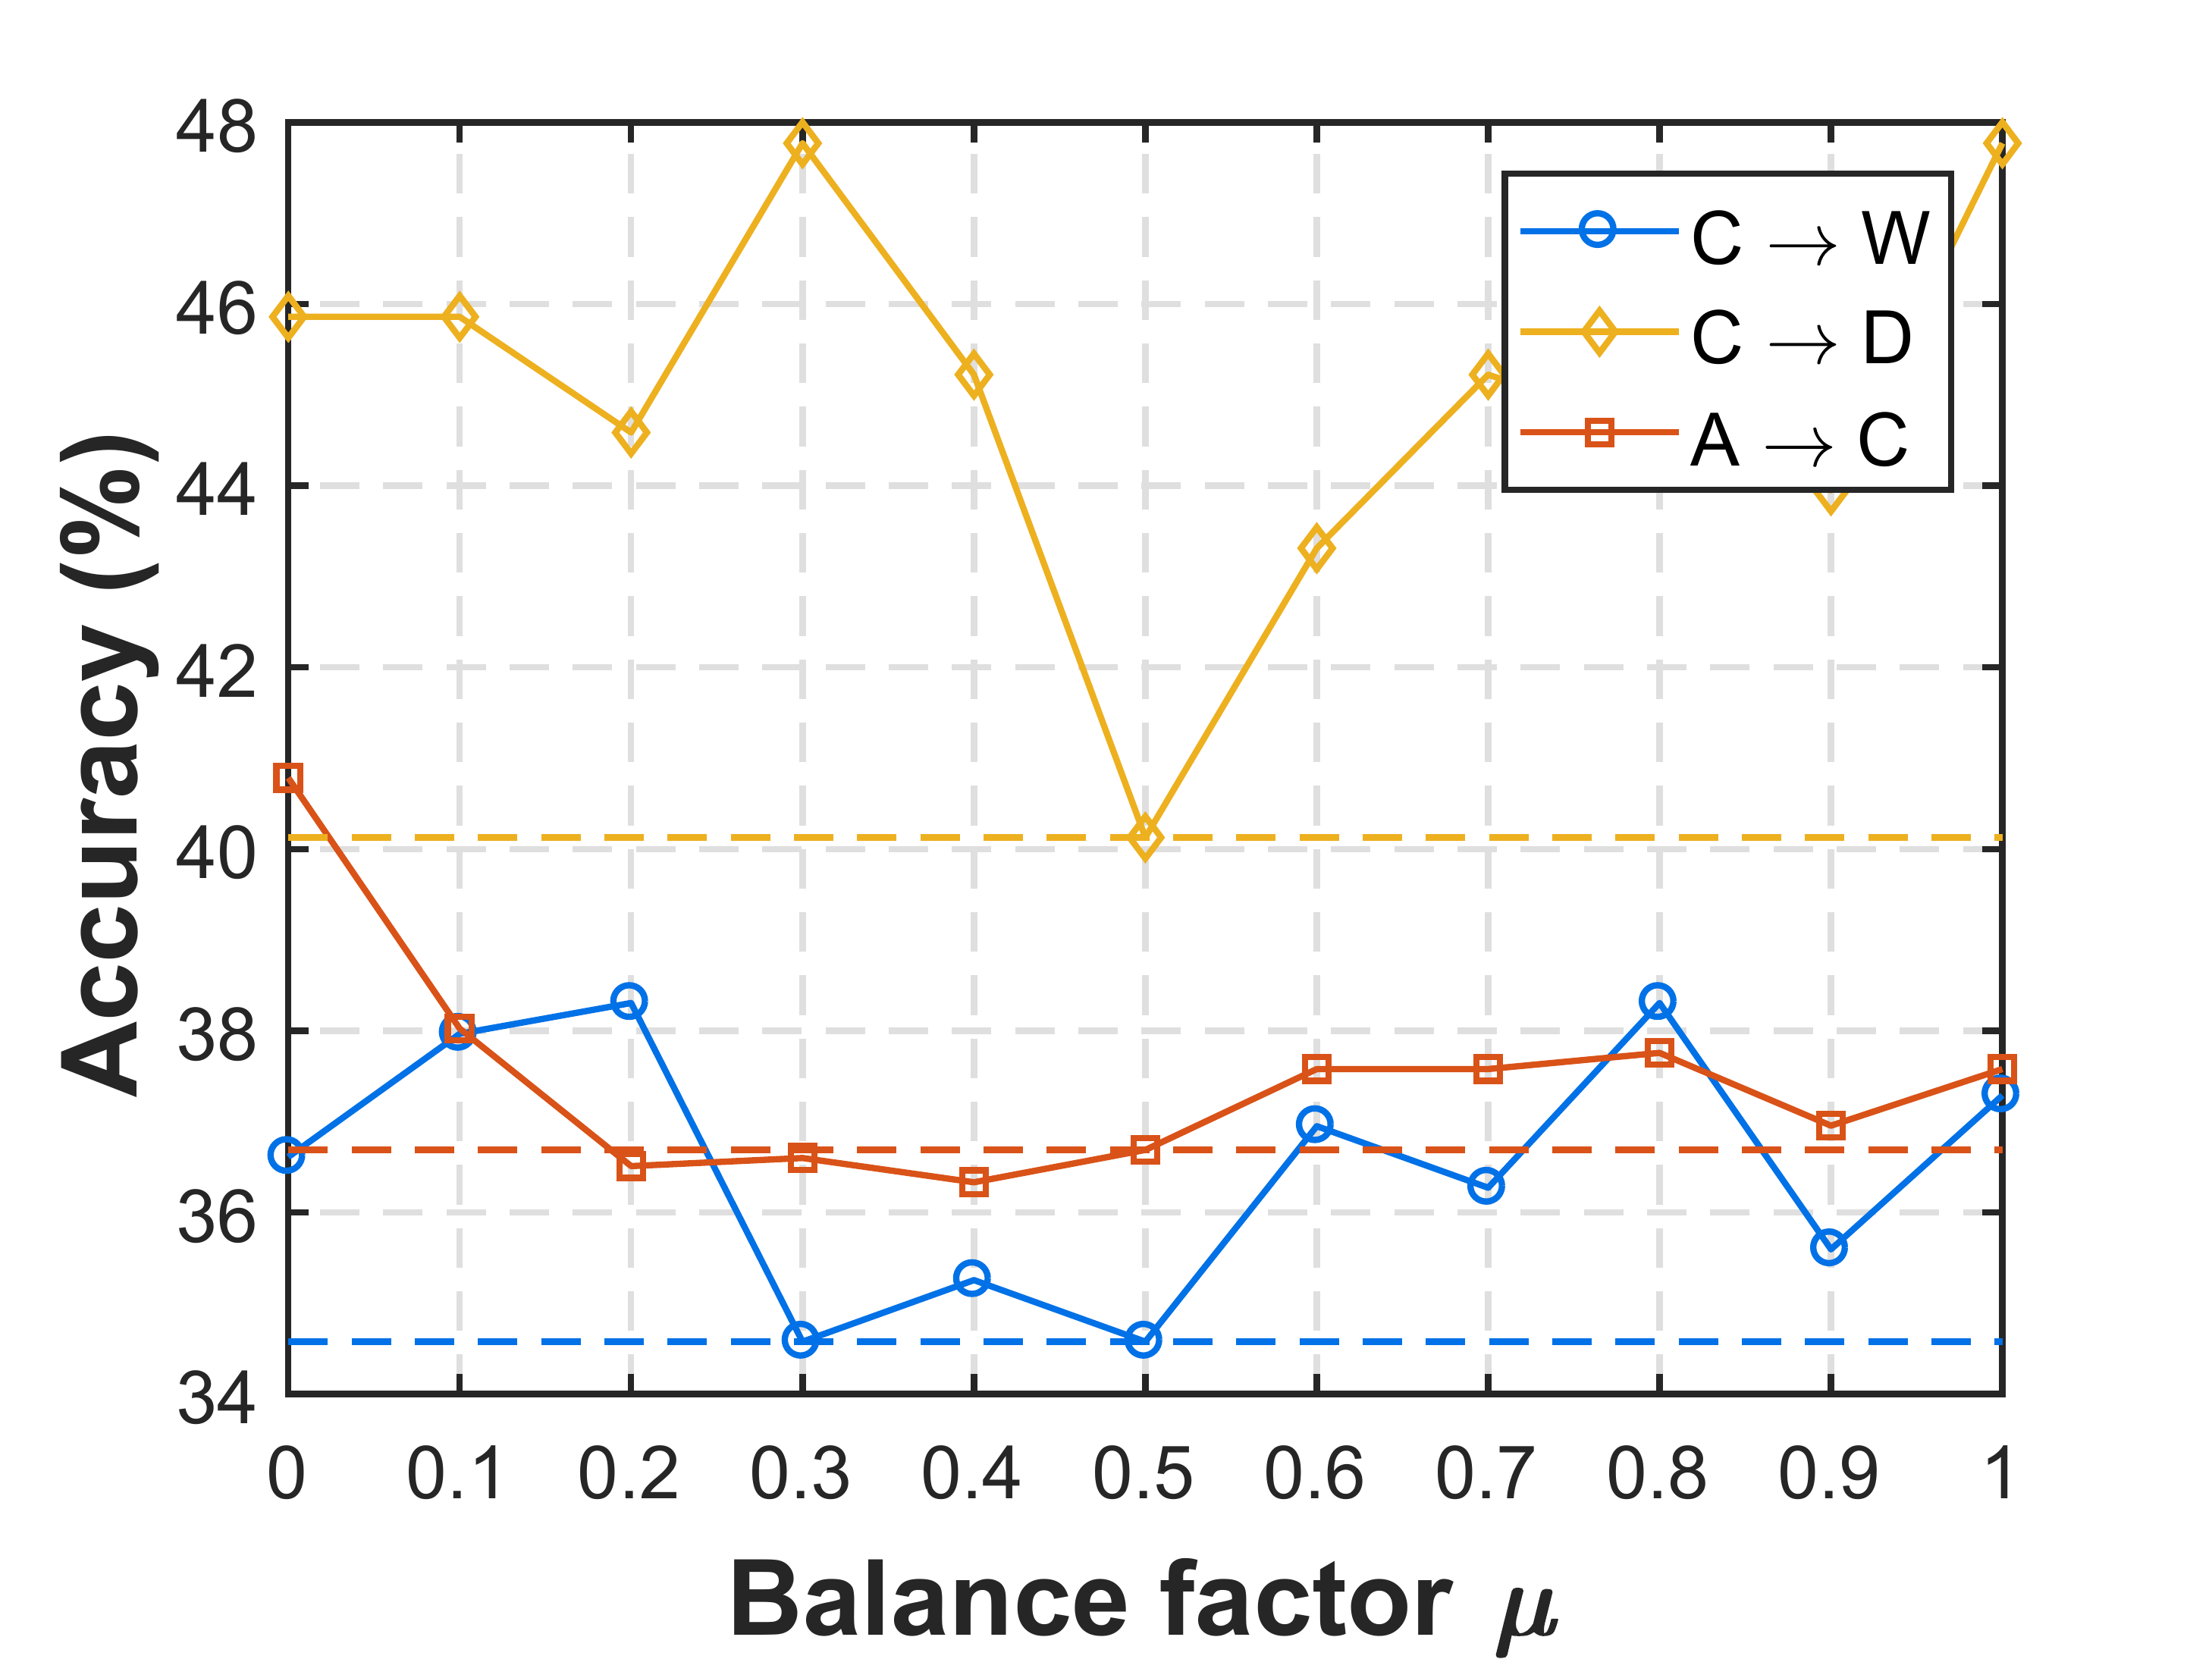
\includegraphics[scale=0.6]{./figures/fig-distribution-mu.pdf}
%	\caption{平衡因子$\mu$在分布自适应中的作用}
%	\label{fig-distribution-mu}
%\end{figure}

\begin{figure*}[h]
	\centering
	\subfigure[不同方法的MMD距离比较]{
		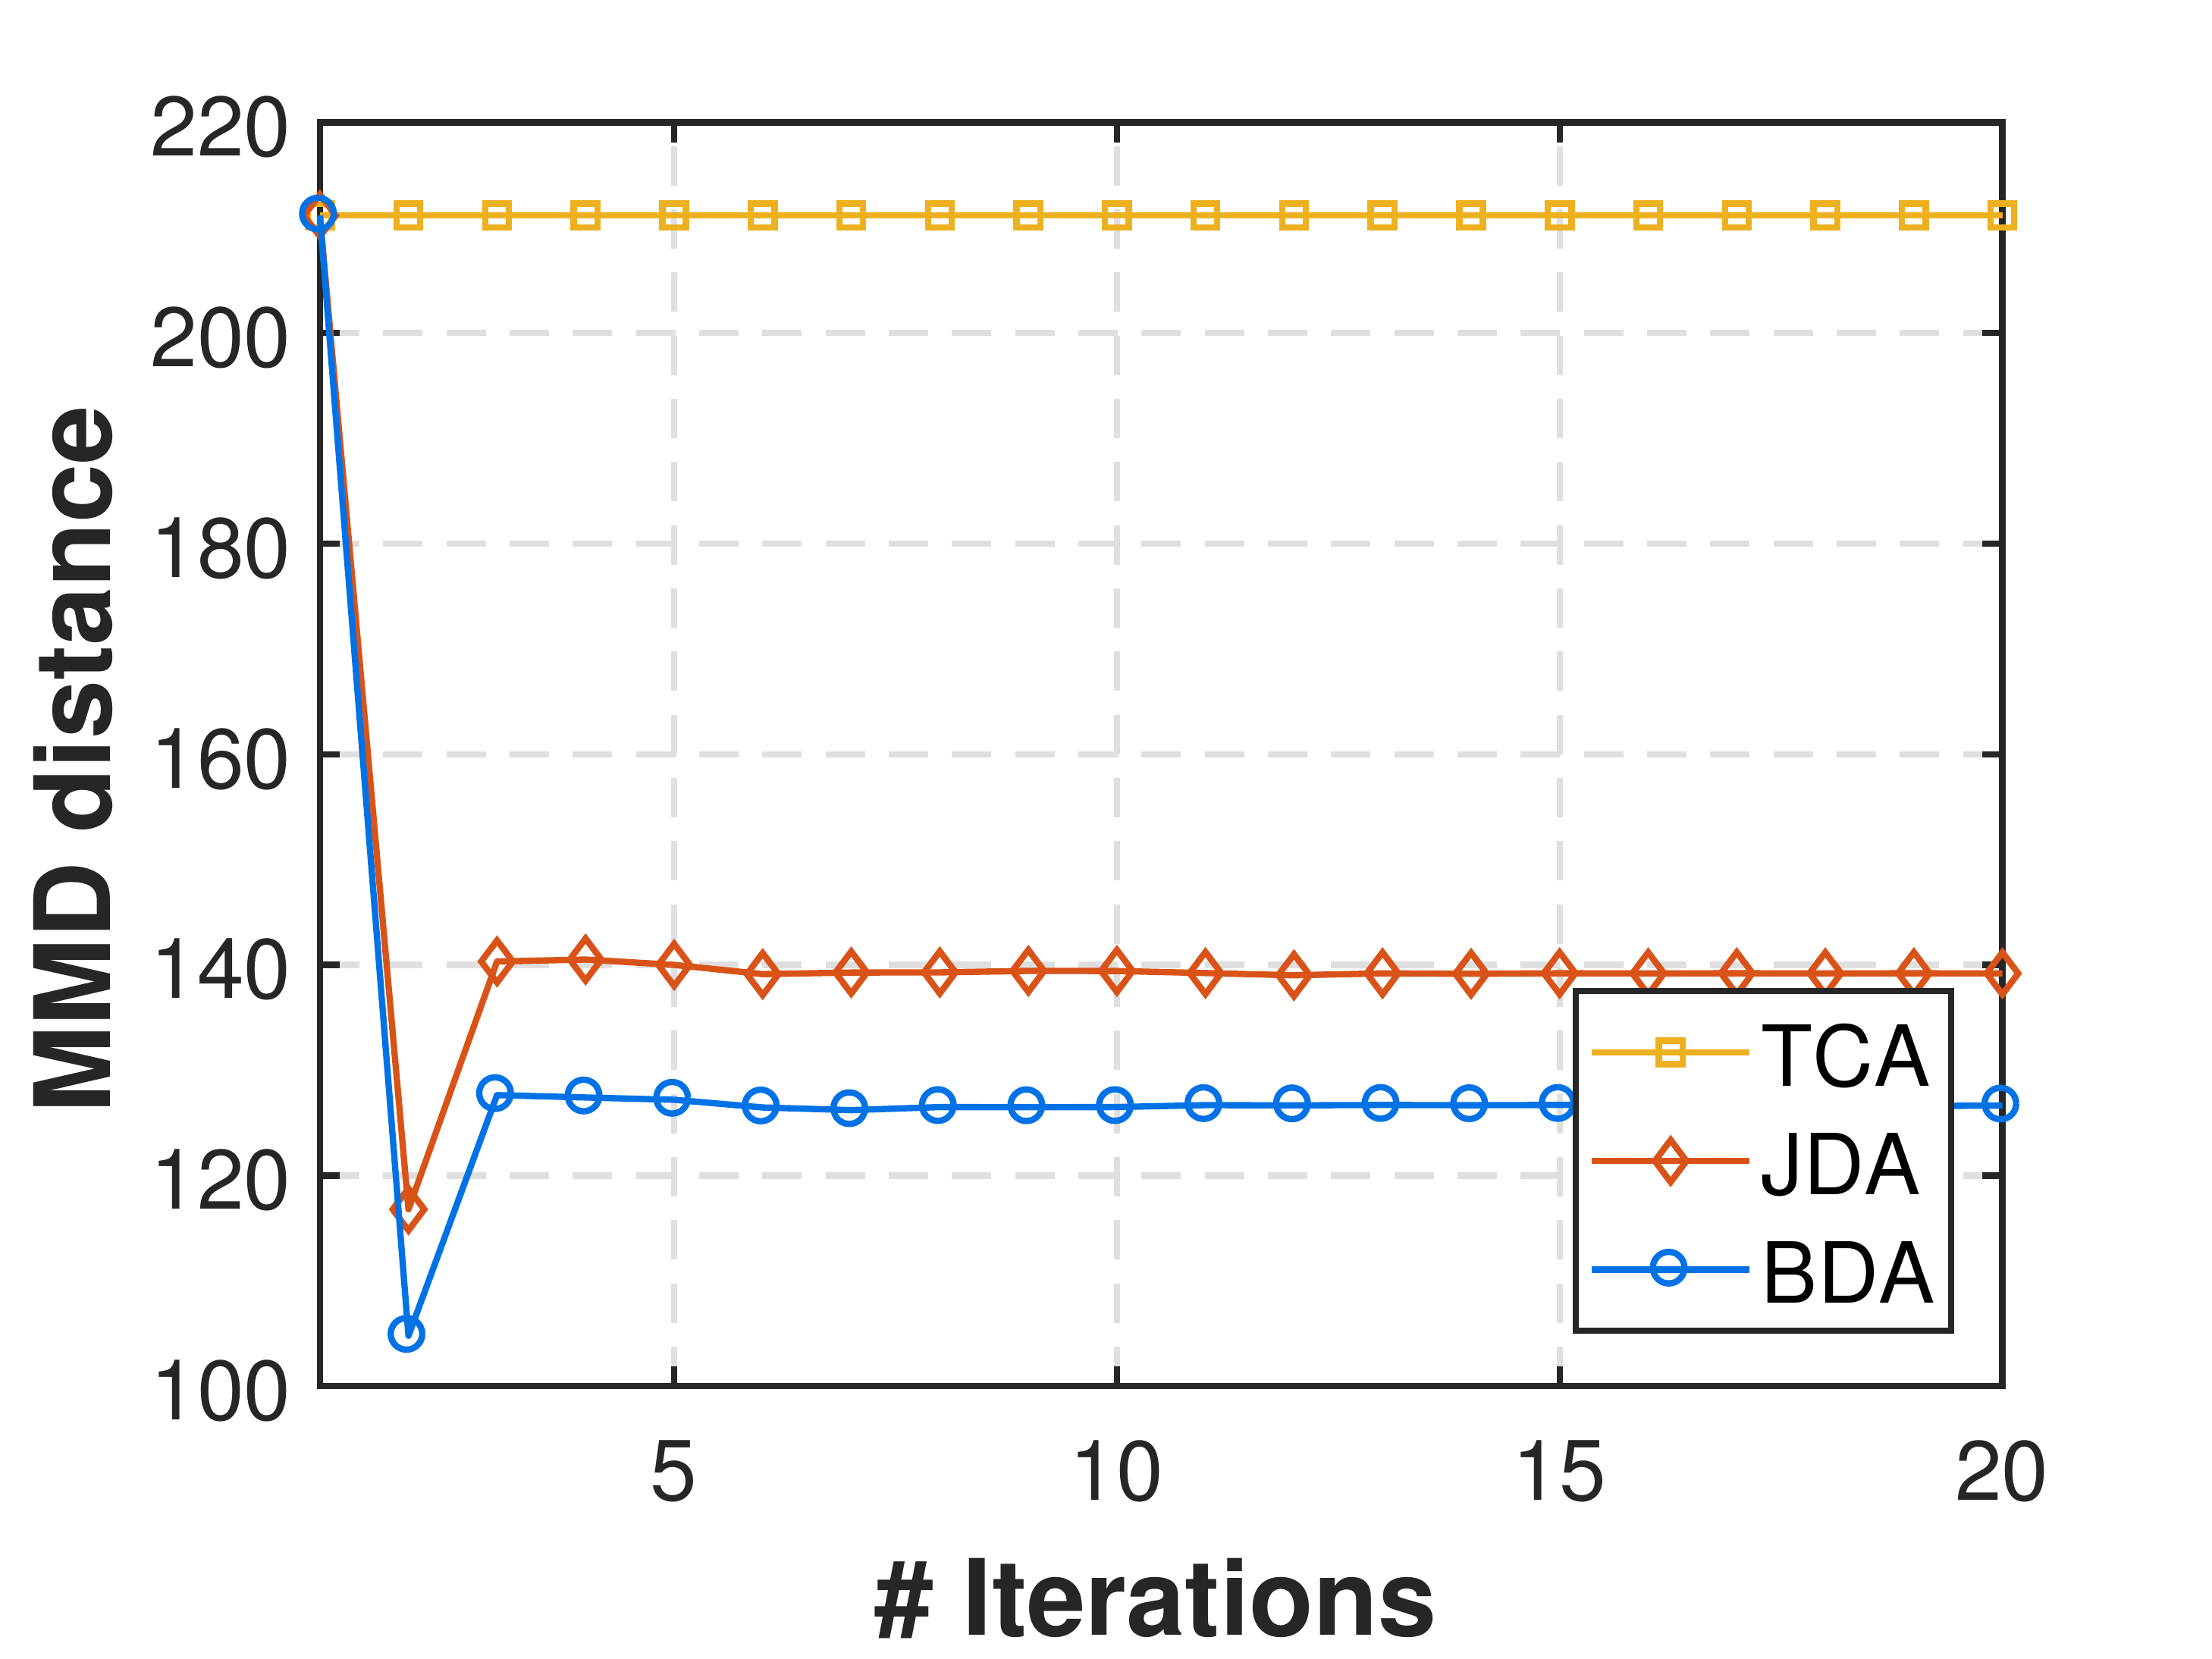
\includegraphics[scale=0.45]{./figures/fig-distribution-bdammd.pdf}
		\label{fig-distribution-mmd}}

	\subfigure[BDA方法中平衡因子$\mu$的作用]{
		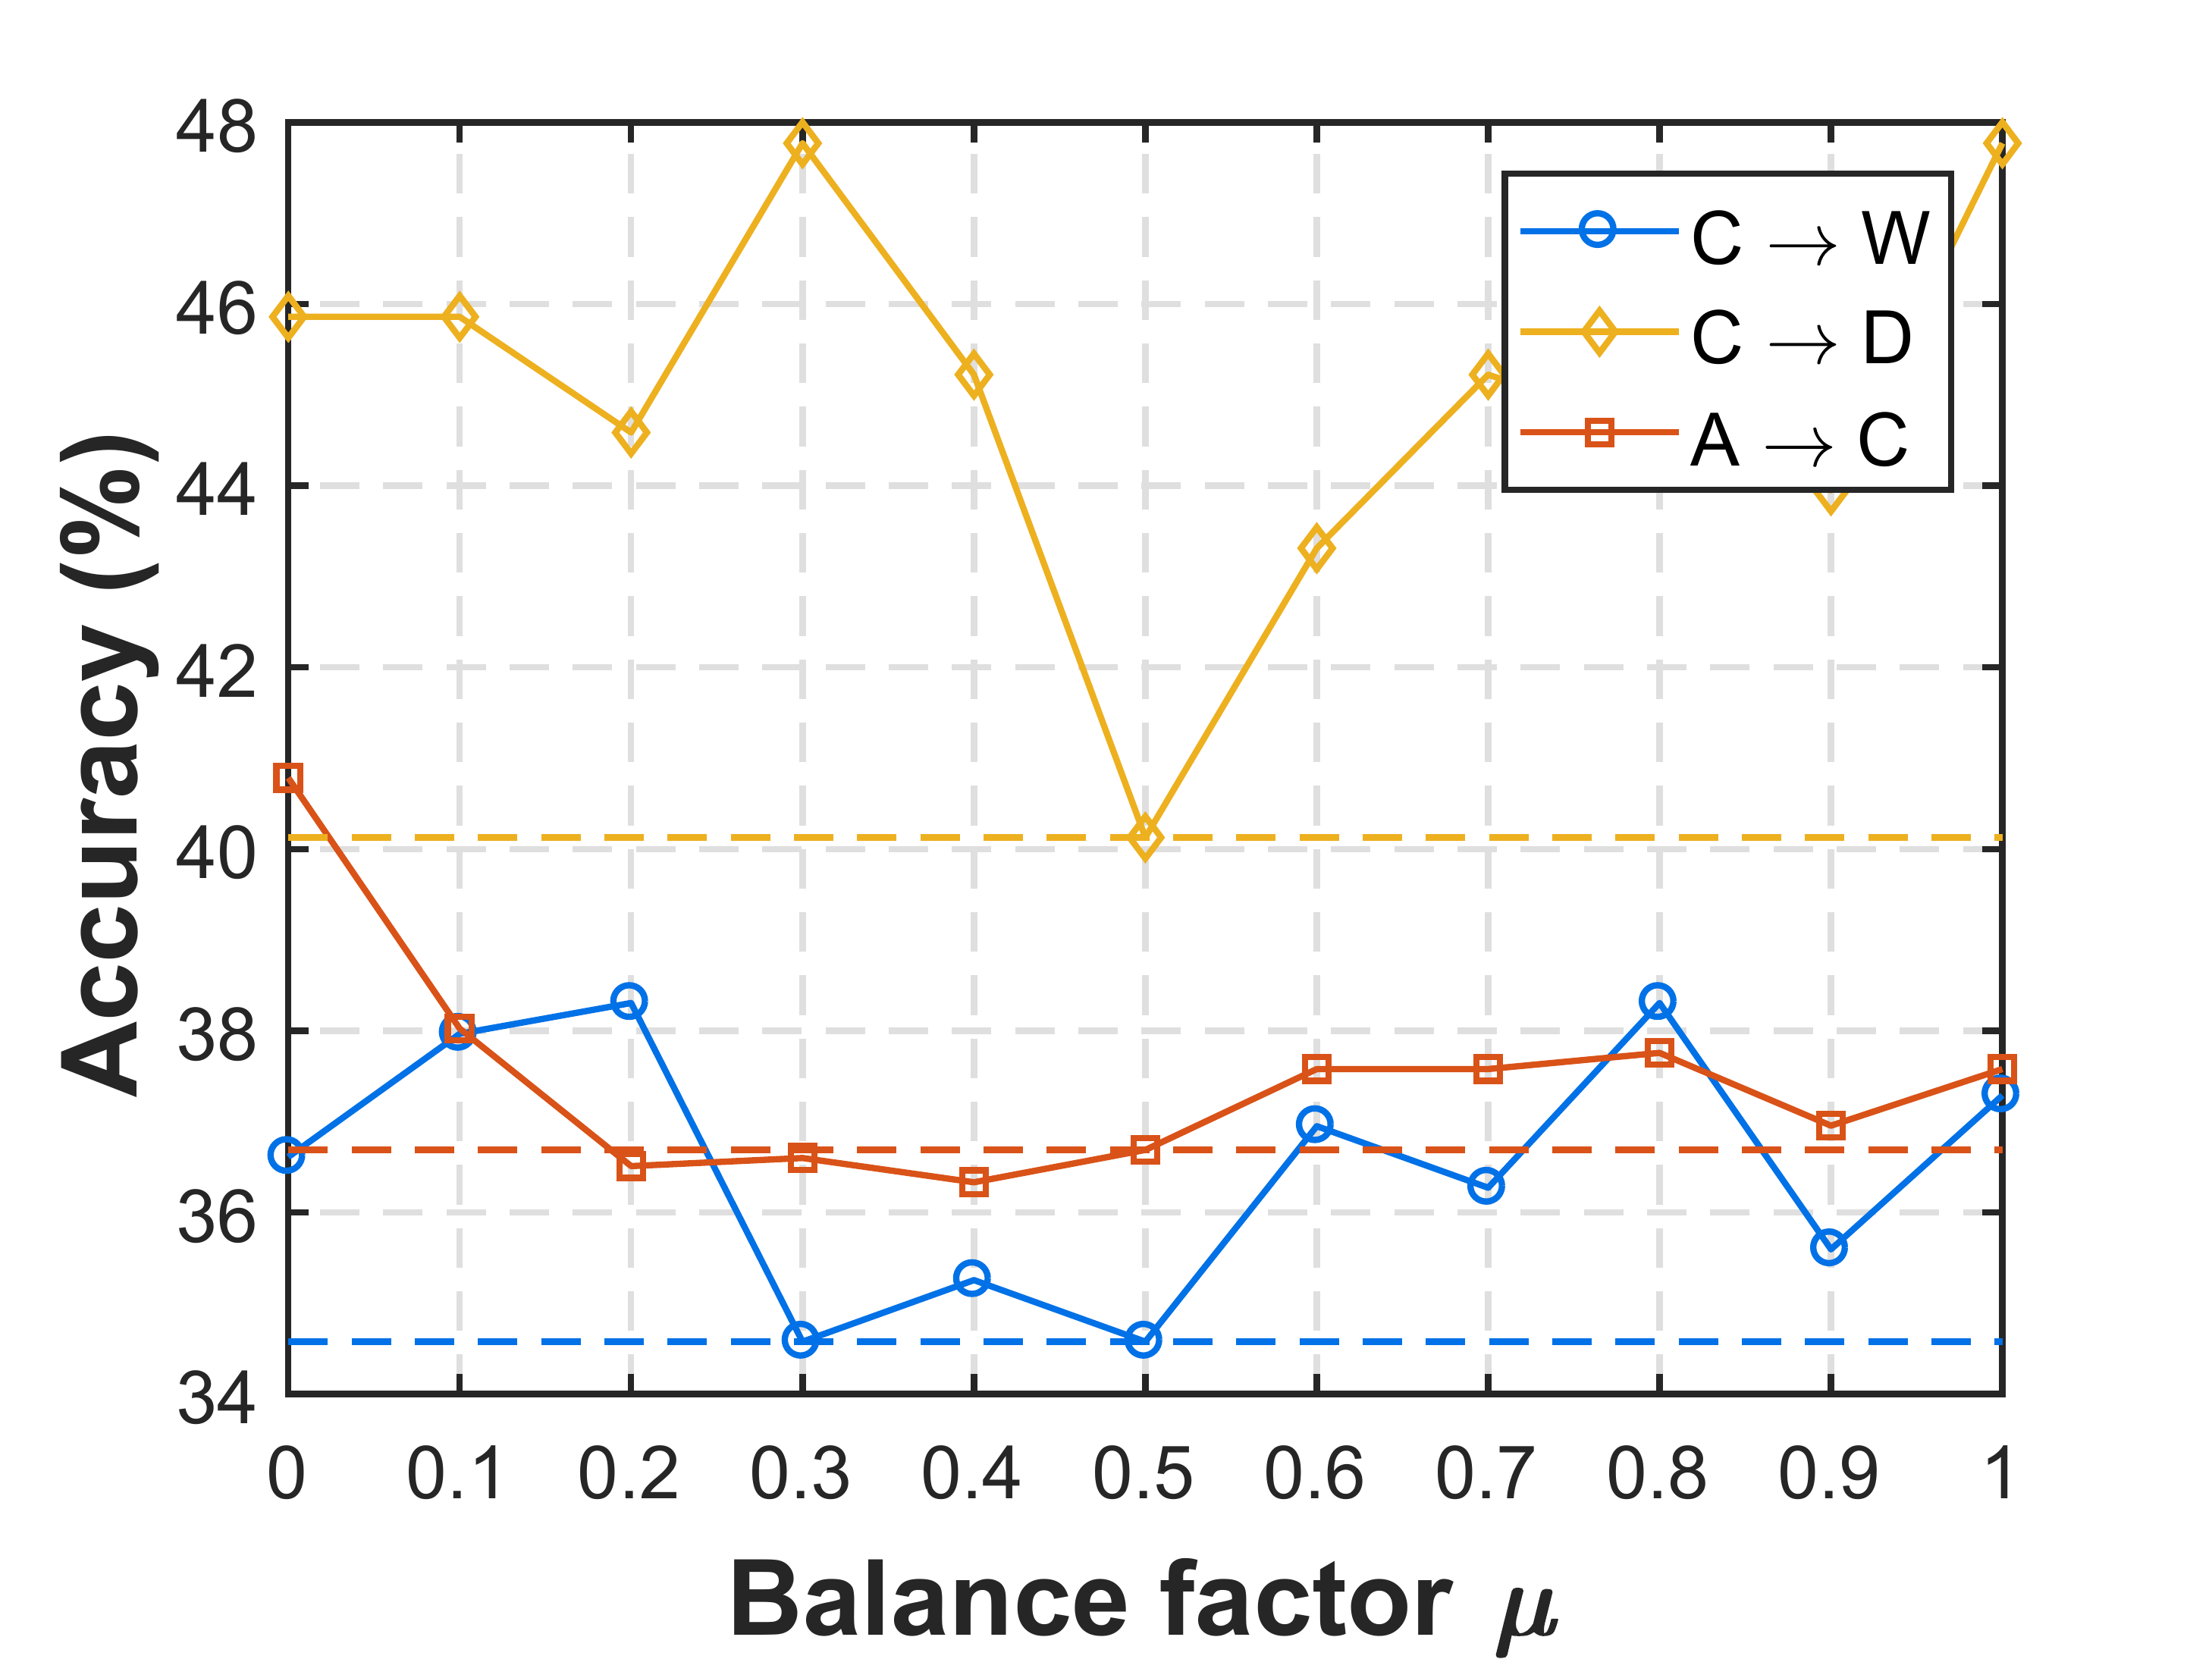
\includegraphics[scale=0.45]{./figures/fig-distribution-mu.pdf}
		\label{fig-distribution-mu}}
	\caption{BDA方法的效果}
	\label{fig-distribution-bda}
\end{figure*}

\textbf{动态分布自适应}

BDA方法是首次给出边缘分布和条件分布的定量估计。然而,其并未解决平衡因子$\mu$的精确计算问题。最近,作者扩展了BDA方法,提出了一个更具普适性的动态迁移框架DDA(Dynamic Distribution Adaptation)~\cite{wang2019transfer}来解决$\mu$值的精确估计问题。

注意到,可以简单地将$\mu$视为一个迁移过程中的参数,通过交叉验证 (cross-validation)来确定其最优的取值$\mu_{opt}$。然而,在本章的无监督迁移学习问题定义中,目标域完全没有标记,故此方式不可行。有另外两种非直接的方式可以对$\mu$值进行估计:随机猜测和最大最小平均法。随机猜测从神经网络随机调参中得到启发,指的是任意从$[0,1]$区间内选择一个$\mu$的值,然后进行动态迁移,其并不算是一种技术严密型的方案。如果重复此过程$t$次,记第$t$次的迁移学习结果为$r_t$,则随机猜测法最终的迁移结果为$r_{rand} = \frac{1}{t} \sum_{i=1}^{t} r_t$。最大最小平均法与随机猜测法相似,可以在$[0,1]$区间内从0开始取$\mu$的值,每次增加0.1,得到一个集合$[0,0.1,\cdots,0.9,1.0]$,然后,与随机猜测法相似,也可以得到其最终迁移结果$r_{maxmin}=\frac{1}{11} \sum_{i=1}^{11} r_i$。

然而,尽管上述两种估计方案有一定的可行性,它们均需要大量的重复计算,给普适计算设备带来了严峻的挑战。另外,上述结果并不具有可解释性,其正确性也无法得到保证。

作者提出的动态迁移方法是首次对$\mu$值进行精确的定量估计方法。该方法利用领域的整体和局部性质来定量计算$\mu$(计算出的值用$\hat{\mu}$来表示)。采用$\mathcal{A}-distance$~\cite{ben2007analysis}作为基本的度量方式。$\mathcal{A}-distance$被定义为建立一个二分类器进行两个不同领域的分类得出的误差。从形式化来看,定义$\epsilon(h)$作为线性分类器$h$区分两个领域$\Omega_s$和$\Omega_t$的误差。则,$\mathcal{A}-distance$可以被定义为:
\begin{equation}
d_A(\Omega_s,\Omega_t) = 2(1 - 2 \epsilon(h)).
\end{equation}

直接根据上式计算边缘分布的$\mathcal{A}-distance$,将其用$d_M$来表示。对于条件分布之间的$\mathcal{A}-distance$,用$d_c$来表示对应于类别$c$的条件分布距离。它可以由式$d_c = d_A(\Omega^{(c)}_s,\Omega^{(c)}_t)$进行计算,其中$\Omega^{(c)}_s$和$\Omega^{(c)}_t$分别表示来自源域和目标域的第$c$个类的样本。最终,$\mu$可以由下式进行计算:
\begin{equation}
\label{eq-meda-mu}
\hat{\mu} = 1 - \frac{d_M}{d_M + \sum_{c=1}^{C} d_c}.
\end{equation}

由于特征的动态和渐近变化性,此估计需要在每一轮迭代中给出。值得注意的是,这是\textbf{首次}给出边缘分布和条件分布的定量估计,对于迁移学习研究具有很大的意义。

具体而言,作者将机器学习问题规约成一个统计机器学习问题,可以用统计机器学习中的结构风险最小化的原则(Structural Risk Minimization, SRM)~\cite{belkin2006manifold,vapnik1998statistical}进行表示学习。在SRM中,分类器$f$可以被表示为:
\begin{equation}
\label{eq-meda-srm}
f = \mathop{\arg\min}_{f \in \mathcal{H}_{K}, (\mathbf{x},y) \sim \Omega_l} J(f(\mathbf{x}),y) + R(f),
\end{equation}
其中第一项表示$f$在有标记数据上的损失,第二项为正则项,$\mathcal{H}_{K}$表示核函数$K(\cdot,\cdot)$构造的希尔伯特空间 (Hilbert space)。符号$\Omega_l$表示有标记的数据领域。在本章的问题中,$\Omega_l = \Omega_s$,即只有源域数据有标记。特别地,由于在迁移学习问题中,源域和目标域数据有着不同的数据分布,为了表示此分布距离,可以进一步将正则项表示成如下的形式:
\begin{equation}
R(f) = \lambda \overline{D_f}(\Omega_s,\Omega_t) + R_f(\Omega_s,\Omega_t),
\end{equation}
其中$\overline{D_f}(\cdot, \cdot)$表示$\Omega_s$和$\Omega_t$的分布距离,$\lambda$为平衡系数,$R_f(\cdot, \cdot)$则为其他形式的正则项。根据公式~(\ref{eq-meda-srm})中的结构风险最小化公式,如果用$g(\cdot)$来表示特征学习过程,则$f$可以被表示为:
\begin{equation}
\label{equ-f-orig}
f = \mathop{\arg\min}_{f \in \sum_{i=1}^{n} \mathcal{H}_{K}} J(f(g(\mathbf{x}_i)),y_i) + \eta ||f||^2_K + \lambda \overline{D_f}(\Omega_s,\Omega_t) + \rho R_f(\Omega_s,\Omega_t),
\end{equation}
其中$||f||^2_K$是$f$的平方标准形式。$\overline{D_f}(\cdot,\cdot)$这一项表示本章提出的动态迁移学习。引入拉普拉斯约束作为$f$的额外正则项~\cite{belkin2006manifold}。$\eta,\lambda$,和$\rho$是对应的正则项系数。

上式则为通用的一个迁移学习框架,可以适用于任何问题。为了对此框架进行学习,作者分别提出了基于流形学习的动态迁移方法MEDA (Manifold Embedded Distribution Alignment)~\cite{wang2018visual}和基于深度学习的动态迁移方法DDAN (Deep Dynamic Adaptation Network)~\cite{wang2019transfer}来进行学习。这两种方法分别如图~\ref{fig-distribution-meda}和~\ref{fig-distribution-ddan}所示。

%\begin{figure}[t!]
%	\centering
%	\begin{subfigure}[1]{0.48\textwidth}
%		\includegraphics[width=\textwidth]{./figures/fig-meda-main.pdf}
%		\caption{流形空间动态迁移MEDA}
%		\label{fig-meda-manifold}
%	\end{subfigure}
%	
%	\hspace{.2in}
%	
%	\begin{subfigure}[1]{0.48\textwidth}
%		\includegraphics[width=\textwidth]{./figures/fig-meda-deep.pdf}
%		\caption{深度网络动态迁移DDAN}
%		\label{fig-meda-deep}
%	\end{subfigure}
%	\caption{基于流形学习和深度学习的动态迁移方法MDDA和DDAN}
%	\label{fig-meda-main}
%\end{figure}

\begin{figure*}[h]
	\centering
	\subfigure[流形空间动态迁移MEDA]{
		\includegraphics[scale=0.45]{./figures/fig-meda-main.pdf}
		\label{fig-distribution-meda}}
	
	\subfigure[深度网络动态迁移DDAN]{
		\includegraphics[scale=0.45]{./figures/fig-meda-deep.pdf}
		\label{fig-distribution-ddan}}
	\caption{动态分布自适应}
	\label{fig-distribution-dda}
\end{figure*}

最近,作者在~\cite{yu2019transfer}中将DDA的概念进一步扩展到了对抗网络中,证明了对抗网络中同样存在边缘分布和条件分布不匹配的问题。作者提出一个动态对抗适配网络DAAN (Dynamic Adversarial Adaptation Networks)来解决对抗网络中的动态分布适配问题,取得了当前的最好效果。图~\ref{fig-daan}展示了DAAN的架构。

\begin{figure}[htbp]
	\centering
	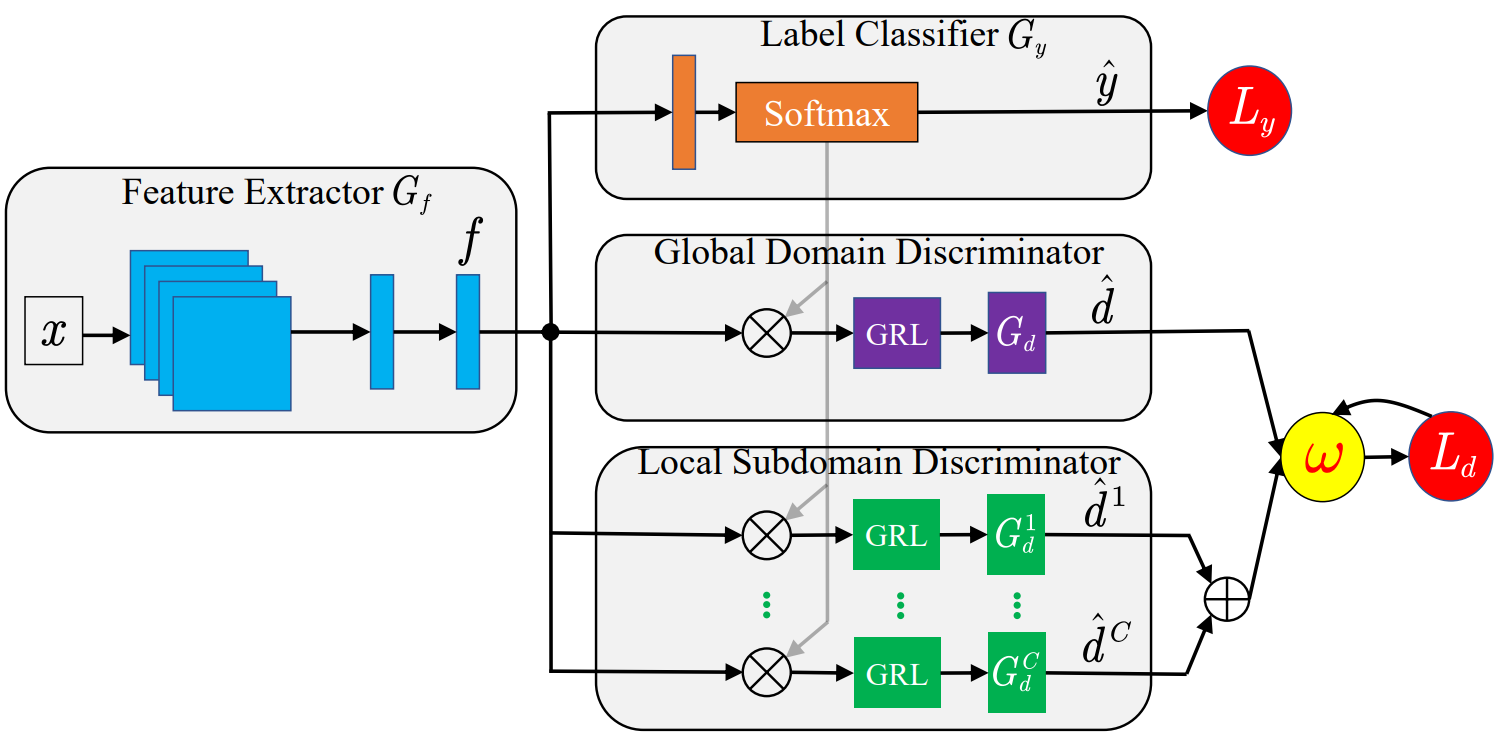
\includegraphics[scale=.35]{./figures/fig-distribution-daan.png}
	\caption{动态对抗适配网络DAAN结构示意图}
	\label{fig-daan}
\end{figure}

\subsection{小结}

综合上述三种概率分布自适应方法,我们可以得出如下的结论:

\begin{enumerate}
	\item 精度比较:DDA > JDA > TCA > 条件分布自适应。
	\item 将不同的概率分布自适应方法用于神经网络,是一个发展趋势。将概率分布适配加入深度网络中,往往会取得比非深度方法更好的结果。
\end{enumerate}


\input{chaps/ch07_featureselect}
\input{chaps/ch08_subspacelearn}
\newpage
\section{深度迁移学习}

随着深度学习方法的大行其道,越来越多的研究人员使用深度神经网络进行迁移学习。对比传统的非深度迁移学习方法,深度迁移学习直接提升了在不同任务上的学习效果。并且,由于深度学习直接对原始数据进行学习,所以其对比非深度方法还有两个优势:\textit{自动化地提取更具表现力的特征},以及\textit{满足了实际应用中的端到端(End-to-End)需求}。

近年来,以生成对抗网络(Generative Adversarial Nets, GAN)~\cite{goodfellow2014generative}为代表的对抗学习也吸引了很多研究者的目光。基于GAN的各种变体网络不断涌现。对抗学习网络对比传统的深度神经网络,极大地提升了学习效果。因此,基于对抗网络的迁移学习,也是一个热门的研究点。

图~\ref{fig-deep}展示了近几年的一些代表性方法在相同数据集上的表现。从图中的结果我们可以看出,深度迁移学习方法(BA、DDC、DAN)对比传统迁移学习方法(TCA、GFK等),在精度上具有无可匹敌的优势。

\begin{figure}[htbp]
	\centering
	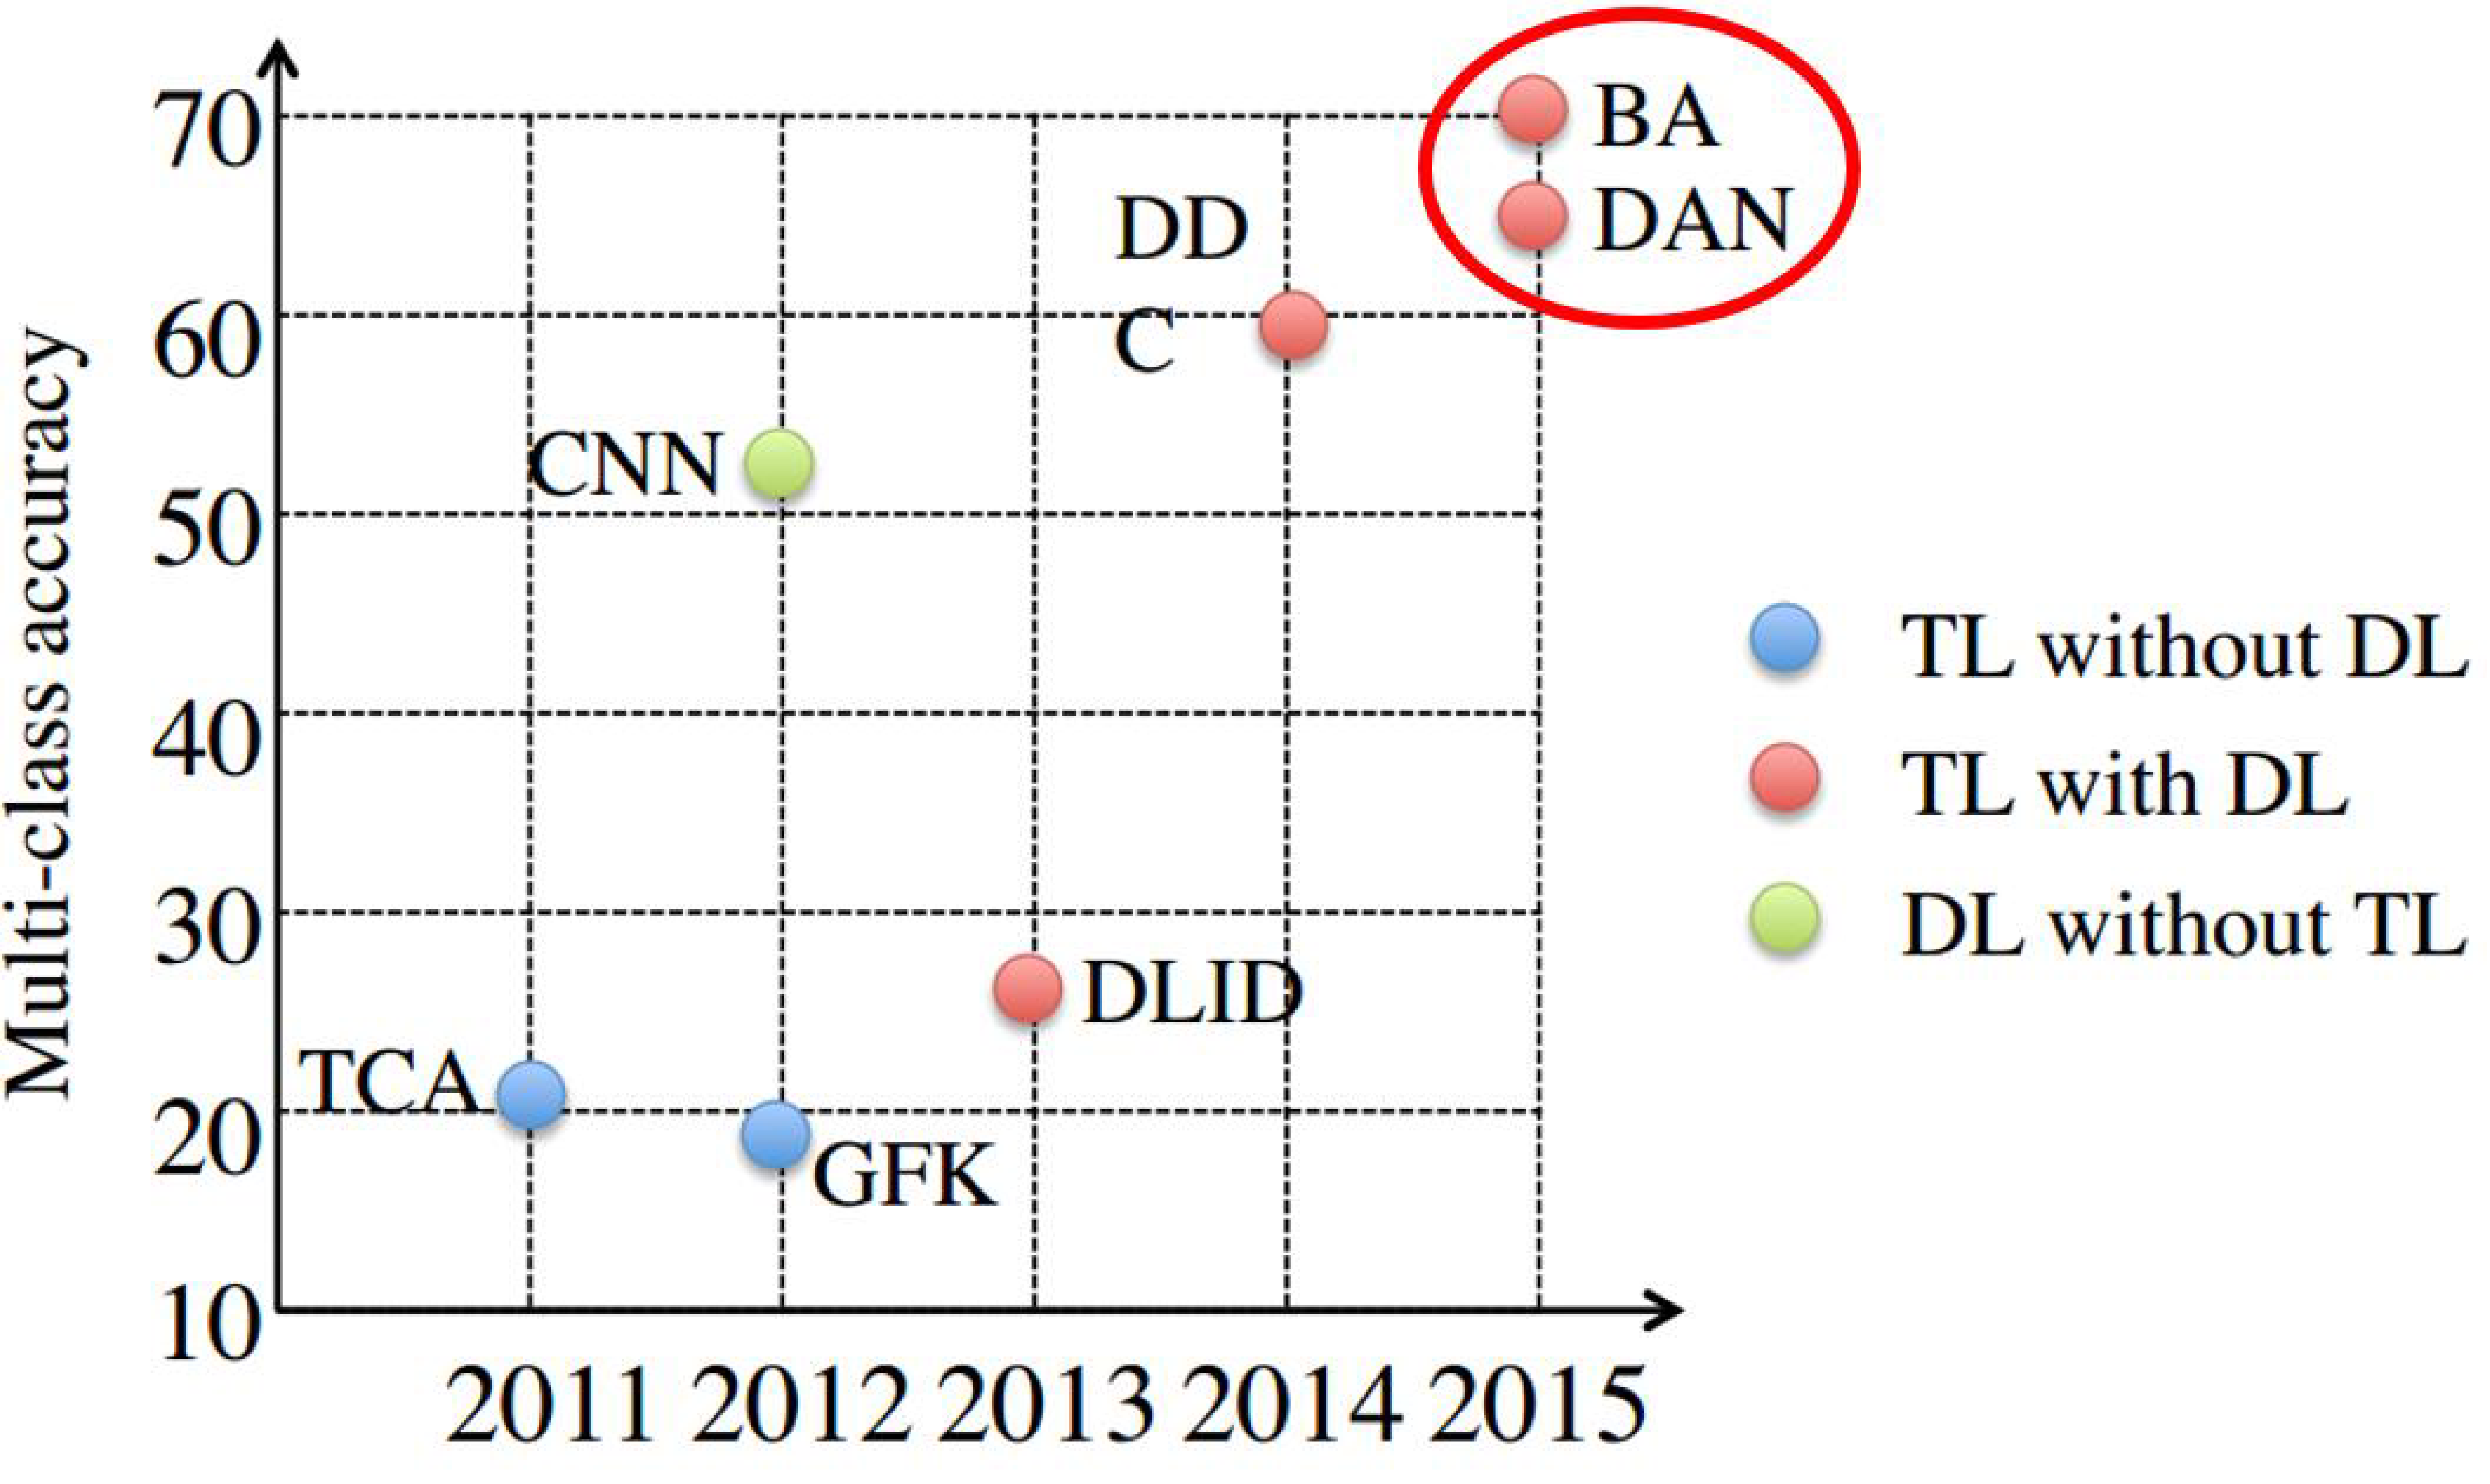
\includegraphics[scale=0.42]{./figures/fig-deep-compare.pdf}
	\caption{深度与非深度迁移学习方法的结果对比}
	\label{fig-deep}
\end{figure}

本部分重点介绍深度迁移学习的基本思路。首先我们回答一个最基本的问题:\textit{为什么深度网络是可迁移的}?然后,我们介绍最简单的深度网络迁移形式:finetune。接着分别介绍使用深度网络和深度对抗网络进行迁移学习的基本思路和核心方法。值得注意的是,由于深度迁移学习方面的研究工作层出不穷,我们不可能覆盖到所有最新的方法。但是基本上,这些方法的原理都大同小异。因此,我们的介绍是具有普适性的。

\subsection{深度网络的可迁移性}
随着AlexNet~\cite{krizhevsky2012imagenet}在2012年的ImageNet大赛上获得冠军,深度学习开始在机器学习的研究和应用领域大放异彩。尽管取得了很好的结果,但是神经网络本身就像一个黑箱子,看得见,摸不着,解释性不好。由于神经网络具有良好的层次结构,很自然地就有人开始关注,能否通过这些层次结构来很好地解释网络?于是,有了我们熟知的例子:假设一个网络要识别一只猫,那么一开始它只能检测到一些边边角角的东西,和猫根本没有关系;然后可能会检测到一些线条和圆形;慢慢地,可以检测到有猫的区域;接着是猫腿、猫脸等等。图~\ref{fig-whydeep}是一个简单的示例。

\begin{figure}[htbp]
	\centering
	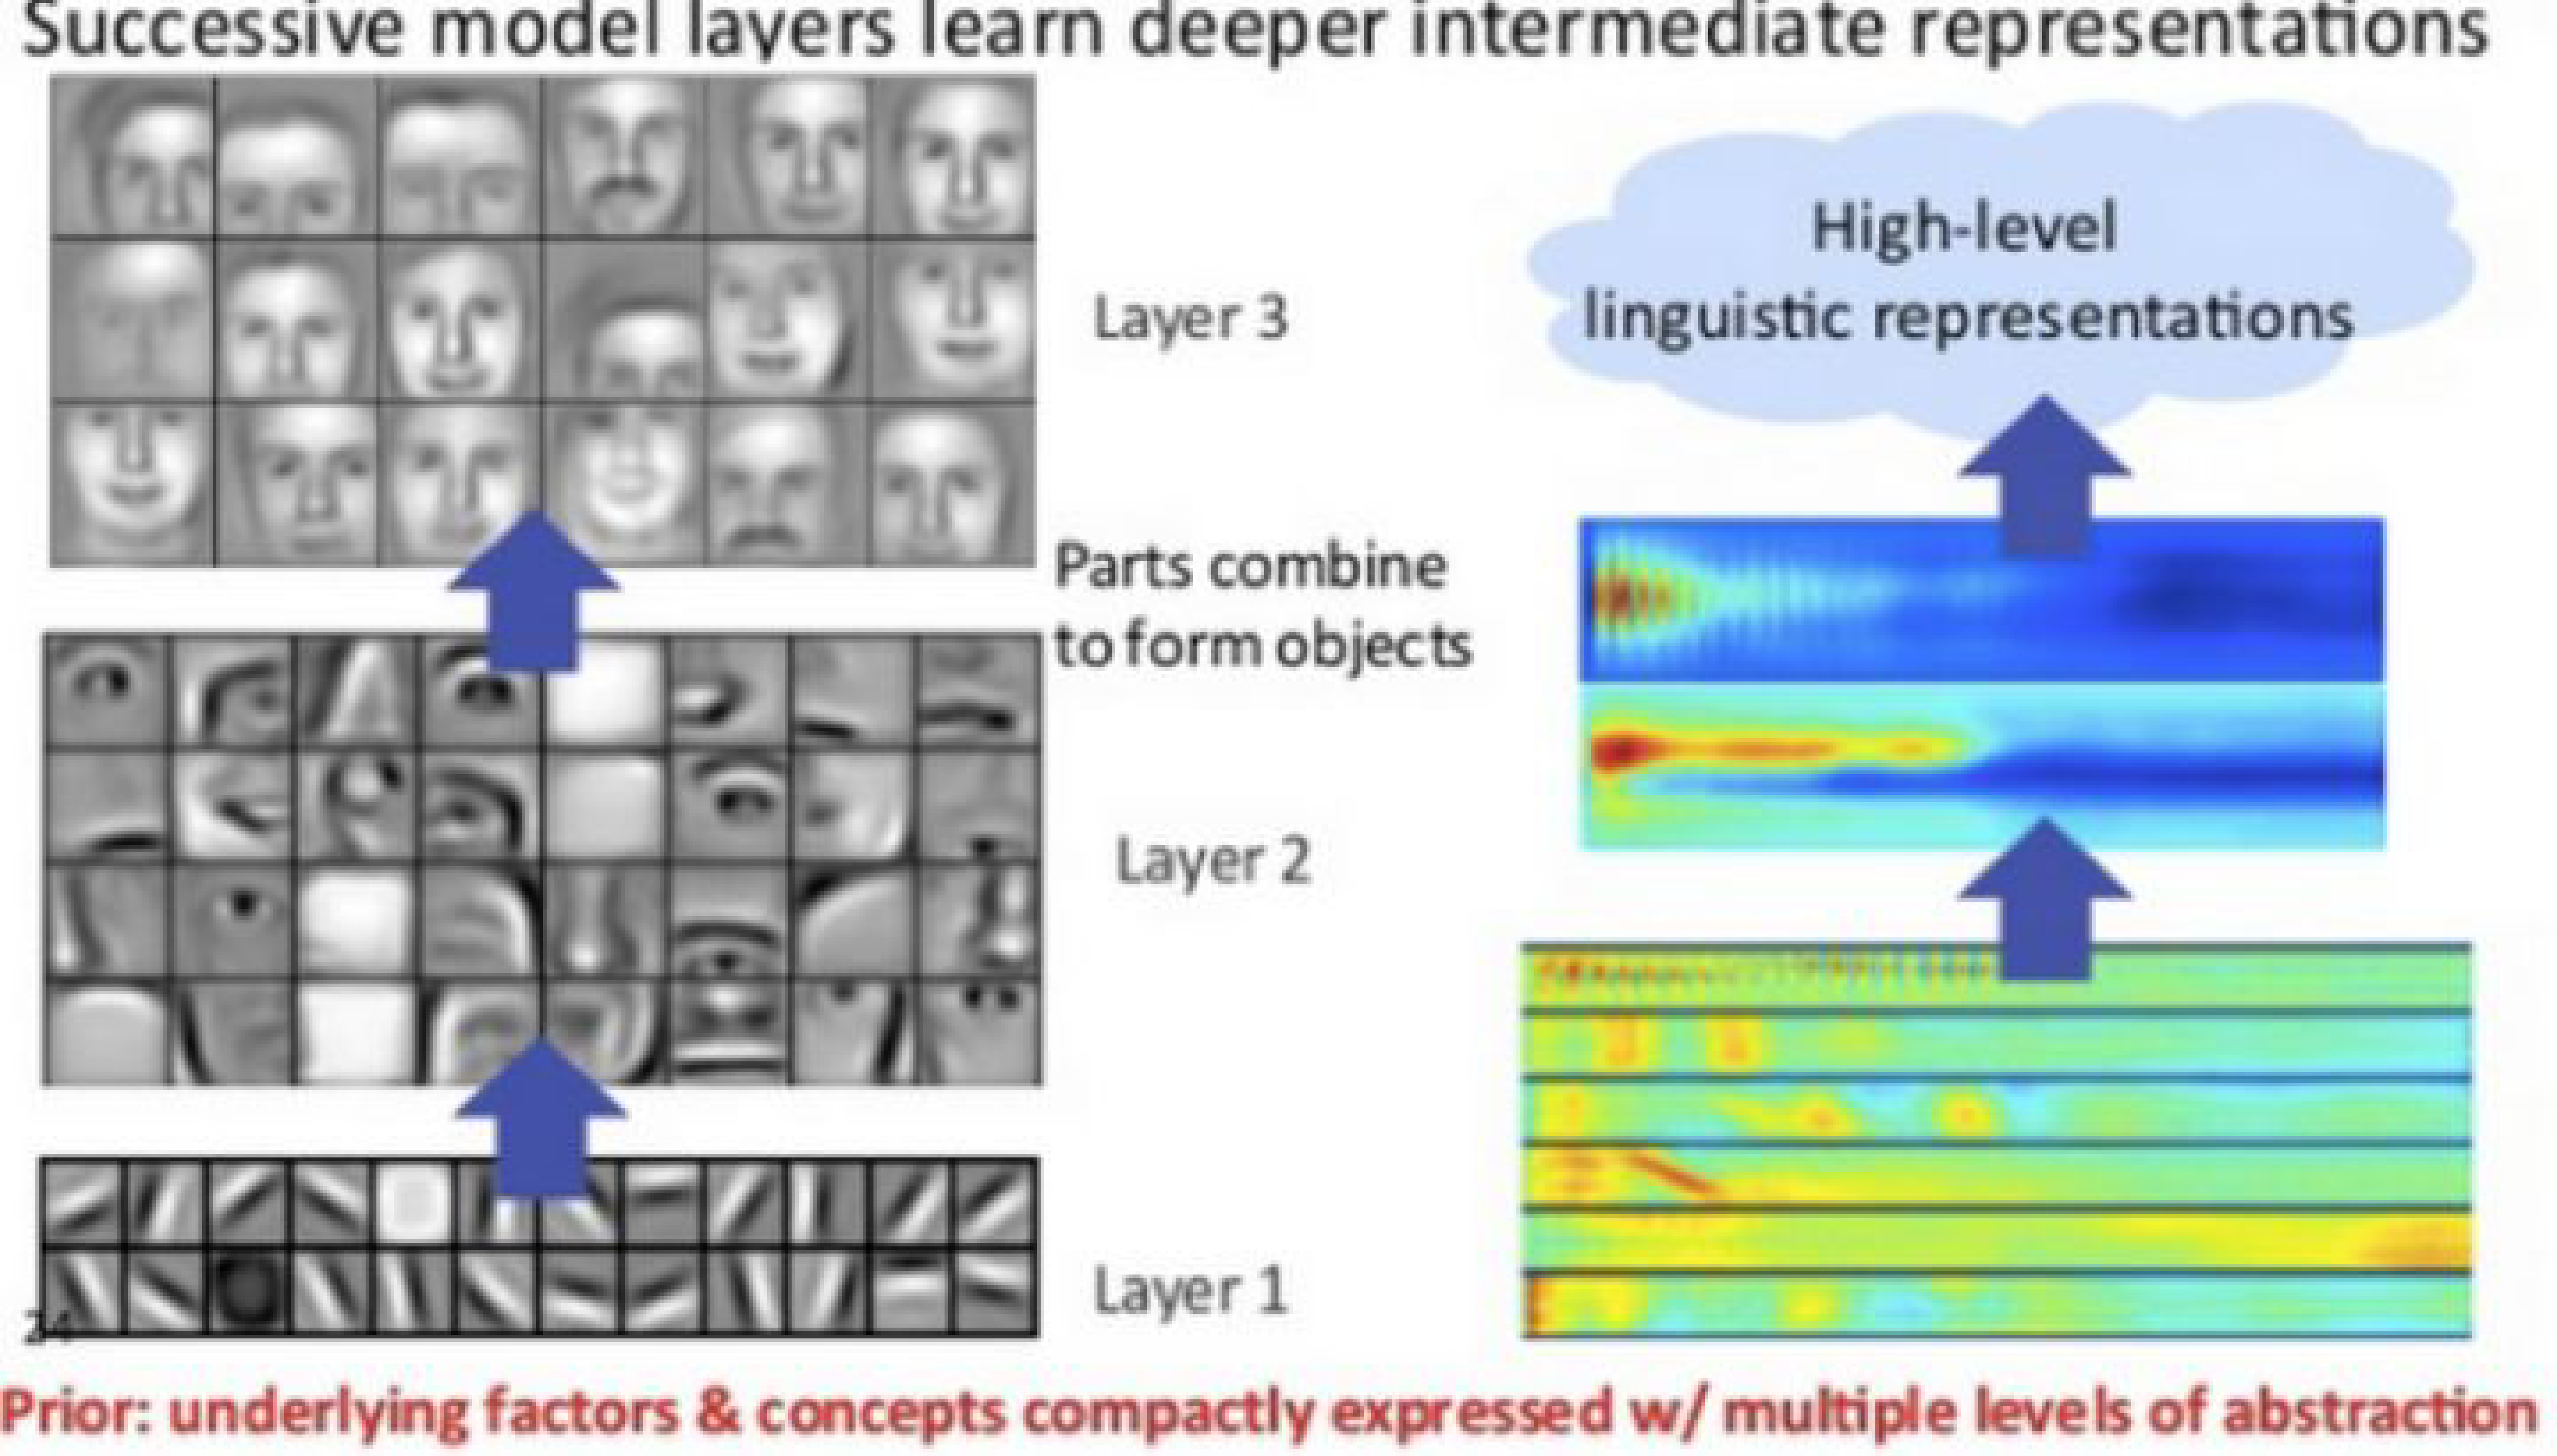
\includegraphics[scale=0.5]{./figures/fig-whydeep.pdf}
	\caption{深度神经网络进行特征提取到分类的简单示例}
	\label{fig-whydeep}
\end{figure}

这表达了一个什么事实呢?概括来说就是:前面几层都学习到的是通用的特征(general feature);随着网络层次的加深,后面的网络更偏重于学习任务特定的特征(specific feature)。这非常好理解,我们也都很好接受。那么问题来了:如何得知哪些层能够学习到general feature,哪些层能够学习到specific feature。更进一步:\textit{如果应用于迁移学习,如何决定该迁移哪些层、固定哪些层?}

这个问题对于理解神经网络以及深度迁移学习都有着非常重要的意义。

来自康奈尔大学的Jason Yosinski等人~\cite{yosinski2014transferable}率先进行了深度神经网络可迁移性的研究,将成果发表在2014年机器学习领域顶级会议NIPS上并做了口头汇报。该论文是一篇实验性质的文章(通篇没有一个公式)。其目的就是要探究上面我们提到的几个关键性问题。因此,文章的全部贡献都来自于实验及其结果。(别说为啥做实验也能发文章:都是高考,我只上了个普通一本,我高中同学就上了清华)

在ImageNet的1000类上,作者把1000类分成两份(A和B),每份500个类别。然后,分别对A和B基于Caffe训练了一个AlexNet网络。一个AlexNet网络一共有8层,除去第8层是类别相关的网络无法迁移以外,作者在1到7这7层上逐层进行finetune实验,探索网络的可迁移性。

为了更好地说明finetune的结果,作者提出了有趣的概念:AnB和BnB。

迁移A网络的前$n$层到B(AnB) vs 固定B网络的前$n$层(BnB)

简单说一下什么叫AnB:(所有实验都是针对数据B来说的)将A网络的前$n$层拿来并将它frozen,剩下的$8-n$层随机初始化,然后对B进行分类。

相应地,有BnB:把训练好的B网络的前$n$层拿来并将它frozen,剩下的$8-n$层随机初始化,然后对B进行分类。

\textbf{实验结果}

实验结果如下图(图~\ref{fig-8-2})所示:

\begin{figure}[htbp]
	\centering
	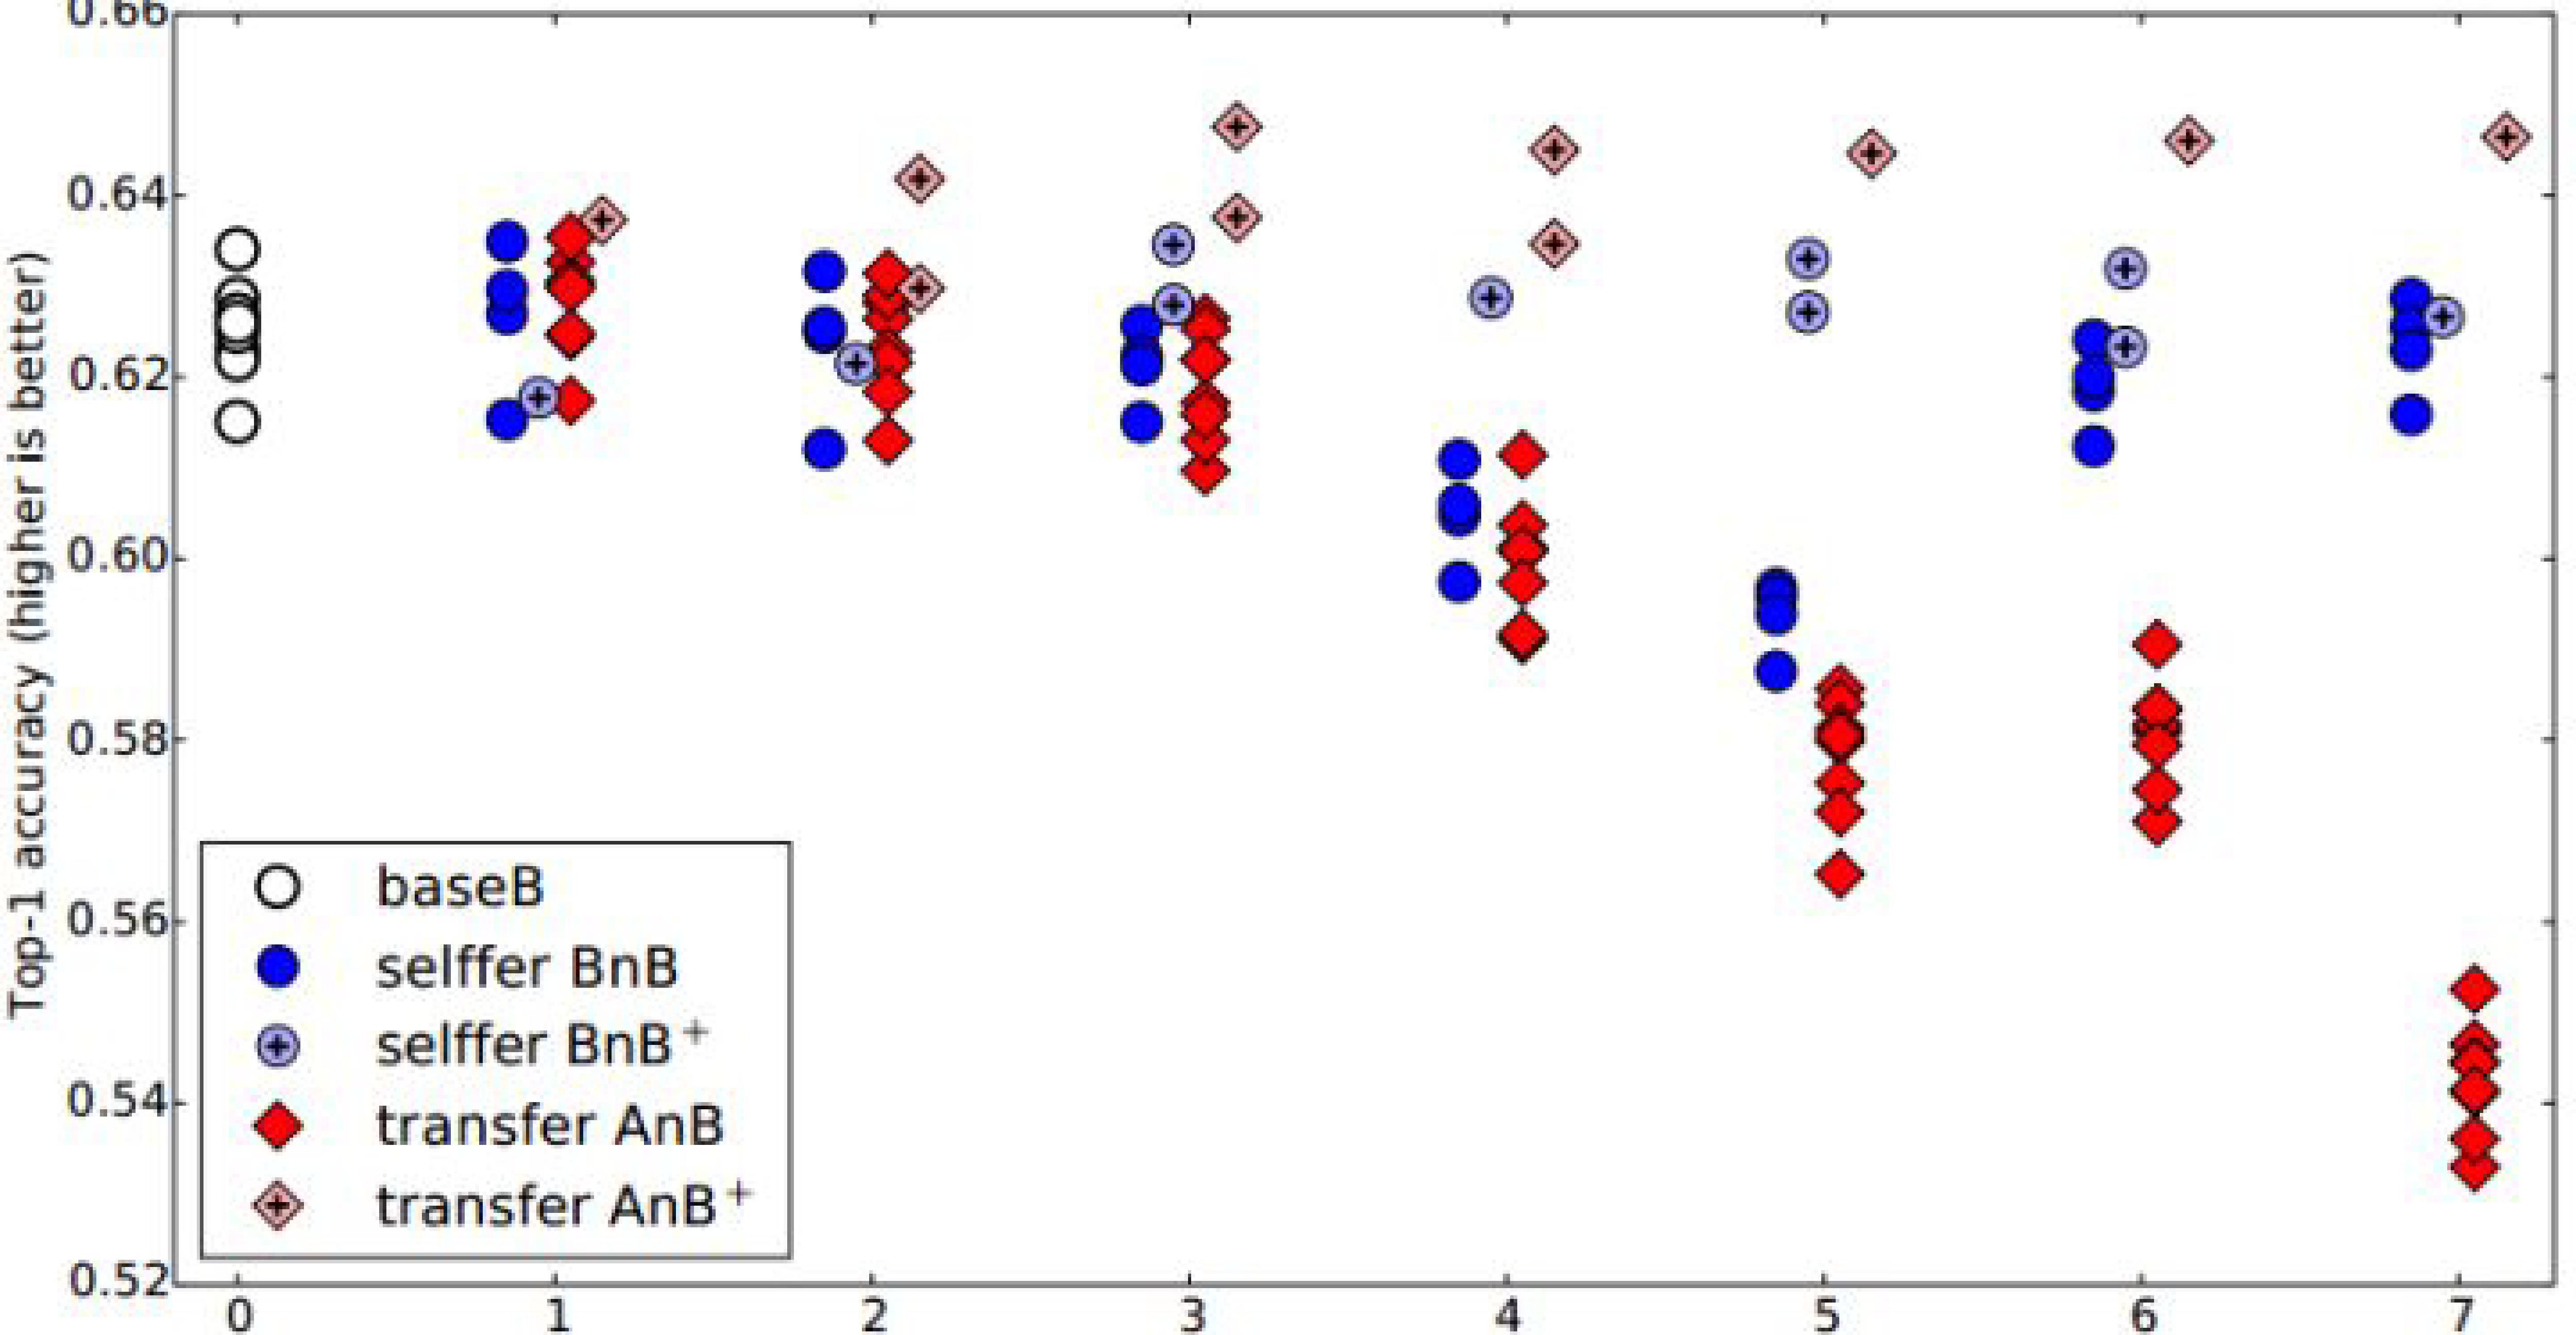
\includegraphics[scale=0.5]{figures/fig-8_1.pdf}
	\caption{深度网络迁移实验结果1}
	\label{fig-8-2}
\end{figure}

这个图说明了什么呢?我们先看蓝色的BnB和BnB+(就是BnB加上finetune)。对BnB而言,原训练好的B模型的前3层直接拿来就可以用而不会对模型精度有什么损失。到了第4和第5层,精度略有下降,不过还是可以接受。然而到了第6第第7层,精度居然奇迹般地回升了!这是为什么?原因如下:对于一开始精度下降的第4第5层来说,确实是到了这一步,feature变得越来越specific,所以下降了。那对于第6第7层为什么精度又不变了?那是因为,整个网络就8层,我们固定了第6第7层,这个网络还能学什么呢?所以很自然地,精度和原来的B网络几乎一致!

对BnB+来说,结果基本上都保持不变。说明finetune对模型结果有着很好的促进作用!

我们重点关注AnB和AnB+。对AnB来说,直接将A网络的前3层迁移到B,貌似不会有什么影响,再一次说明,网络的前3层学到的几乎都是general feature!往后,到了第4第5层的时候,精度开始下降,我们直接说:一定是feature不general了!然而,到了第6第7层,精度出现了小小的提升后又下降,这又是为什么?作者在这里提出两点:co-adaptation和feature representation。就是说,第4第5层精度下降的时候,主要是由于A和B两个数据集的差异比较大,所以会下降;到了第6第7层,由于网络几乎不迭代了,学习能力太差,此时feature学不到,所以精度下降得更厉害。

再看AnB+。加入了finetune以后,AnB+的表现对于所有的$n$几乎都非常好,甚至比baseB(最初的B)还要好一些!这说明:finetune对于深度迁移有着非常好的促进作用!

把上面的结果合并就得到了下面一张图(图~\ref{fig-8-3}):

\begin{figure}[htbp]
	\centering
	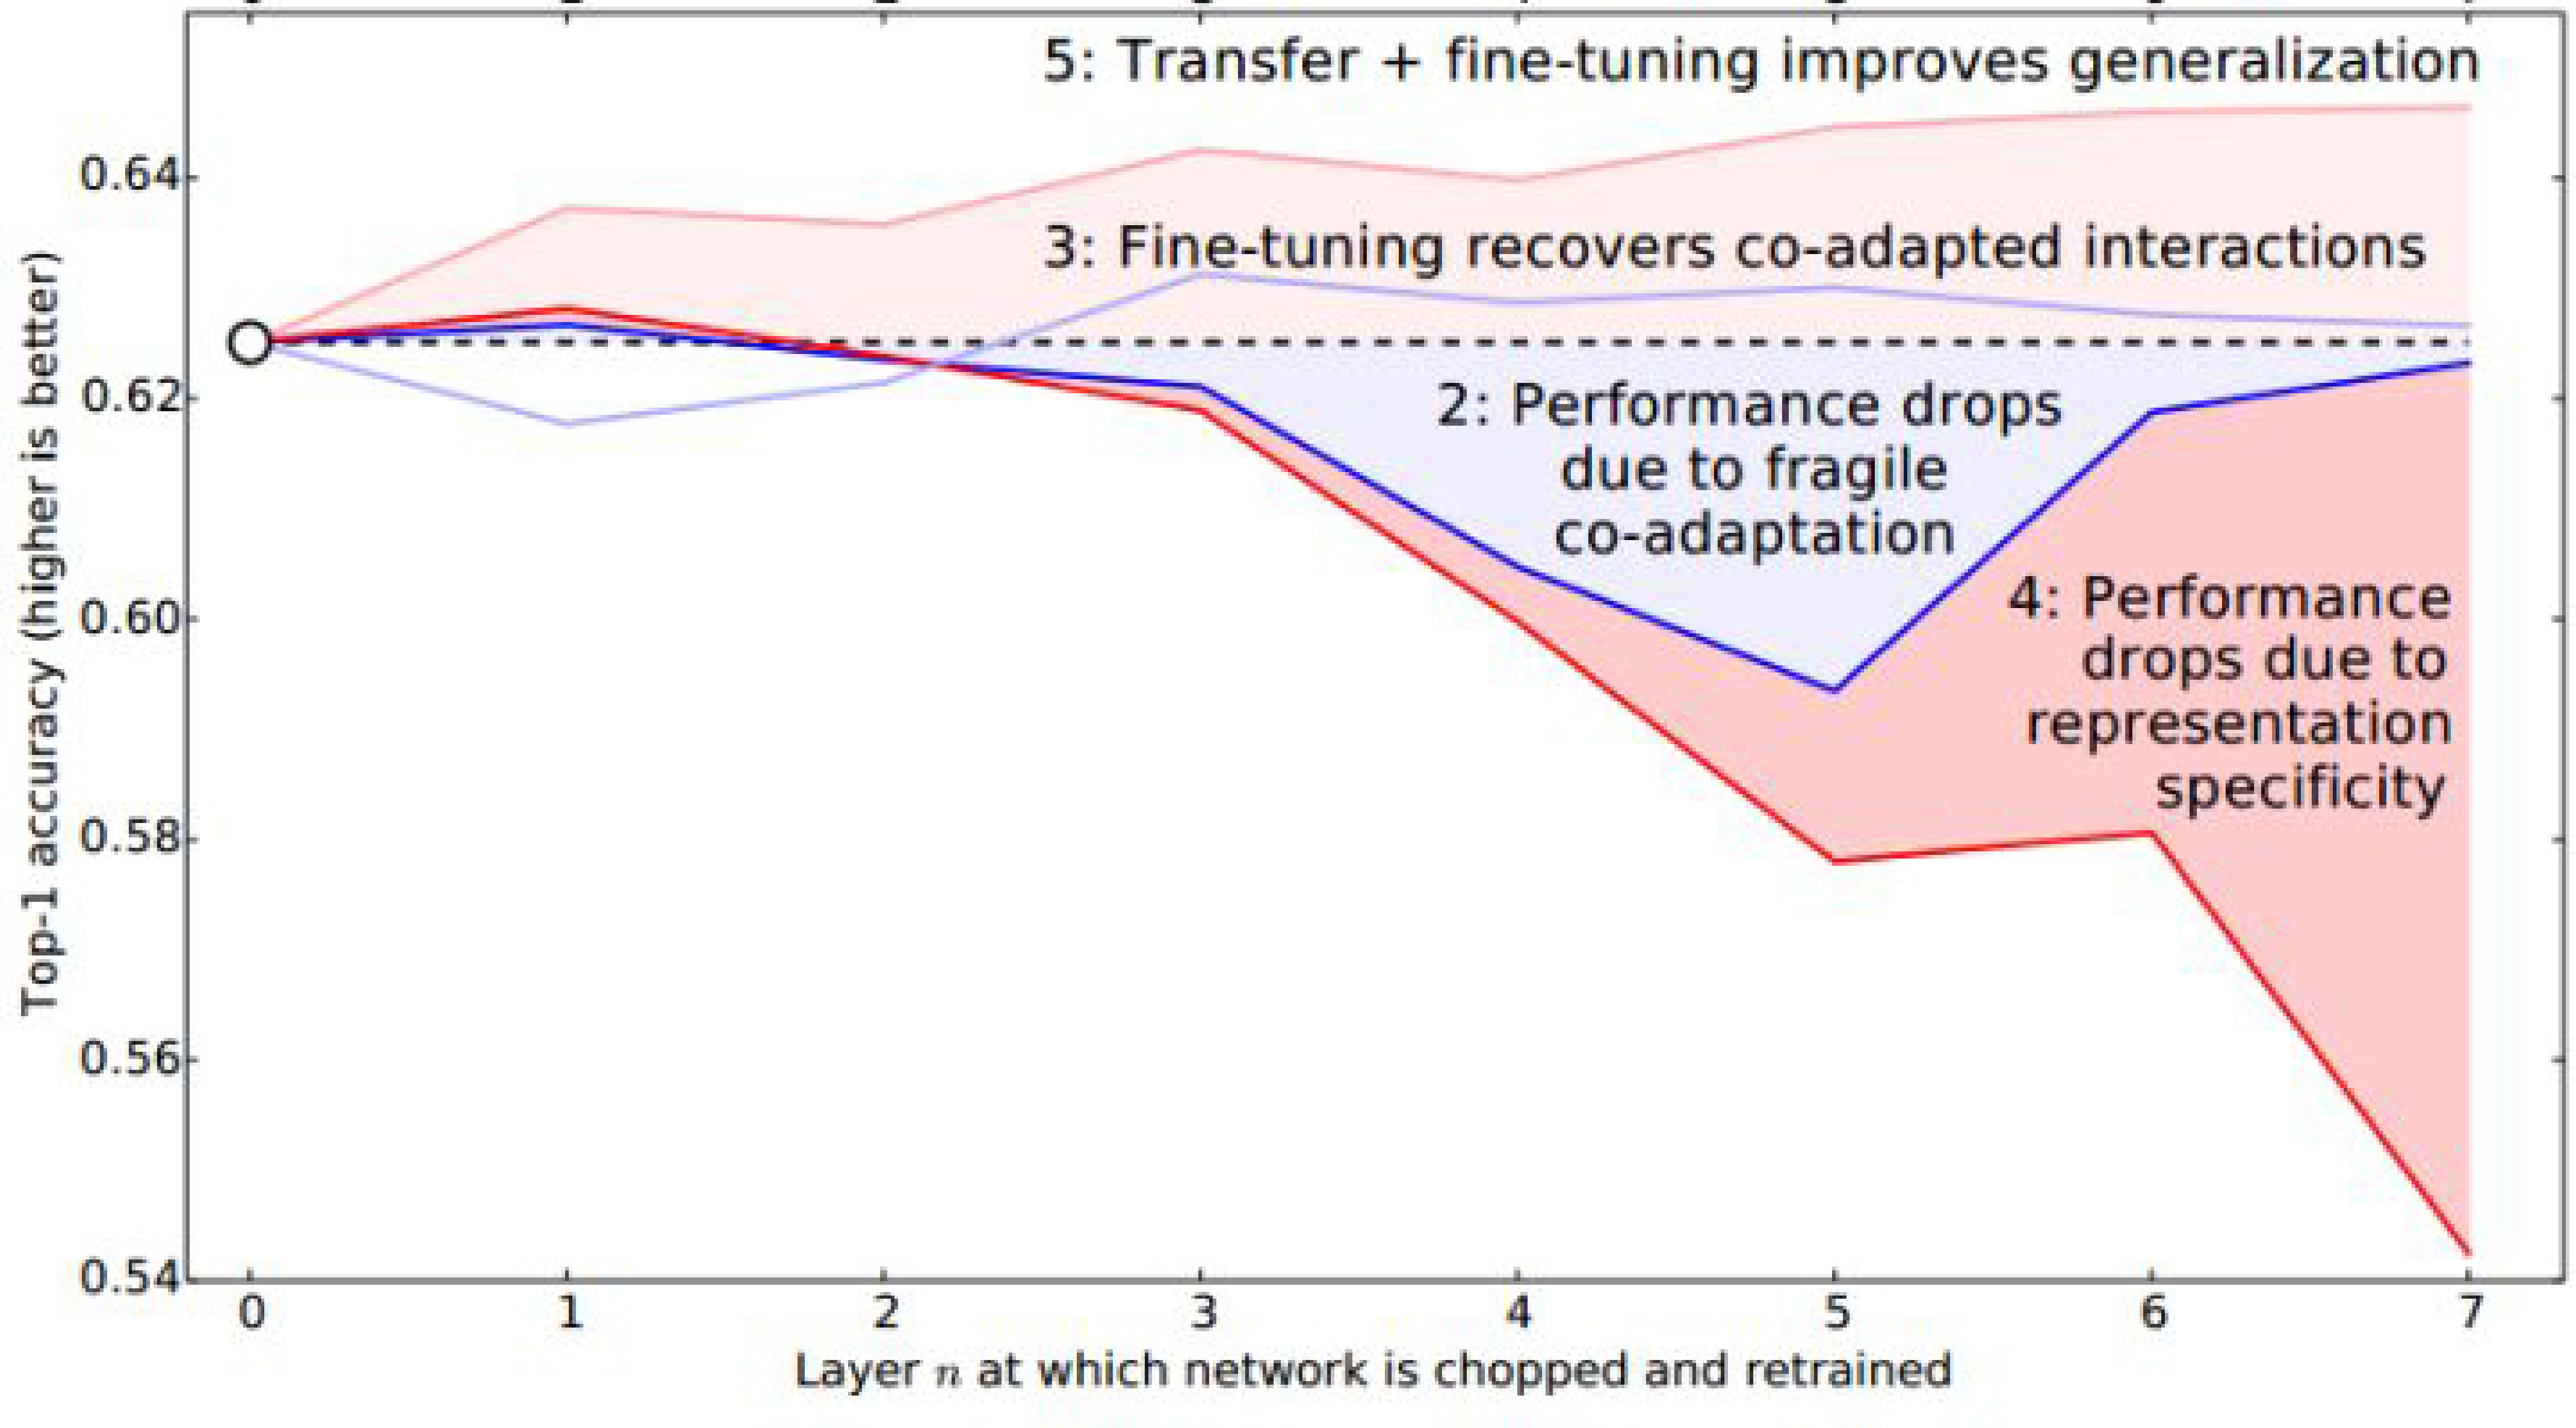
\includegraphics[scale=0.5]{figures/fig-8_2.pdf}
	\caption{深度网络迁移实验结果2}
	\label{fig-8-3}
\end{figure}

至此,AnB和BnB基本完成。作者又想,是不是我分A和B数据的时候,里面存在一些比较相似的类使结果好了?比如说A里有猫,B里有狮子,所以结果会好?为了排除这些影响,作者又分了一下数据集,这次使得A和B里几乎没有相似的类别。在这个条件下再做AnB,与原来精度比较(0\%为基准)得到了下图(图~\ref{fig-8-4}):

\begin{figure}[htbp]
	\centering
	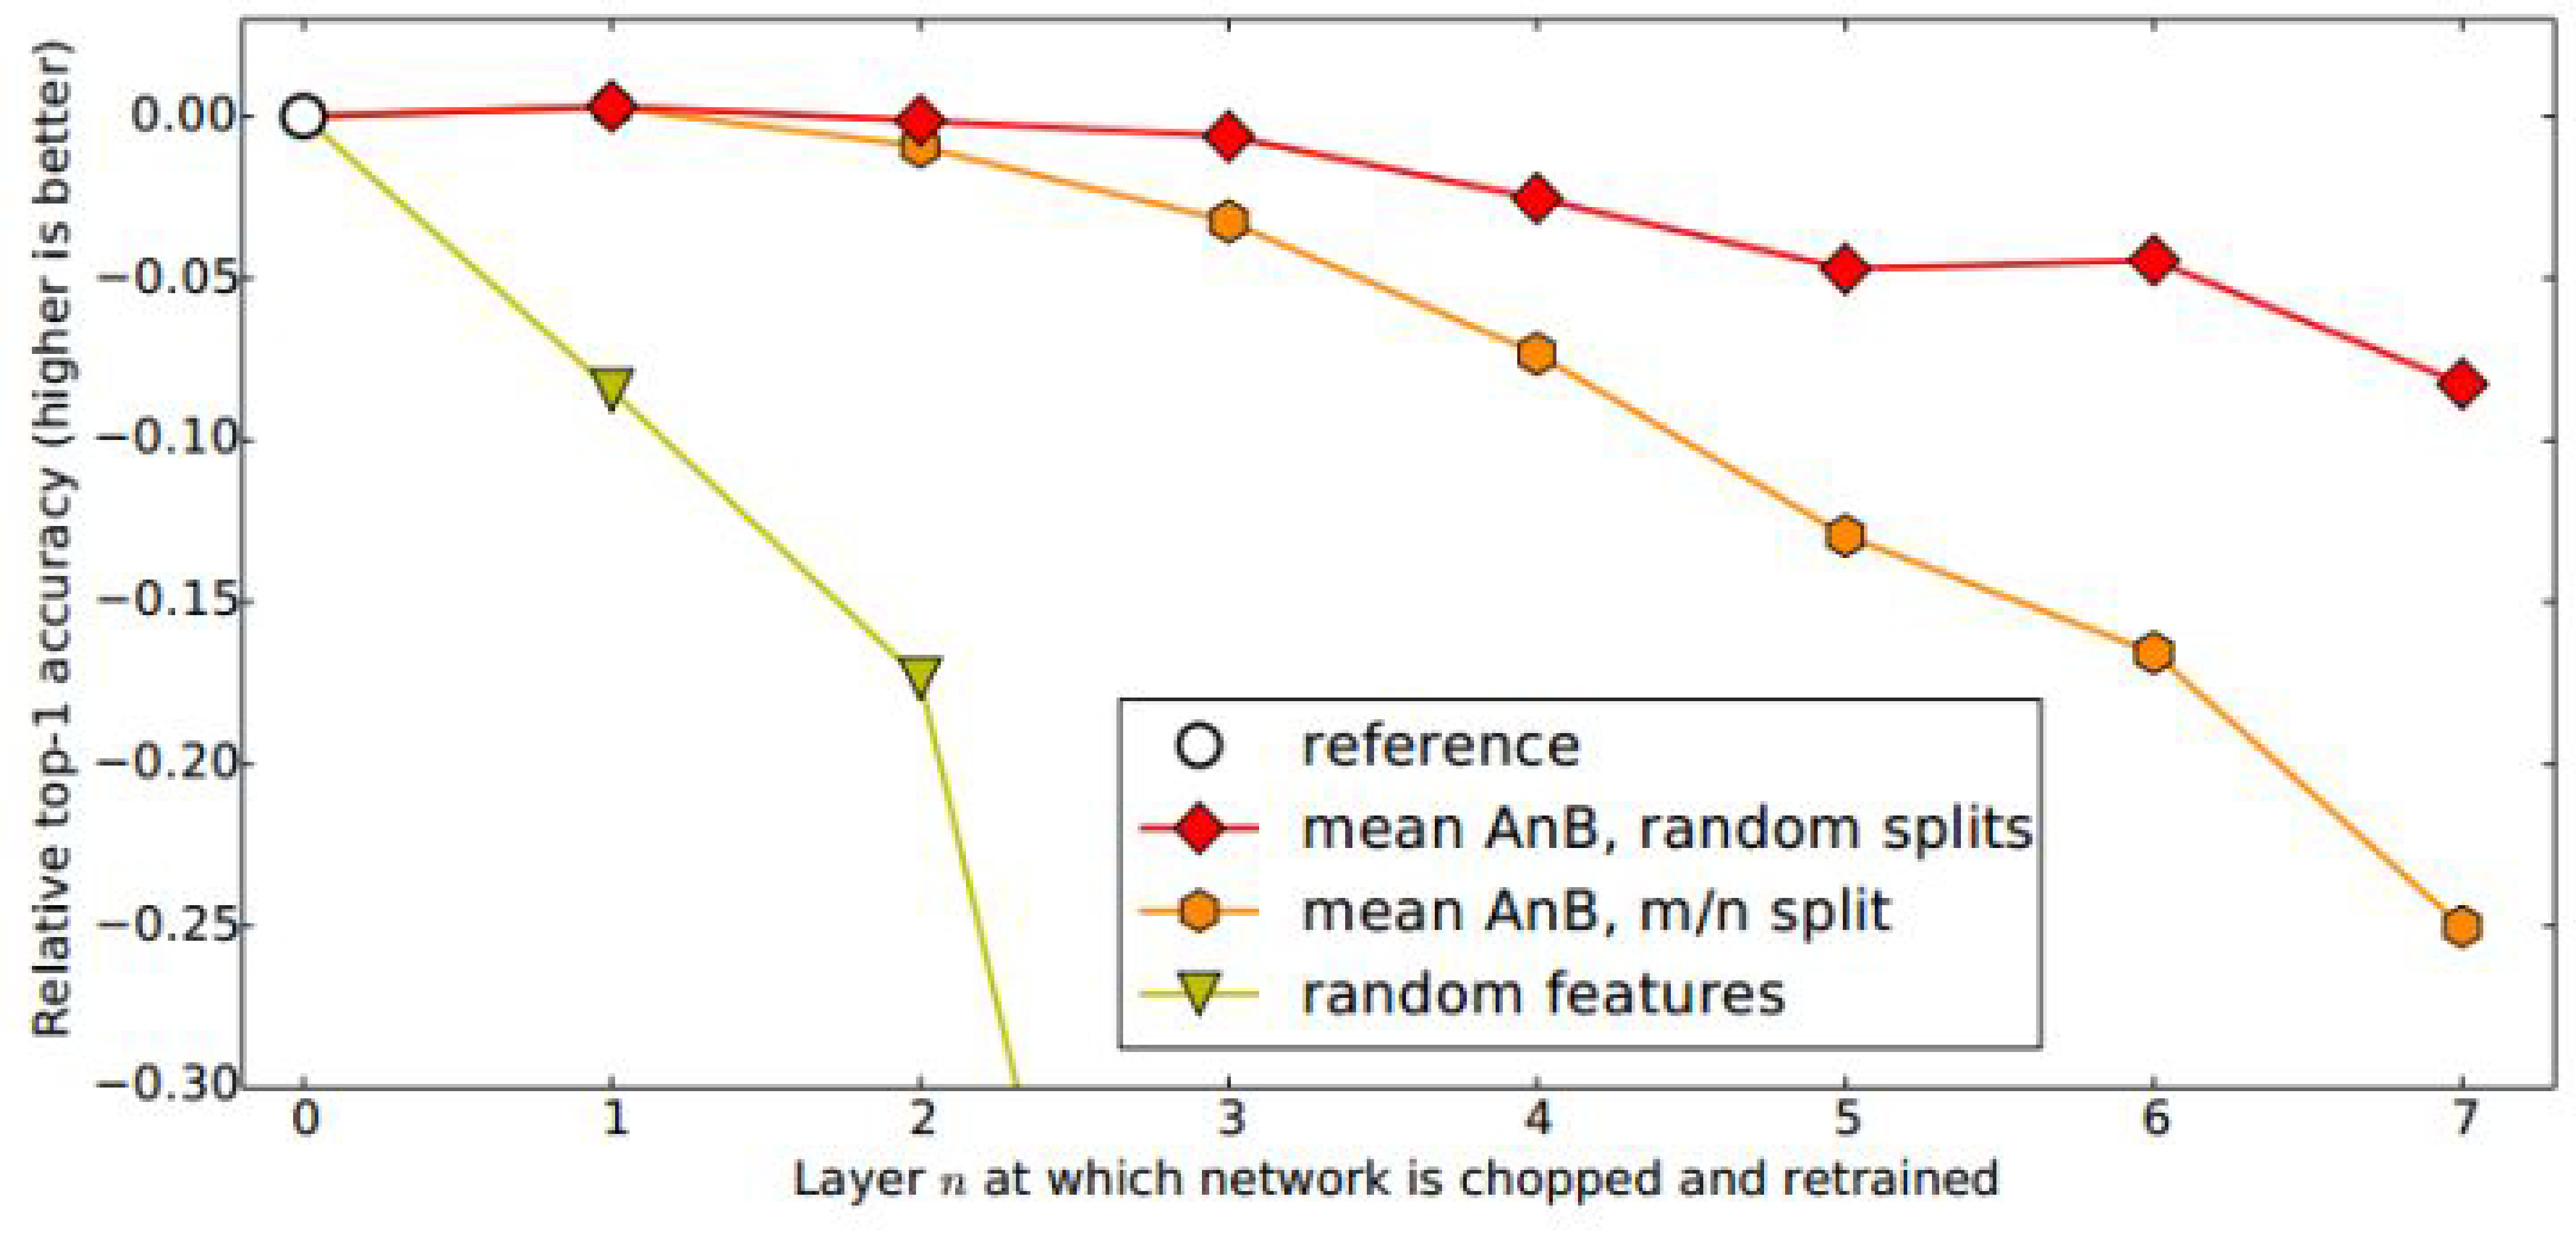
\includegraphics[scale=0.5]{./figures/fig-8_3.pdf}
	\caption{深度网络迁移实验结果3}
	\label{fig-8-4}
\end{figure}

这个图说明了什么呢?简单:随着可迁移层数的增加,模型性能下降。但是,前3层仍然还是可以迁移的!同时,与随机初始化所有权重比较,迁移学习的精度是很高的!

\textbf{结论}

虽然该论文并没有提出一个创新方法,但是通过实验得到了以下几个结论,对以后的深度学习和深度迁移学习都有着非常高的指导意义:

\begin{itemize}
	\item 神经网络的前3层基本都是general feature,进行迁移的效果会比较好;
	\item 深度迁移网络中加入fine-tune,效果会提升比较大,可能会比原网络效果还好;
	\item Fine-tune可以比较好地克服数据之间的差异性;
	\item 深度迁移网络要比随机初始化权重效果好;
	\item 网络层数的迁移可以加速网络的学习和优化。
\end{itemize}

\subsection{最简单的深度迁移:finetune}

深度网络的finetune也许是最简单的深度网络迁移方法。\textbf{Finetune},也叫微调、finetuning,是深度学习中的一个重要概念。简而言之,finetune就是利用别人已经训练好的网络,针对自己的任务再进行调整。从这个意思上看,我们不难理解finetune是迁移学习的一部分。

\textbf{1. 为什么需要已经训练好的网络?}

在实际的应用中,我们通常不会针对一个新任务,就去从头开始训练一个神经网络。这样的操作显然是非常耗时的。尤其是,我们的训练数据不可能像ImageNet那么大,可以训练出泛化能力足够强的深度神经网络。即使有如此之多的训练数据,我们从头开始训练,其代价也是不可承受的。

那么怎么办呢?迁移学习告诉我们,利用之前已经训练好的模型,将它很好地迁移到自己的任务上即可。

\textbf{2. 为什么需要finetune?}

因为别人训练好的模型,可能\textit{并不是完全适用}于我们自己的任务。可能别人的训练数据和我们的数据之间不服从同一个分布;可能别人的网络能做比我们的任务更多的事情;可能别人的网络比较复杂,我们的任务比较简单。

举一个例子来说,假如我们想训练一个猫狗图像二分类的神经网络,那么很有参考价值的就是在CIFAR-100上训练好的神经网络。但是CIFAR-100有100个类别,我们只需要2个类别。此时,就需要针对我们自己的任务,固定原始网络的相关层,修改网络的输出层,以使结果更符合我们的需要。

图~\ref{fig-deep-finetune}展示了一个简单的finetune过程。从图中我们可以看到,我们采用的预训练好的网络非常复杂,如果直接拿来从头开始训练,则时间成本会非常高昂。我们可以将此网络进行改造,固定前面若干层的参数,只针对我们的任务,微调后面若干层。这样,网络训练速度会极大地加快,而且对提高我们任务的表现也具有很大的促进作用。

\begin{figure}[htbp]
	\centering
	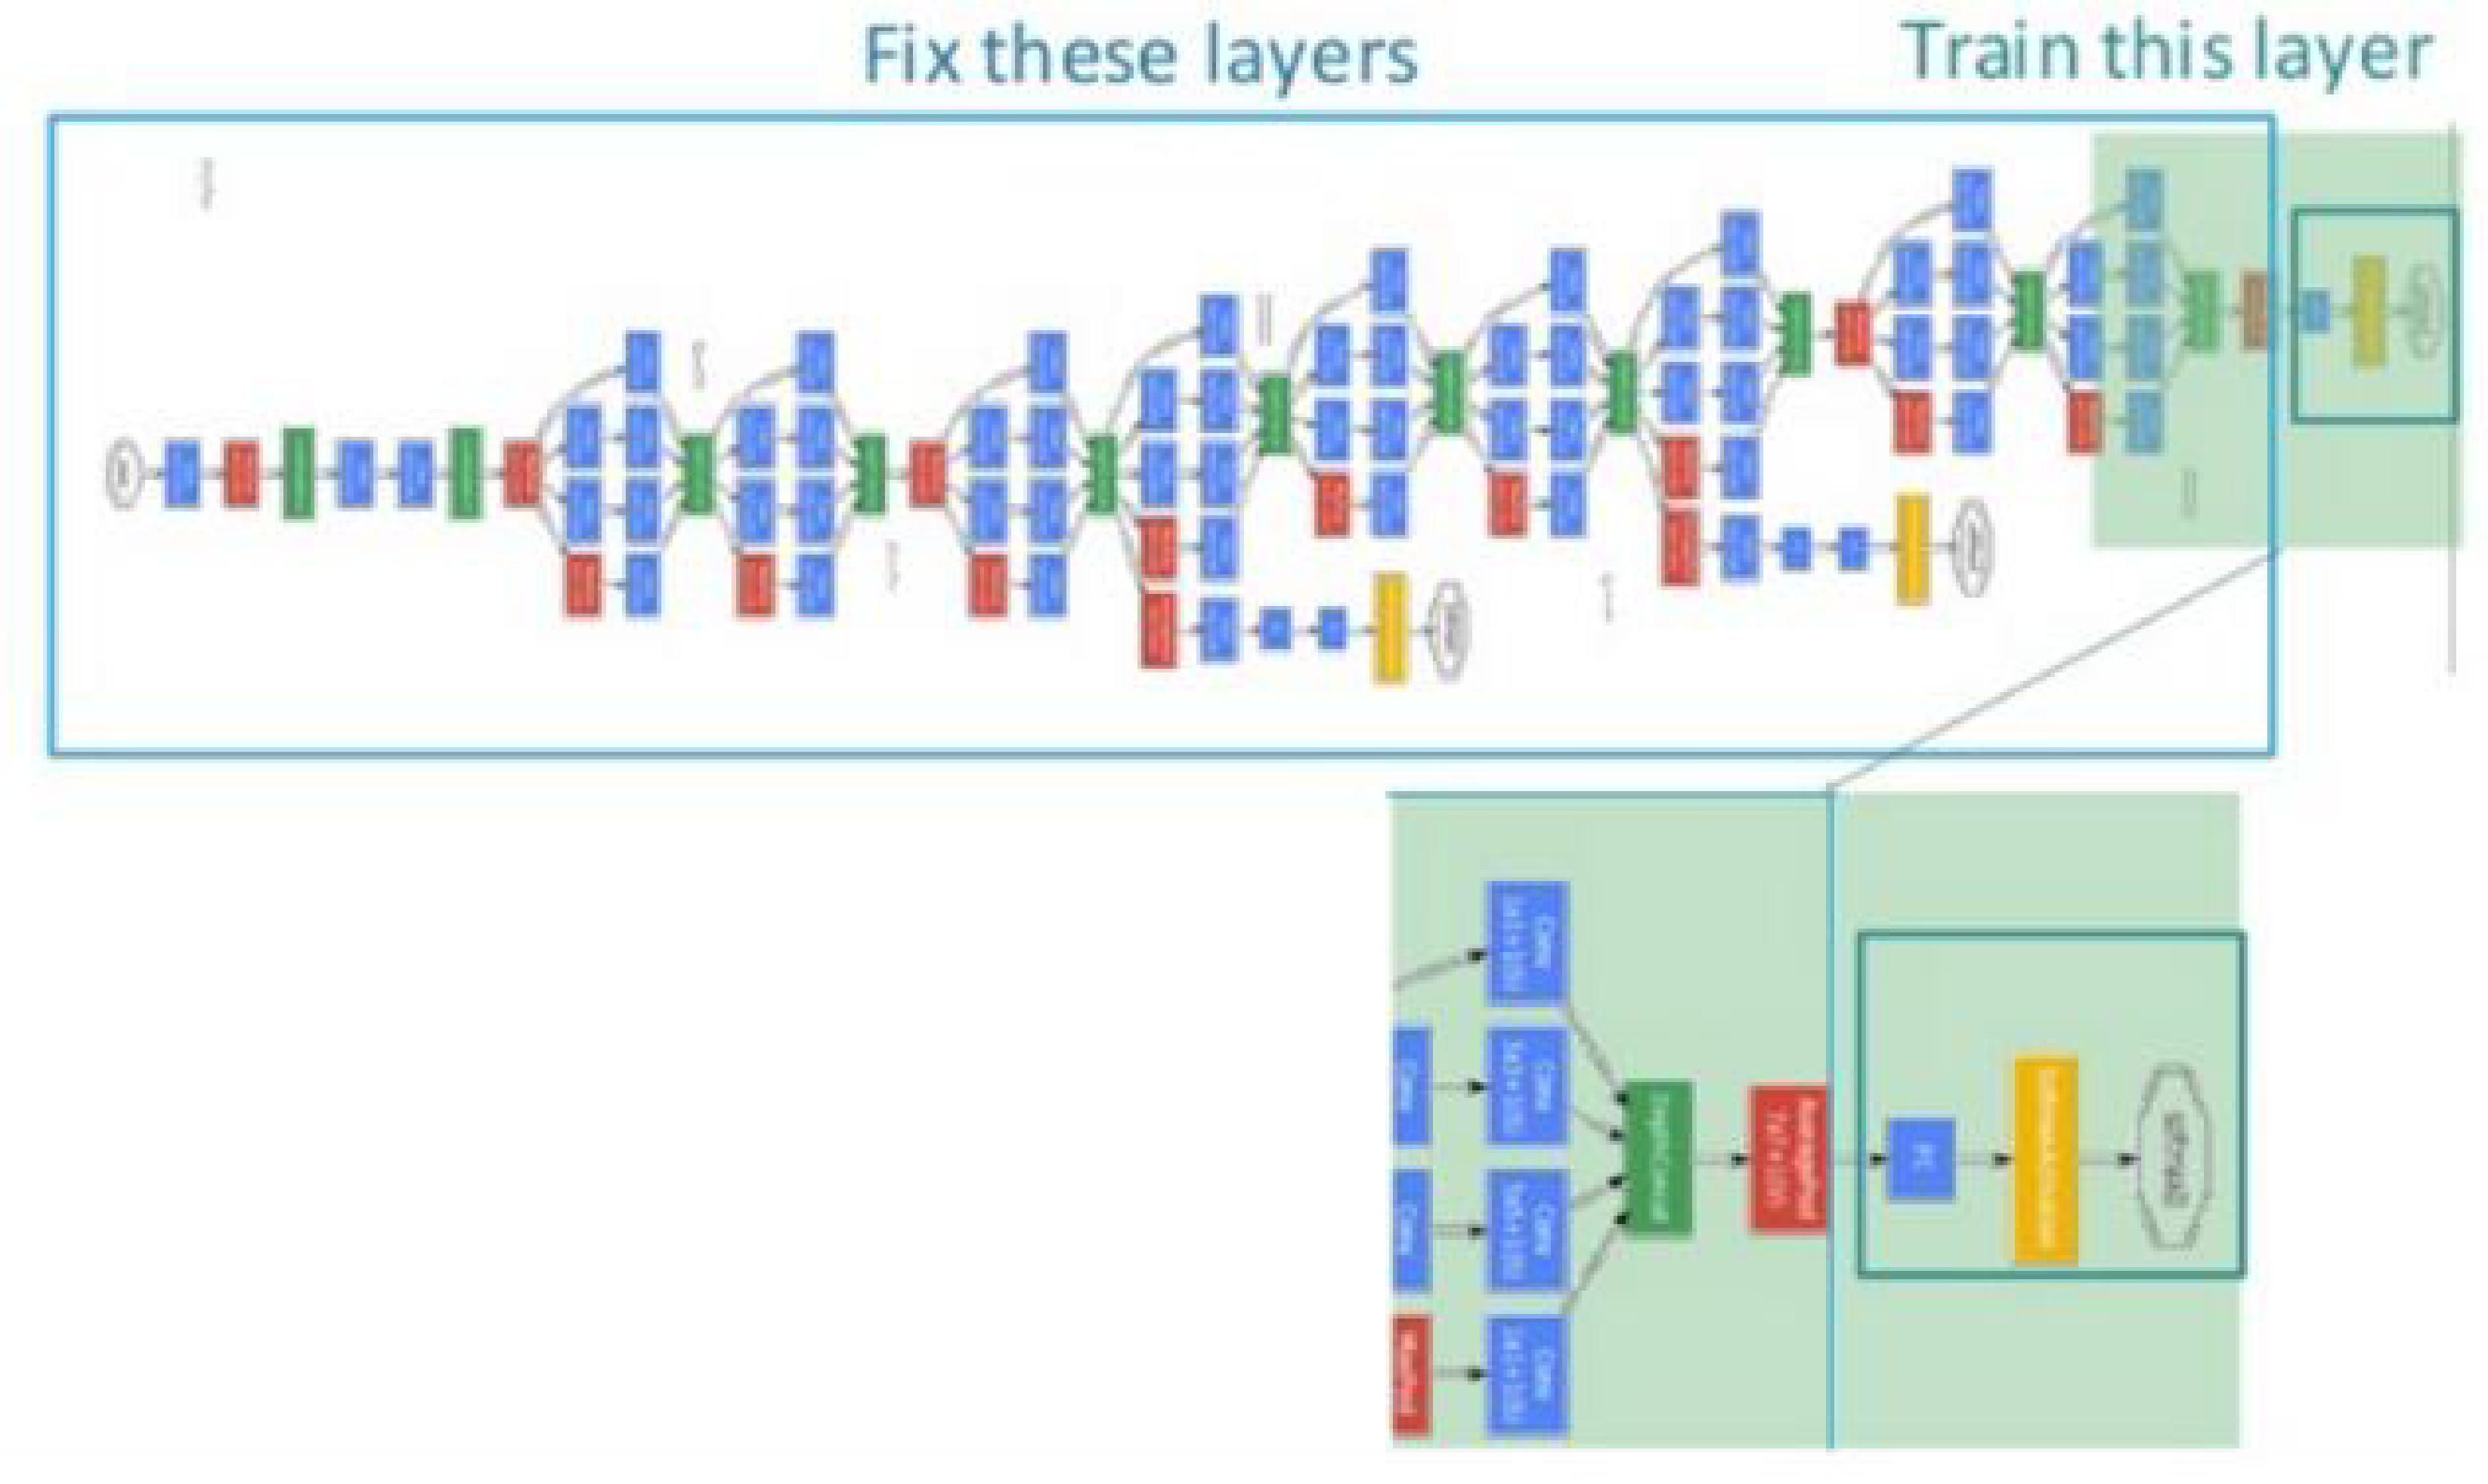
\includegraphics[scale=0.6]{./figures/fig-deep-finetune.pdf}
	\caption{一个简单的finetune示意图}
	\label{fig-deep-finetune}
\end{figure}

\textbf{3. Finetune的优势}

Finetune的优势是显然的,包括:

\begin{itemize}
	\item 不需要针对新任务从头开始训练网络,节省了时间成本;
	\item 预训练好的模型通常都是在大数据集上进行的,无形中扩充了我们的训练数据,使得模型更鲁棒、泛化能力更好;
	\item Finetune实现简单,使得我们只关注自己的任务即可。
\end{itemize}

\textbf{4. Finetune的扩展}

在实际应用中,通常几乎没有人会针对自己的新任务从头开始训练一个神经网络。Finetune是一个理想的选择。

Finetune并不只是针对深度神经网络有促进作用,对传统的非深度学习也有很好的效果。例如,finetune对传统的人工提取特征方法就进行了很好的替代。我们可以使用深度网络对原始数据进行训练,依赖网络提取出更丰富更有表现力的特征。然后,将这些特征作为传统机器学习方法的输入。这样的好处是显然的:\textit{既避免了繁复的手工特征提取,又能自动地提取出更有表现力的特征。}

比如,图像领域的研究,一直是以SIFT、SURF等传统特征为依据的,直到2014年,伯克利的研究人员提出了DeCAF特征提取方法~\cite{donahue2014decaf},直接使用深度卷积神经网络进行特征提取。实验结果表明,该特征提取方法对比传统的图像特征,在精度上有着无可匹敌的优势。另外,也有研究人员用卷积神经网络提取的特征作为SVM分类器的输入~\cite{razavian2014cnn},显著提升了图像分类的精度。

\subsection{深度网络自适应}

\subsubsection{基本思路}

深度网络的finetune可以帮助我们节省训练时间,提高学习精度。但是finetune有它的先天不足:它无法处理训练数据和测试数据分布不同的情况。而这一现象在实际应用中比比皆是。因为finetune的基本假设也是训练数据和测试数据服从相同的数据分布。这在迁移学习中也是不成立的。因此,我们需要更进一步,针对深度网络开发出更好的方法使之更好地完成迁移学习任务。

以我们之前介绍过的数据分布自适应方法为参考,许多深度学习方法~\cite{tzeng2014deep,long2015learning}都开发出了\textit{自适应层}(Adaptation Layer)来完成源域和目标域数据的自适应。自适应能够使得源域和目标域的数据分布更加接近,从而使得网络的效果更好。

从上述的分析我们可以得出,深度网络的自适应主要完成两部分的工作:

一是哪些层可以自适应,这决定了网络的学习程度;

二是采用什么样的自适应方法(度量准则),这决定了网络的泛化能力。

深度网络中最重要的是网络损失的定义。绝大多数深度迁移学习方法都采用了以下的损失定义方式:

\begin{equation}
	\ell = \ell_c(\mathcal{D}_s,\mathbf{y}_s) + \lambda \ell_A(\mathcal{D}_s,\mathcal{D}_t)
\end{equation}

其中,$\ell$表示网络的最终损失,$\ell_c(\mathcal{D}_s,\mathbf{y}_s)$表示网络在有标注的数据(大部分是源域)上的常规分类损失(这与普通的深度网络完全一致),$\ell_A(\mathcal{D}_s,\mathcal{D}_t)$表示网络的自适应损失。最后一部分是传统的深度网络所不具有的、迁移学习所独有的。此部分的表达与我们先前讨论过的源域和目标域的分布差异,在道理上是相同的。式中的$\lambda$是权衡两部分的权重参数。

上述的分析指导我们设计深度迁移网络的基本准则:决定自适应层,然后在这些层加入自适应度量,最后对网络进行finetune。

\subsubsection{核心方法}

前期的研究者在2014年环太平洋人工智能大会(PRICAI)上提出了一个叫做DaNN(Domain Adaptive Neural Network)的神经网络~\cite{ghifary2014domain}。DaNN的结构异常简单,它仅由两层神经元组成:特征层和分类器层。作者的创新工作在于,在特征层后加入了一项MMD适配层,用来计算源域和目标域的距离,并将其加入网络的损失中进行训练。

但是,由于网络太浅,表征能力有限,故无法很有效地解决domain adaptation问题。因此,后续的研究者大多数都基于其思想进行扩充,如将浅层网络改为更深层的AlexNet、ResNet、VGG等;如将MMD换为多核的MMD等。

\textbf{1. 第一个方法:DDC}

加州大学伯克利分校的Tzeng等人~\cite{tzeng2014deep}首先提出了一个DDC方法(Deep Domain Confusion)解决深度网络的自适应问题。DDC遵循了我们上述讨论过的基本思路,采用了在ImageNet数据集上训练好的AlexNet网络~\cite{krizhevsky2012imagenet}进行自适应学习。

图~\ref{fig-deep-ddc}是DDC方法的示意。DDC固定了AlexNet的前7层,在第8层(分类器前一层)上加入了自适应的度量。自适应度量方法采用了被广泛使用的MMD准则。DDC方法的损失函数表示为:

\begin{equation}
	\label{eq-deep-ddc}
	\ell = \ell_c(\mathcal{D}_s,\mathbf{y}_s) + \lambda MMD^2(\mathcal{D}_s,\mathcal{D}_t)
\end{equation}

\begin{figure}[htbp]
	\centering
	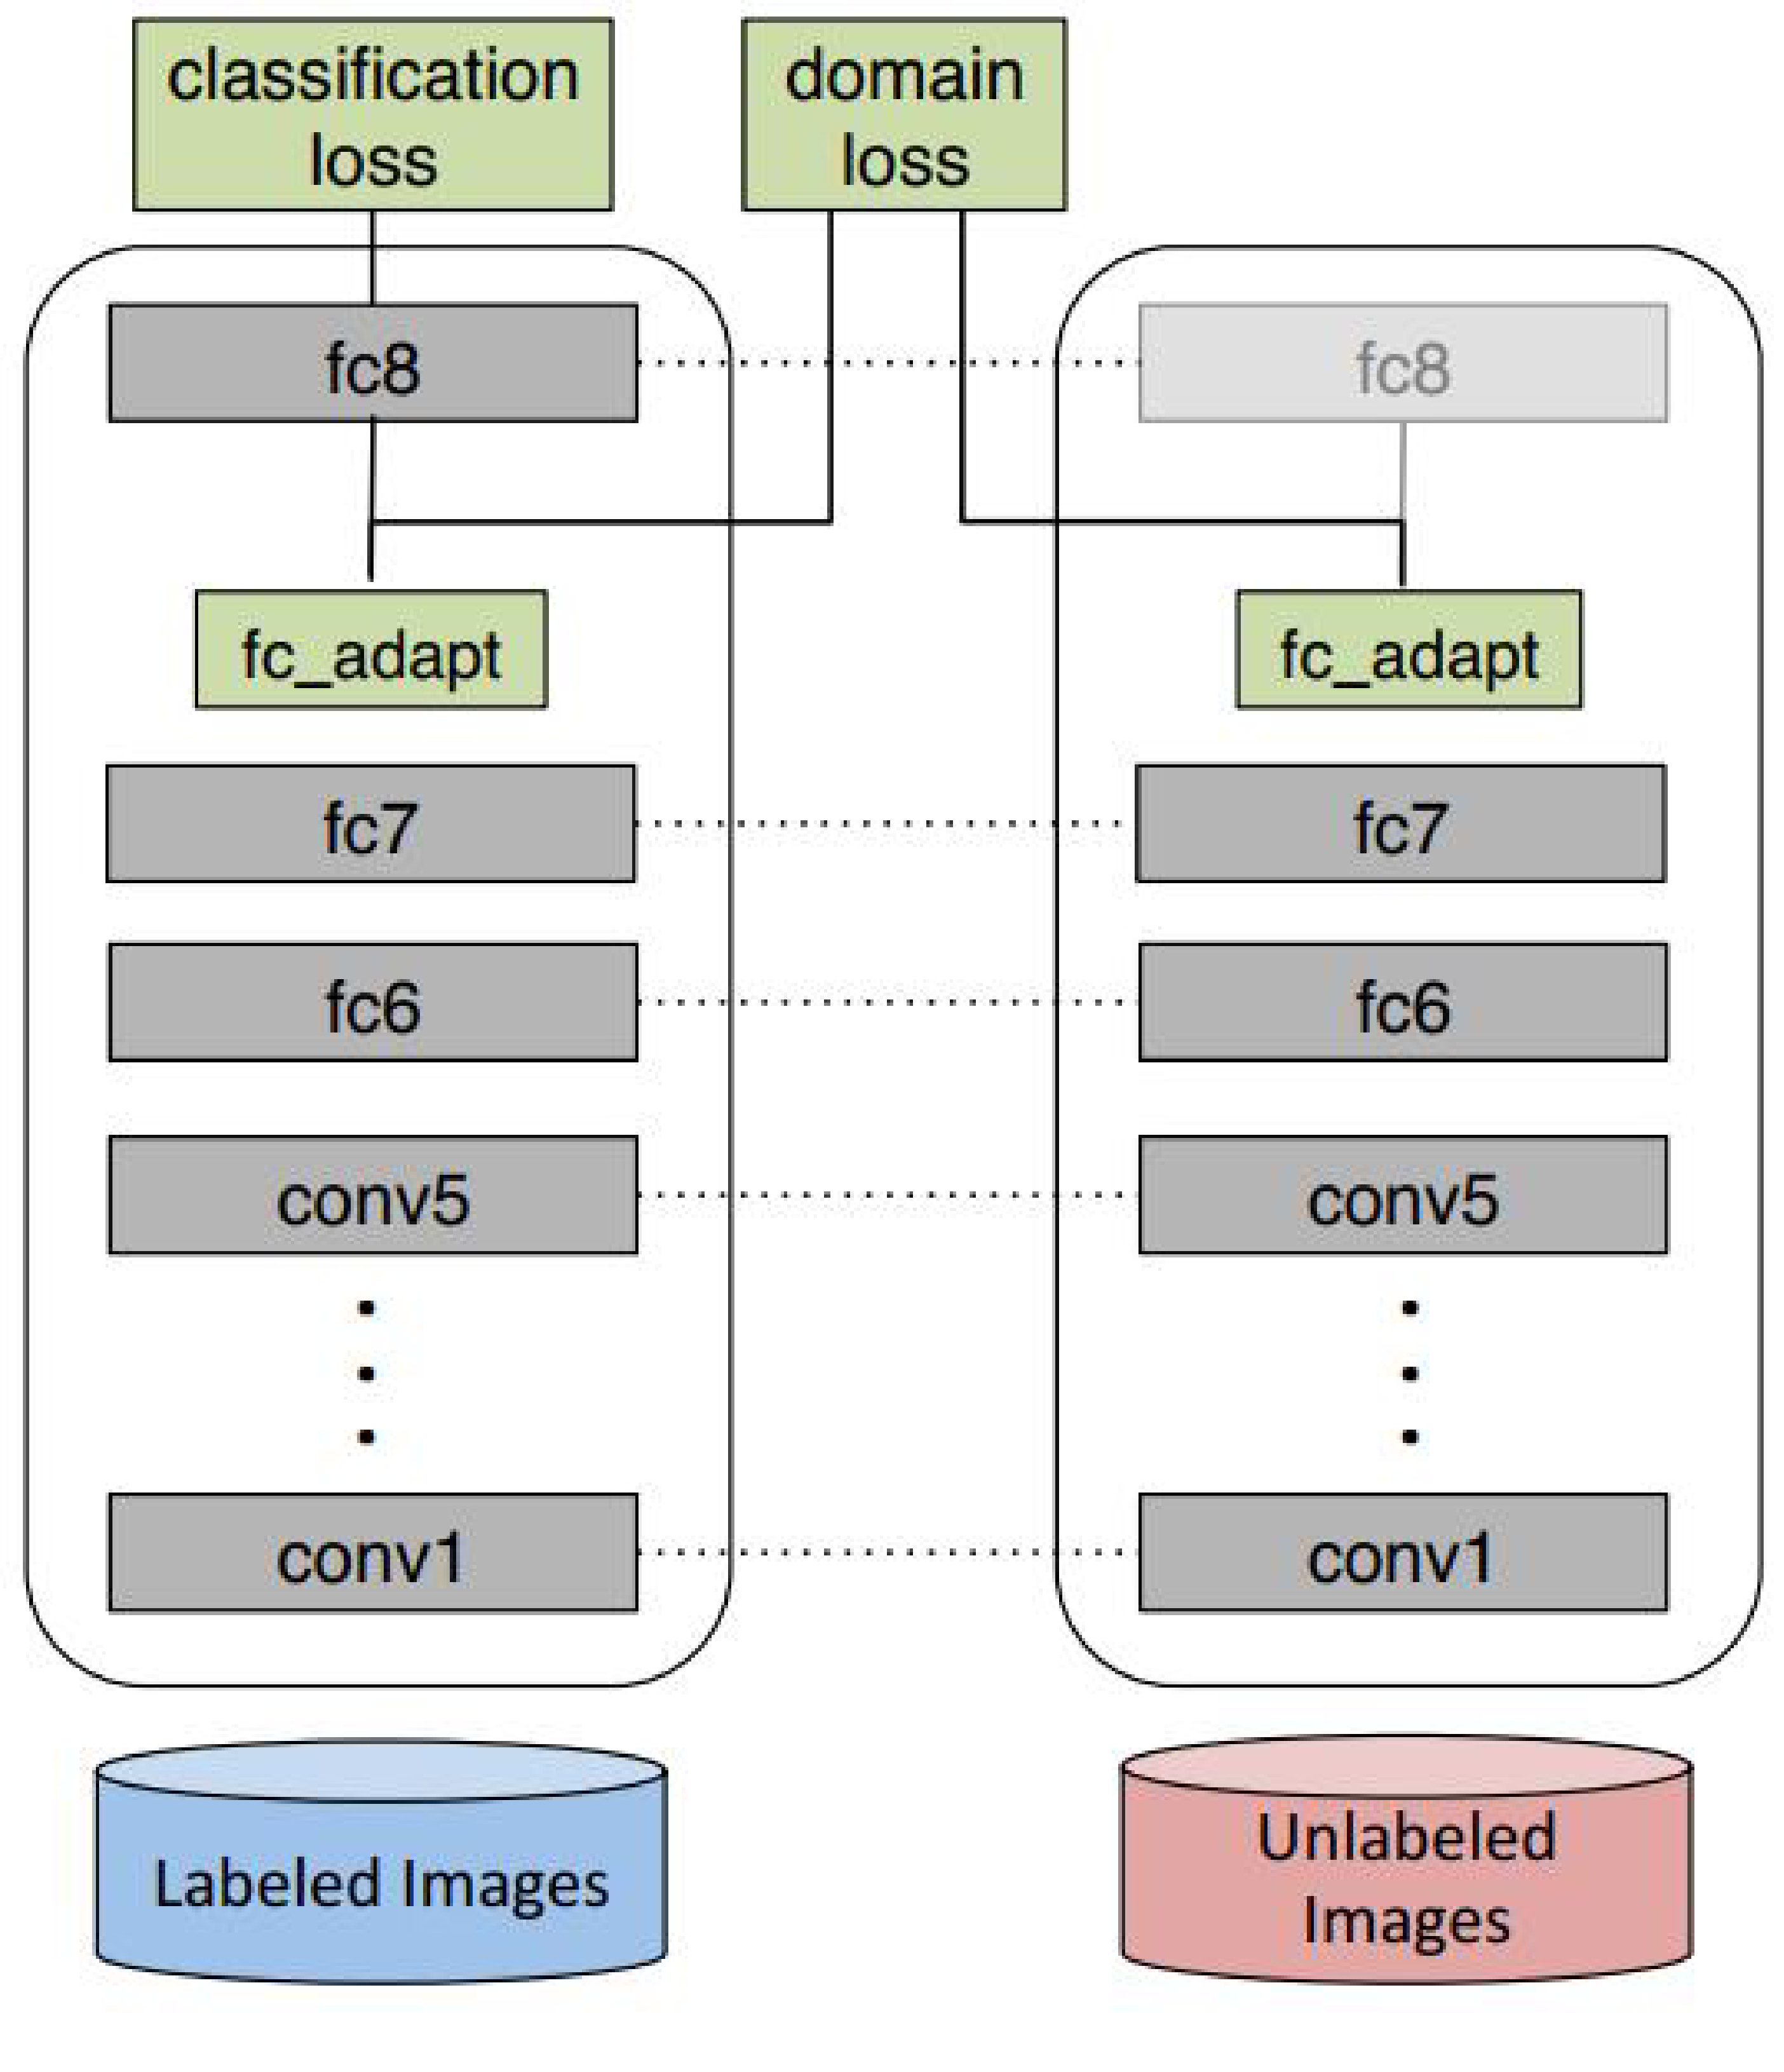
\includegraphics[scale=0.6]{./figures/fig-deep-ddc.pdf}
	\caption{DDC方法示意图}
	\label{fig-deep-ddc}
\end{figure}

\textbf{为什么选择了倒数第二层?} DDC方法的作者在文章中提到,他们经过了多次实验,在不同的层进行了尝试,最终得出结论,在分类器前一层加入自适应可以达到最好的效果。

这也是与我们的认知相符合的。通常来说,分类器前一层即特征,在特征上加入自适应,也正是迁移学习要完成的工作。

\textbf{2. DAN}

来自清华大学的龙明盛等人在2015年发表在机器学习顶级会议ICML上的DAN方法(Deep Adaptation Networks)~\cite{long2015learning}对DDC方法进行了几个方面的扩展。首先,有别于DDC方法只加入一个自适应层,DAN方法同时加入了三个自适应层(分类器前三层)。其次,DAN方法采用了表征能力更好的多核MMD度量(MK-MMD)~\cite{gretton2012optimal}代替了DDC方法中的单一核MMD。然后,DAN方法将多核MMD的参数学习融入到深度网络的训练中,不增加网络的额外训练时间。DAN方法在多个任务上都取得了比DDC更好的分类效果。

为什么是适配3层?原来的DDC方法只是适配了一层,现在DAN也基于AlexNet网络,适配最后三层(第6第7第8层)。为什么是这三层?因为在Jason的文章~\cite{yosinski2014transferable}中已经说了,网络的迁移能力在这三层开始就会特别地task-specific,所以要着重适配这三层。至于别的网络(比如GoogLeNet、VGG)等是不是这三层就需要通过自己的实验来推测。DAN只关注使用AlexNet。

MK-MMD的多核表示形式为

\begin{equation}
	\mathcal{K} \triangleq \left\{k= \sum_{u=1}^{m}\beta_u k_u : \beta_u \ge 0, \forall u \right\}
\end{equation}

DAN的优化目标也由两部分组成:损失函数和自适应损失。损失函数这个好理解,基本上所有的机器学习方法都会定义一个损失函数,它来度量预测值和真实值的差异。分布距离就是我们上面提到的MK-MMD距离。于是,DAN的优化目标就是

\begin{equation}
	\label{eq-deep-dan}
	\min_\Theta \frac{1}{n_a} \sum_{i=1}^{n_a} J(\theta(\mathbf{x}^a_i),y^a_i) + \lambda \sum_{l=l_1}^{l_2}d^2_k(\mathcal{D}^l_s,\mathcal{D}^l_t)
\end{equation}

这个式子中,$\Theta$表示网络的所有权重和bias参数,是用来学习的目标。其中$l_1,l_2$分别是6和8,表示网络适配是从第6层到第8层,前面的不进行适配。$\mathbf{x}_a,n_a$表示源域和目标域中所有有标注的数据的集合。$J(\cdot)$就定义了一个损失函数,在深度网络中一般都是cross-entropy。DAN的网络结构如下图所示。

\begin{figure}[htbp]
	\centering
	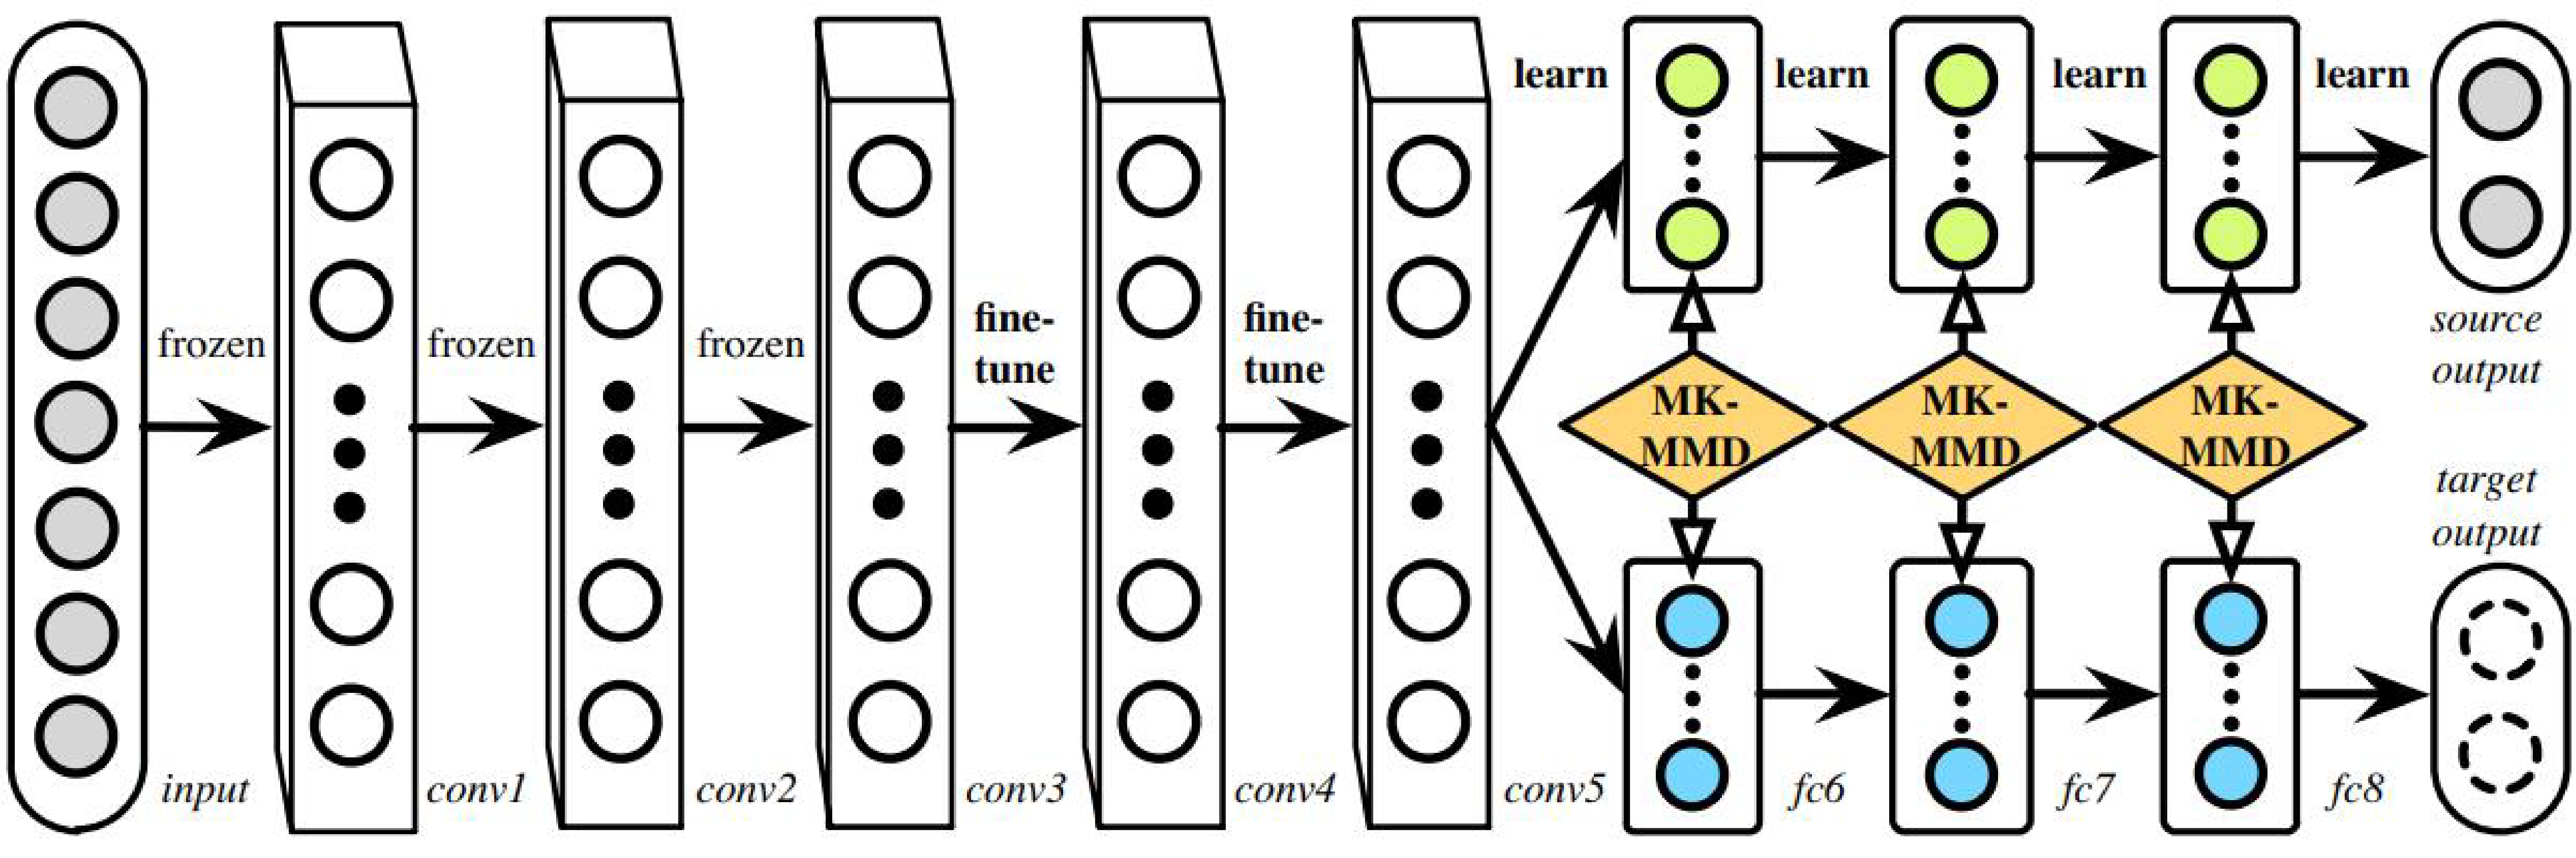
\includegraphics[scale=0.45]{./figures/fig-deep-dan.pdf}
	\caption{DAN方法示意图}
	\label{fig-deep-dan}
\end{figure}

\textbf{学习策略}

DAN的学习一共分为两大类参数:学习网络参数$\Theta$和MMD的$\beta$。

对$\Theta$的学习依赖于MK-MMD距离的计算。通过kernel trick(类比以前的MMD变换)我们总是可以把MK-MMD展开成一堆内积的形式。然而,数据之间两两计算内积是非常复杂的,时间复杂度为$O(n^2)$,这个在深度学习中的开销非常之大。怎么办?作者在这里采用了Gretton在文章~\cite{gretton2012optimal}提出的对MK-MMD的无偏估计:$d^2_k(p,q)=\frac{2}{n_s}\sum_{i=1}^{n_s/2}g_k(\mathbf{z}_i)$,其中的$\mathbf{z}_i$是一个四元组:$\mathbf{z}_i \triangleq (\mathbf{x}^s_{2i-1},\mathbf{x}^s_{2i},\mathbf{x}^t_{2i-1},\mathbf{x}^t_{2i})$。将kernel作用到$\mathbf{z}_i$上以后,变成$g_k(\mathbf{z}_i) \triangleq k(\mathbf{x}^s_{2i-1},\mathbf{x}^s_{2i})+k(\mathbf{x}^t_{2i-1},\mathbf{x}^t_{2i})-k(\mathbf{x}^s_{2i-1},\mathbf{x}^t_{2i})-k(\mathbf{x}^s_{2i},\mathbf{x}^t_{2i-1})$。

上面这些变换看着很复杂。简单来说,它就是只计算了连续的一对数据的距离,再乘以2.这样就可以把时间复杂度降低到$O(n)$!至于具体的理论,可以去参考Gretton的论文,这里就不说了。

在具体进行SGD的时候,我们需要对所有的参数求导:对$\Theta$求导。在实际用multiple-kernel的时候,作者用的是多个高斯核。

学习$\beta$主要是为了确定多个kernel的权重。学习的时候,目标是:确保每个kernel生成的MMD距离的方差最小。也就是

\begin{equation}
	\max_{k \in \mathcal{K}} d^2_k(\mathcal{D}^l_s,\mathcal{D}^l_t) \sigma^{-2}_k
\end{equation}

这里的$\sigma^{-2}_k=E[g^2_k(\mathbf{z})]-[E(g_k(\mathbf{z}))]^2$是估计方差。实际求解的时候问题可以被规约成一个二次规划问题求解,具体可以参照文章。

\textbf{3. 同时迁移领域和任务}

DDC的作者Tzeng在2015年扩展了DDC方法,提出了领域和任务同时迁移的方法~\cite{tzeng2015simultaneous}。作者提出网络要进行两部分的迁移:

一是domain transfer,就是适配分布,特别地是指适配marginal distribution,但是没有考虑类别信息。如何做domain transfer:在传统深度网路的loss上,再加另一个confusion loss,作为classifier能否将两个domain进行分开的loss。两个loss一起计算,就是domain transfer。

二是task transfer,就是利用class之间的相似度,其实特指的是conditional distribution。类别之间有相似度,要利用上。类别之间的相似度:比如一个杯子与瓶子更相似,而与键盘不相似。文章的原话:it does not necessarily align the classes in the target with those in the source. Thus, we also explicity transfer the similarity structure amongst categories.

现有的深度迁移学习方法通常都只是考虑domain transfer,\textit{而没有考虑到类别之间的信息}。如何把domain和task transfer结合起来,是一个问题。

文章针对的情况是:target的部分class有少量label,剩下的class无label。

作者提出的方法名字叫做joint CNN architecture for domain and task transfer。最大的创新点是:现有的方法都是domain classifier加上一个domain confusion,就是适配。作者提出这些是不够的,因为忽略了类别之间的联系,所以提出了还要再加一个soft label loss。意思就是在source和target进行适配的时候,也要根据source的类别分布情况来进行调整target的。其实本意和JDA差不多。

相应地,文章的方法就是把这两个loss结合到一个新的CNN网络上,这个CNN是用AlexNet的结构修改成的。总的loss可以表示成几部分的和:

\begin{equation}
\begin{split}
L(x_S,y_S,x_T,y_T,\theta_D;\theta_{repr},\theta_C)=&L_C(x_S,y_S,x_T,y_T;\theta_{repr},\theta_C)\\
&+\lambda L_{conf}(x_S,x_T,\theta_D;\theta_{repr})+v L_{soft}(x_T,y_T;\theta_{repr},\theta_C)
\end{split}
\end{equation}

Loss由三部分组成:第一部分是普通训练的loss,对应于经验风险最小化,所以作用到了所有有label的数据 $x_S,y_S,x_T,y_T$上;第二部分是现有方法也都做过的,就是domain adaptation,所以作用于 $x_S,x_T$上;第三部分是作者的贡献:新加的soft label的loss,只作用于target上。

网络结构如下图~\ref{fig-deep-tzeng2015}所示。网络由AlexNet修改而来,前面的几层都一样,区别只是在第fc7层后面加入了一个domain classifier,也就是进行domain adaptation的一层;在fc8后计算网络的loss和soft label的loss。

\begin{figure}[htbp]
	\centering
	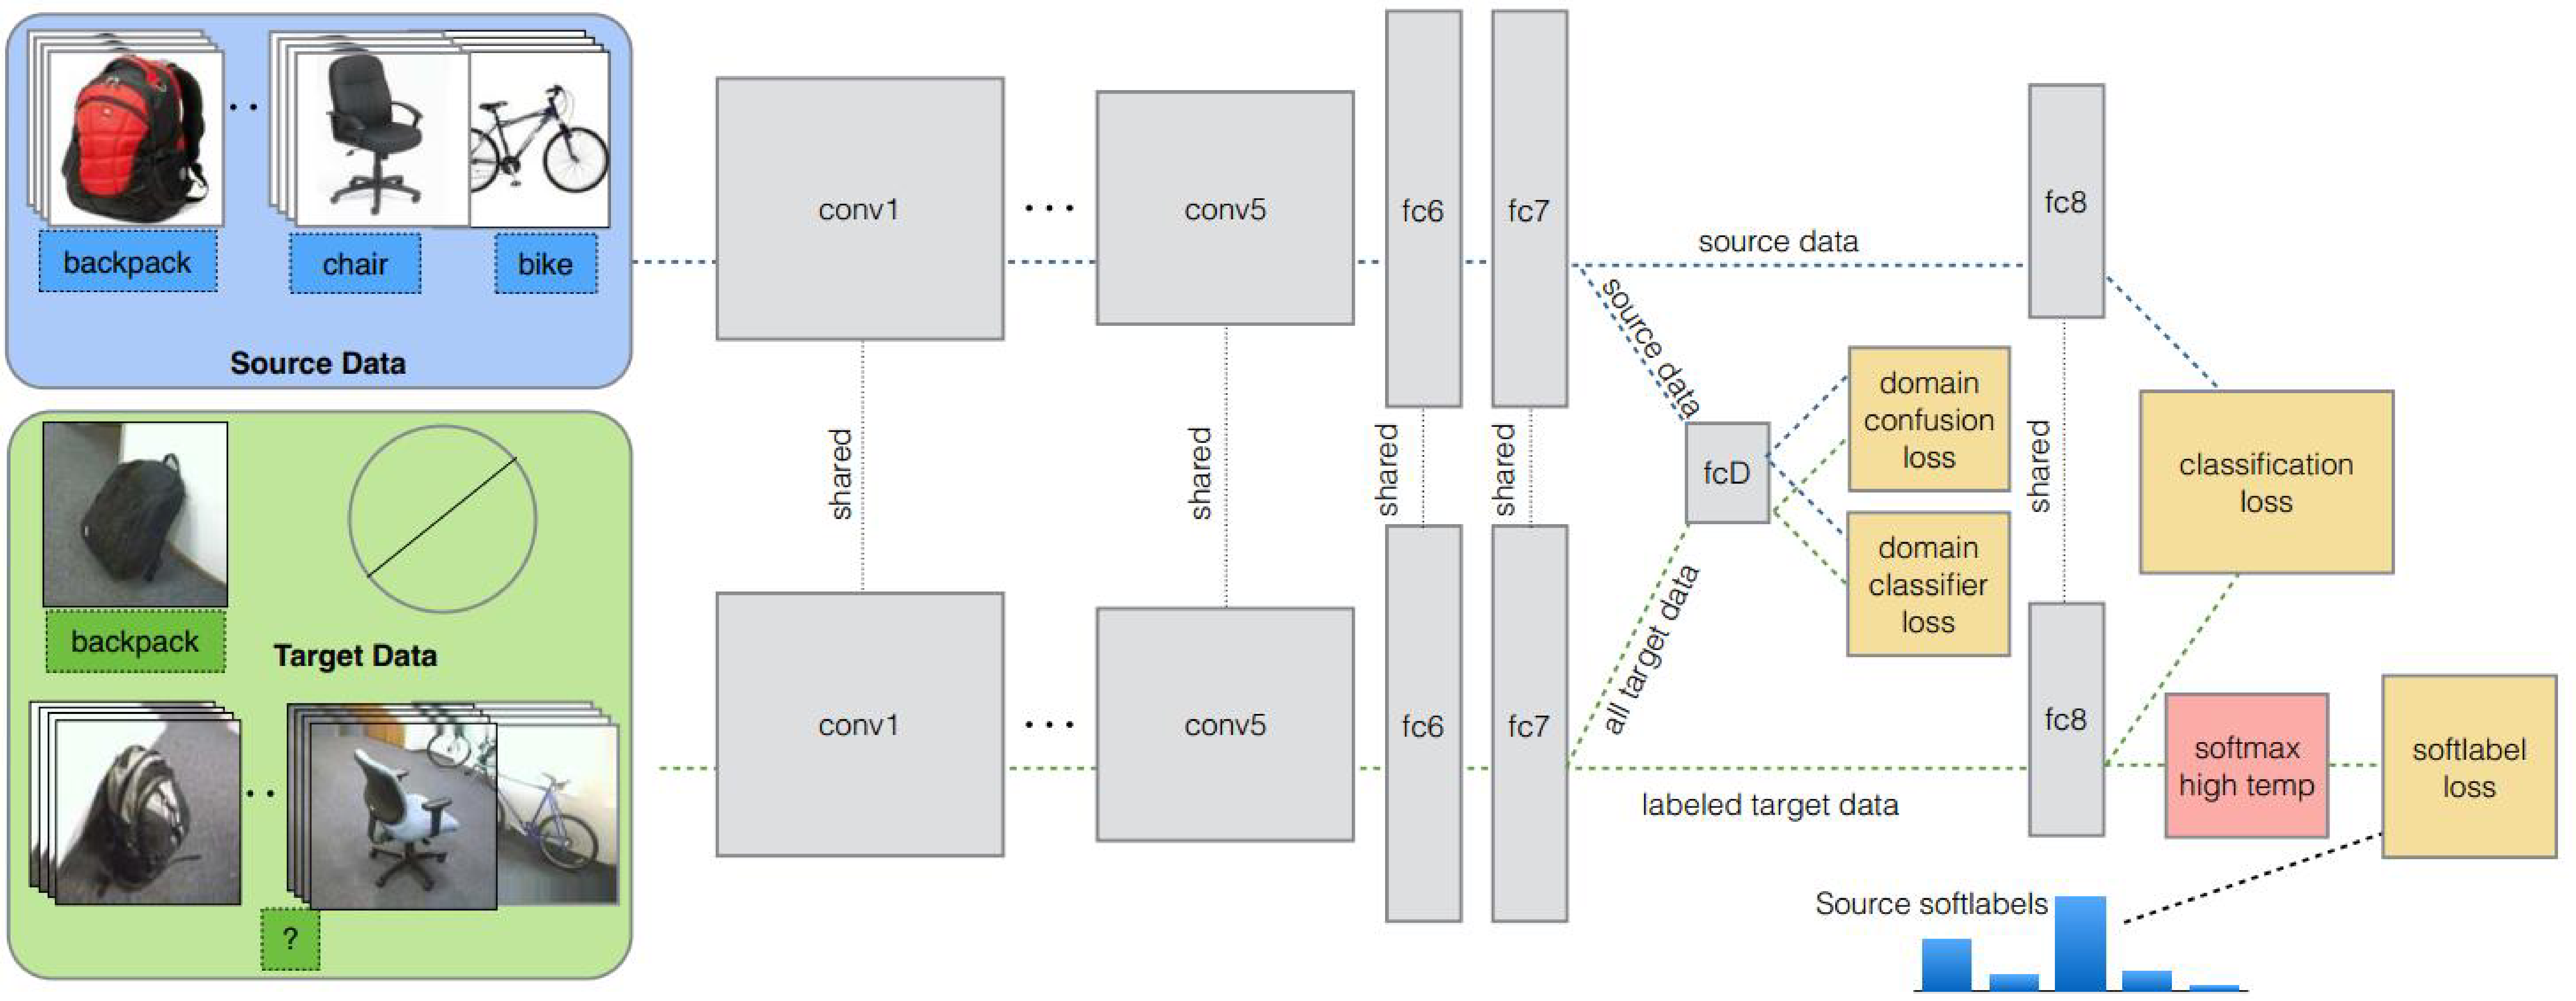
\includegraphics[scale=0.38]{./figures/fig-deep-tzeng2015.pdf}
	\caption{Joint CNN architecture for domain and task transfer方法示意图}
	\label{fig-deep-tzeng2015}
\end{figure}

Domain confusion就不用多说,和现有的一些比如DAN和JAN一样,直接对source和target的margina distribution进行估计即可。

什么是soft label loss?这和作者的motivation有关。不仅仅要适配两个domain的marginal distribution,也要把类别信息考虑进去。而target中有大量数据没有label,怎么办呢?可以利用source中的label信息。具体做法是:在网络对source进行训练的时候,把source的每一个样本处于每一个类的概率都记下来,然后,对于所有样本,属于每一个类的概率就可以通过求和再平均得到。如下图所示。这样的目的是:根据source中的类别分布关系,来对target做相应的约束。比如,source中和bike最相似的class,肯定是motorbike,而不是truck。这样有一定的道理。

但是在我看来,这就是深度网络版的conditional distribution adaptation。因为也对应于得到了每个类的proportion。只不过作者在这里取了个“soft label loss”这个好听的名字,再冠以“task transfer”这样高大上的名字。图~\ref{fig-deep-softlabel}是soft label的示意。

\begin{figure}[htbp]
	\centering
	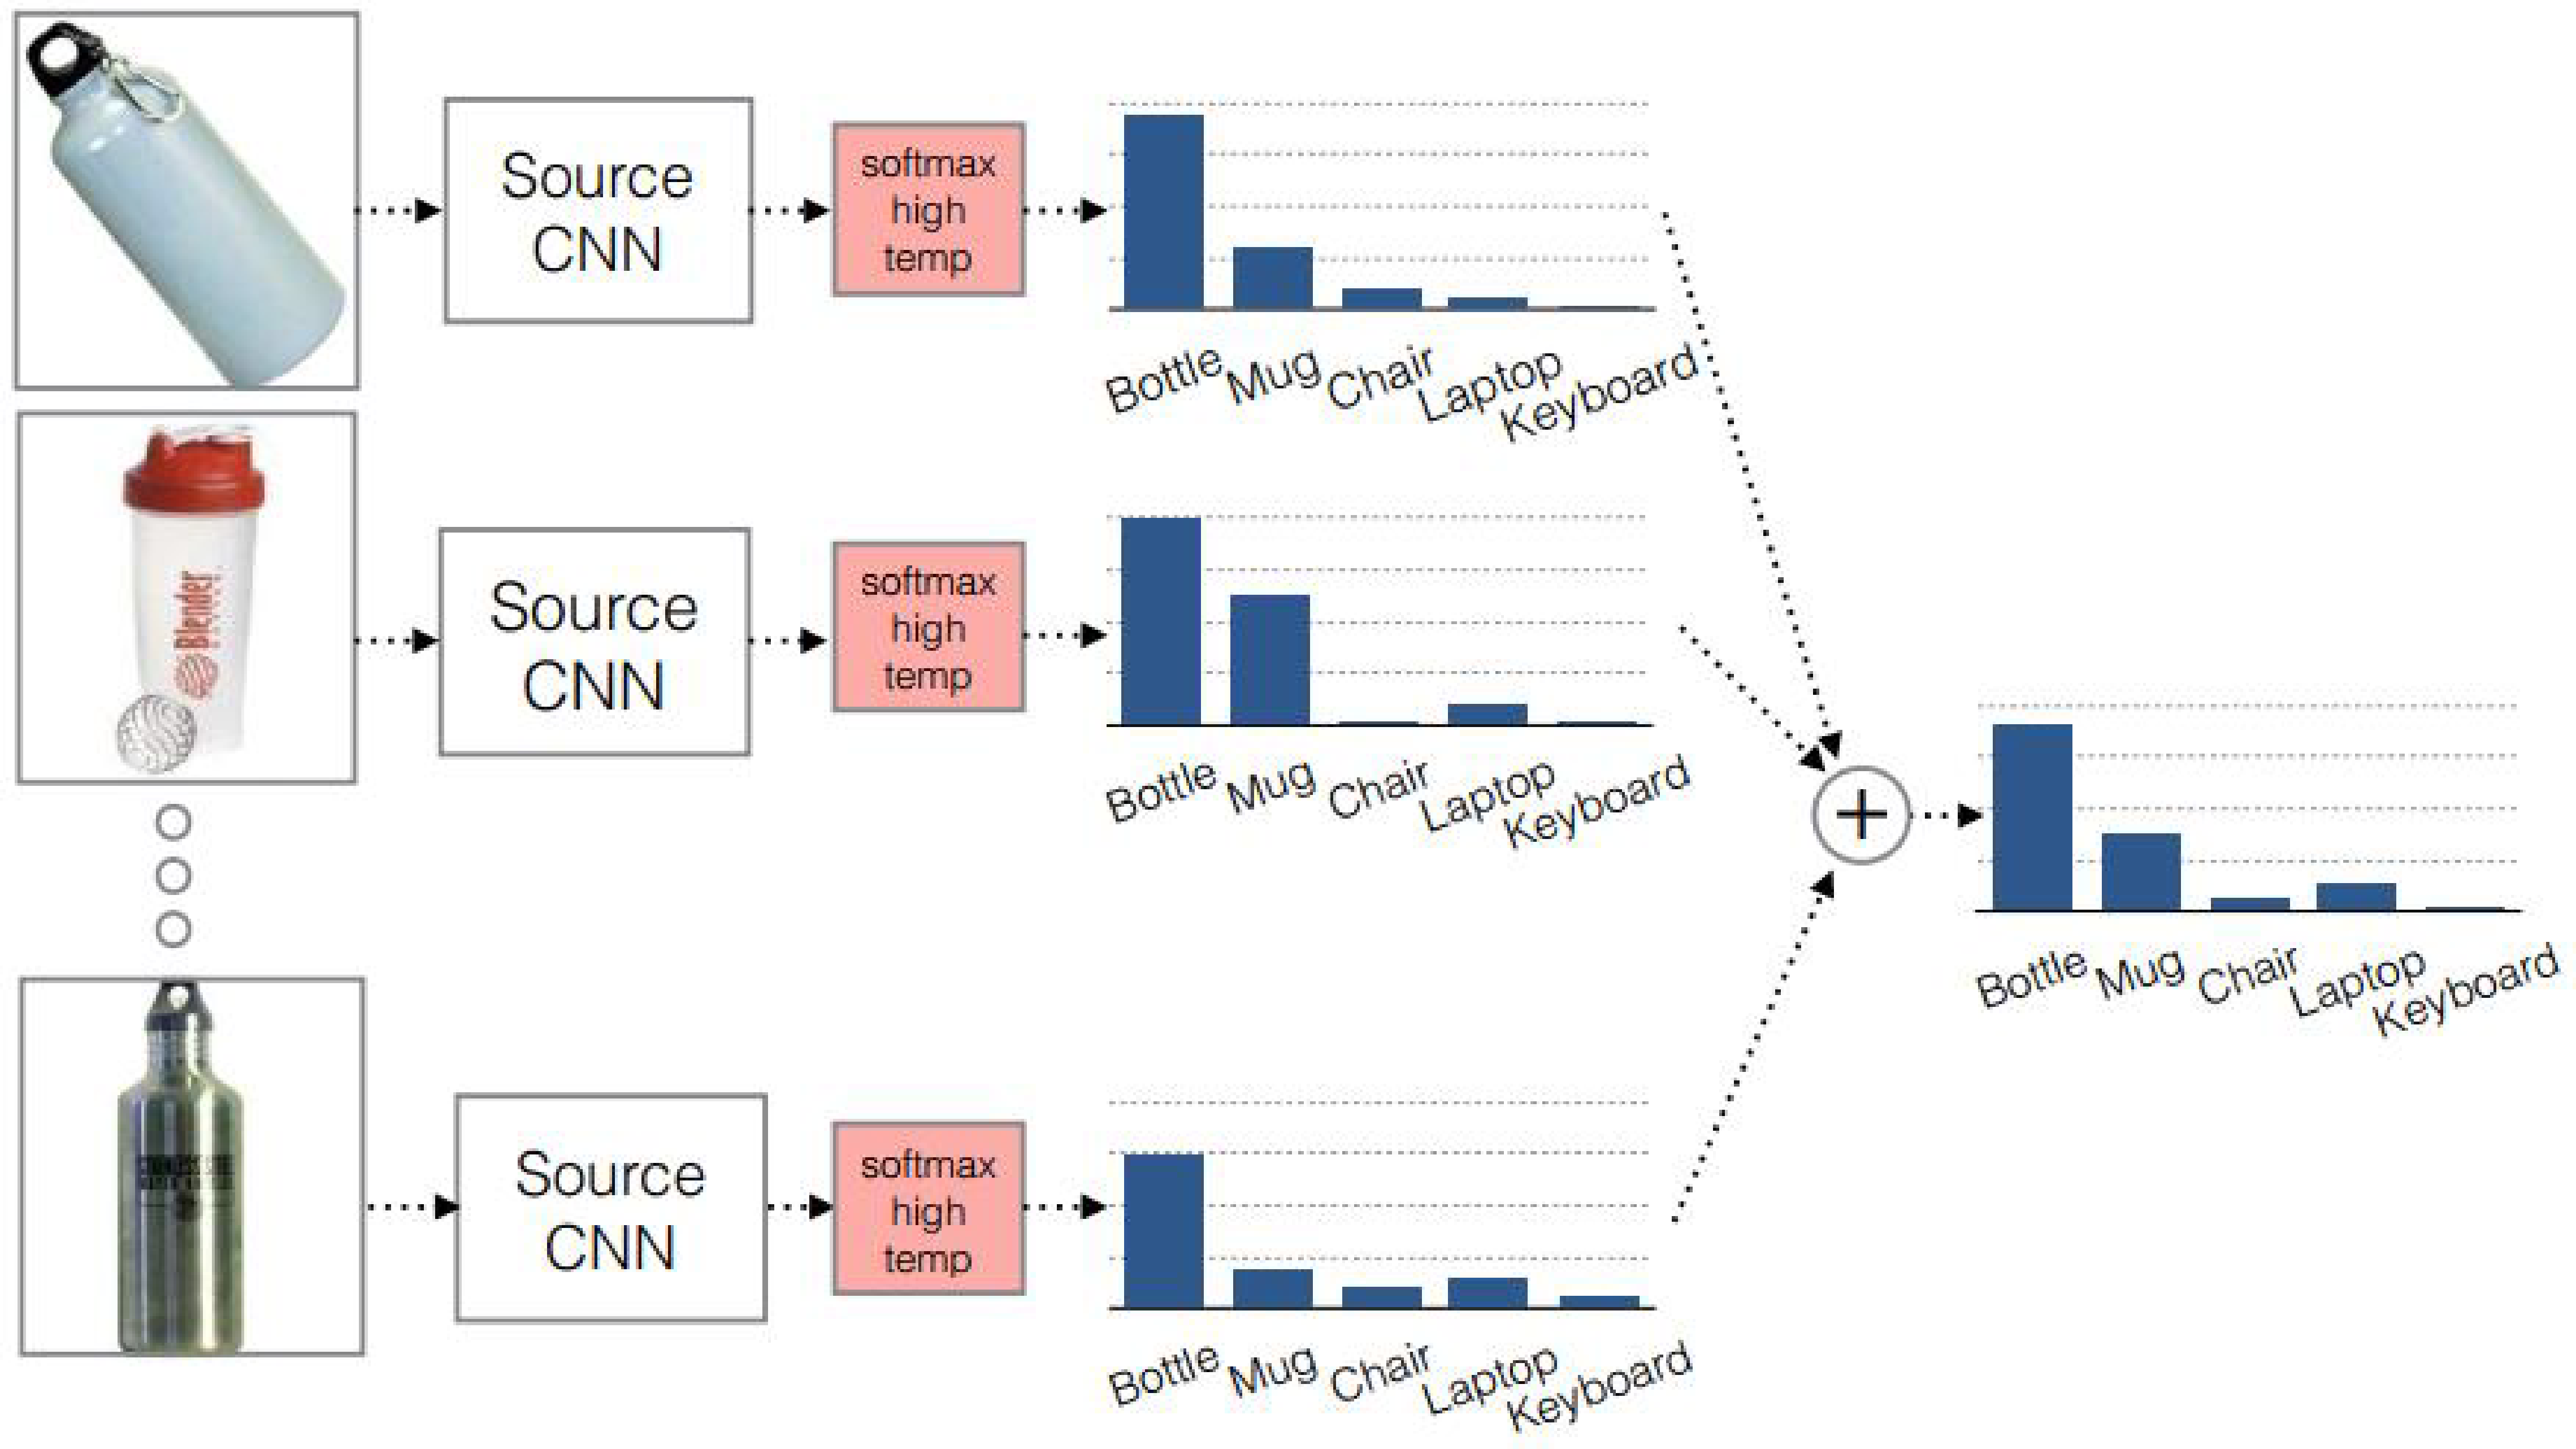
\includegraphics[scale=0.38]{./figures/fig-deep-softlabel.pdf}
	\caption{Softlabel示意图}
	\label{fig-deep-softlabel}
\end{figure}

\textbf{4. 深度联合分布自适应}

DAN的作者、清华大学的龙明盛在2017年机器学习顶级会议ICML上提出了JAN方法(Joint Adaptation Network)~\cite{long2017deep},在深度网络中同时进行联合分布的自适应和对抗学习。JAN方法将只对数据进行自适应的方式推广到了对类别的自适应,提出了JMMD度量(Joint MMD)。图~\ref{fig-deep-jan}是JAN的示意图。

\begin{figure}[htbp]
	\centering
	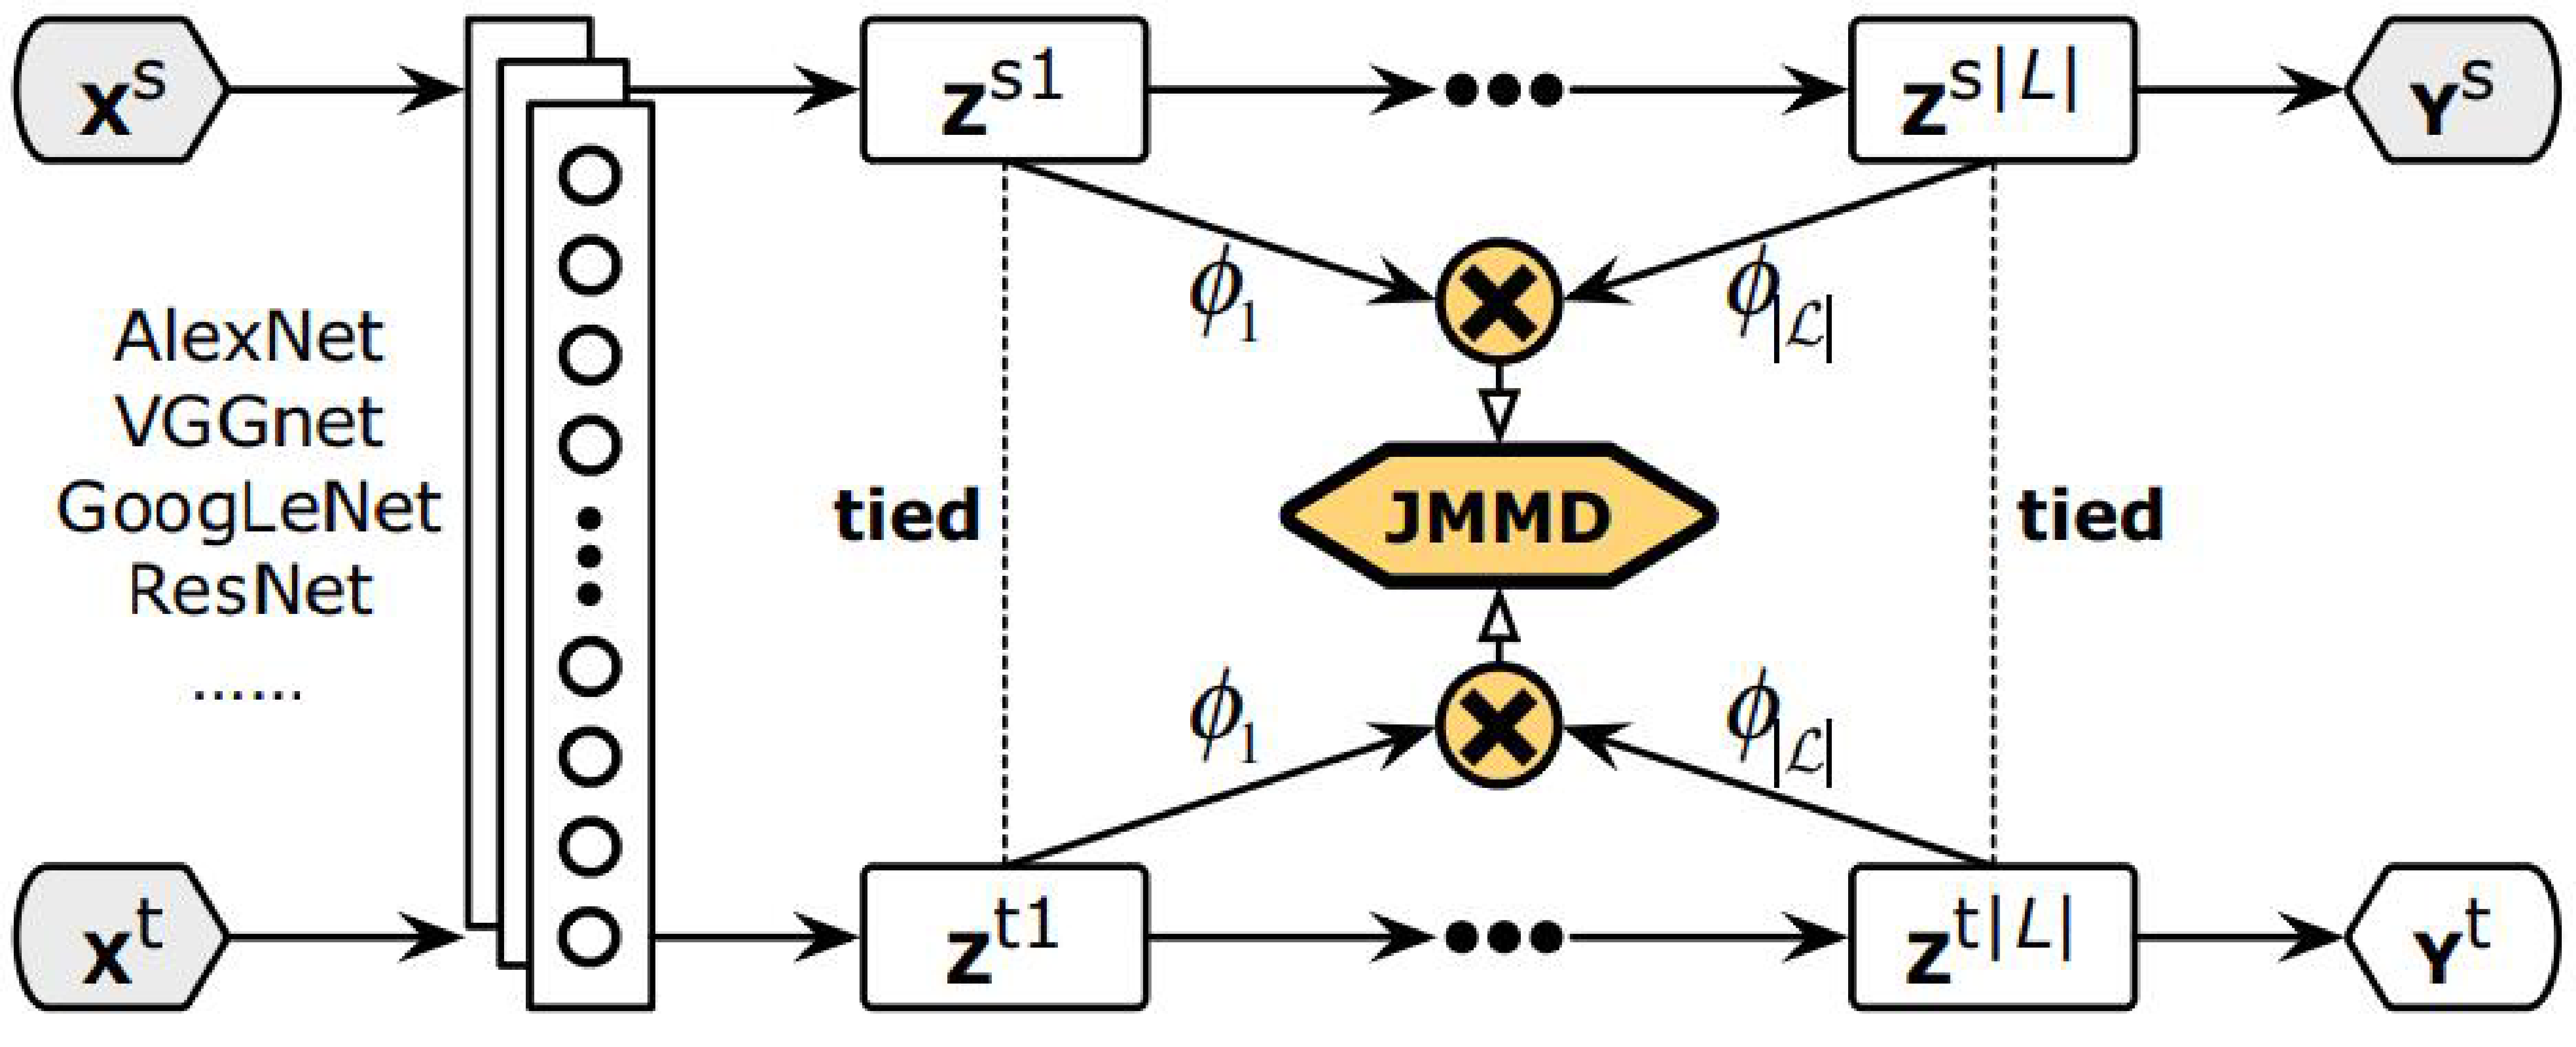
\includegraphics[scale=0.38]{./figures/fig-deep-jan.pdf}
	\caption{JAN方法示意图}
	\label{fig-deep-jan}
\end{figure}

\textbf{5. AdaBN}

与上述工作选择在已有网络层中增加适配层不同的是,北京大学的Haoyang Li和图森科技的Naiyan Wang等人提出了AdaBN(Adaptive Batch Normalization)~\cite{li2018adaptive},通过在归一化层加入统计特征的适配,从而完成迁移。

\begin{figure}[htbp]
	\centering
	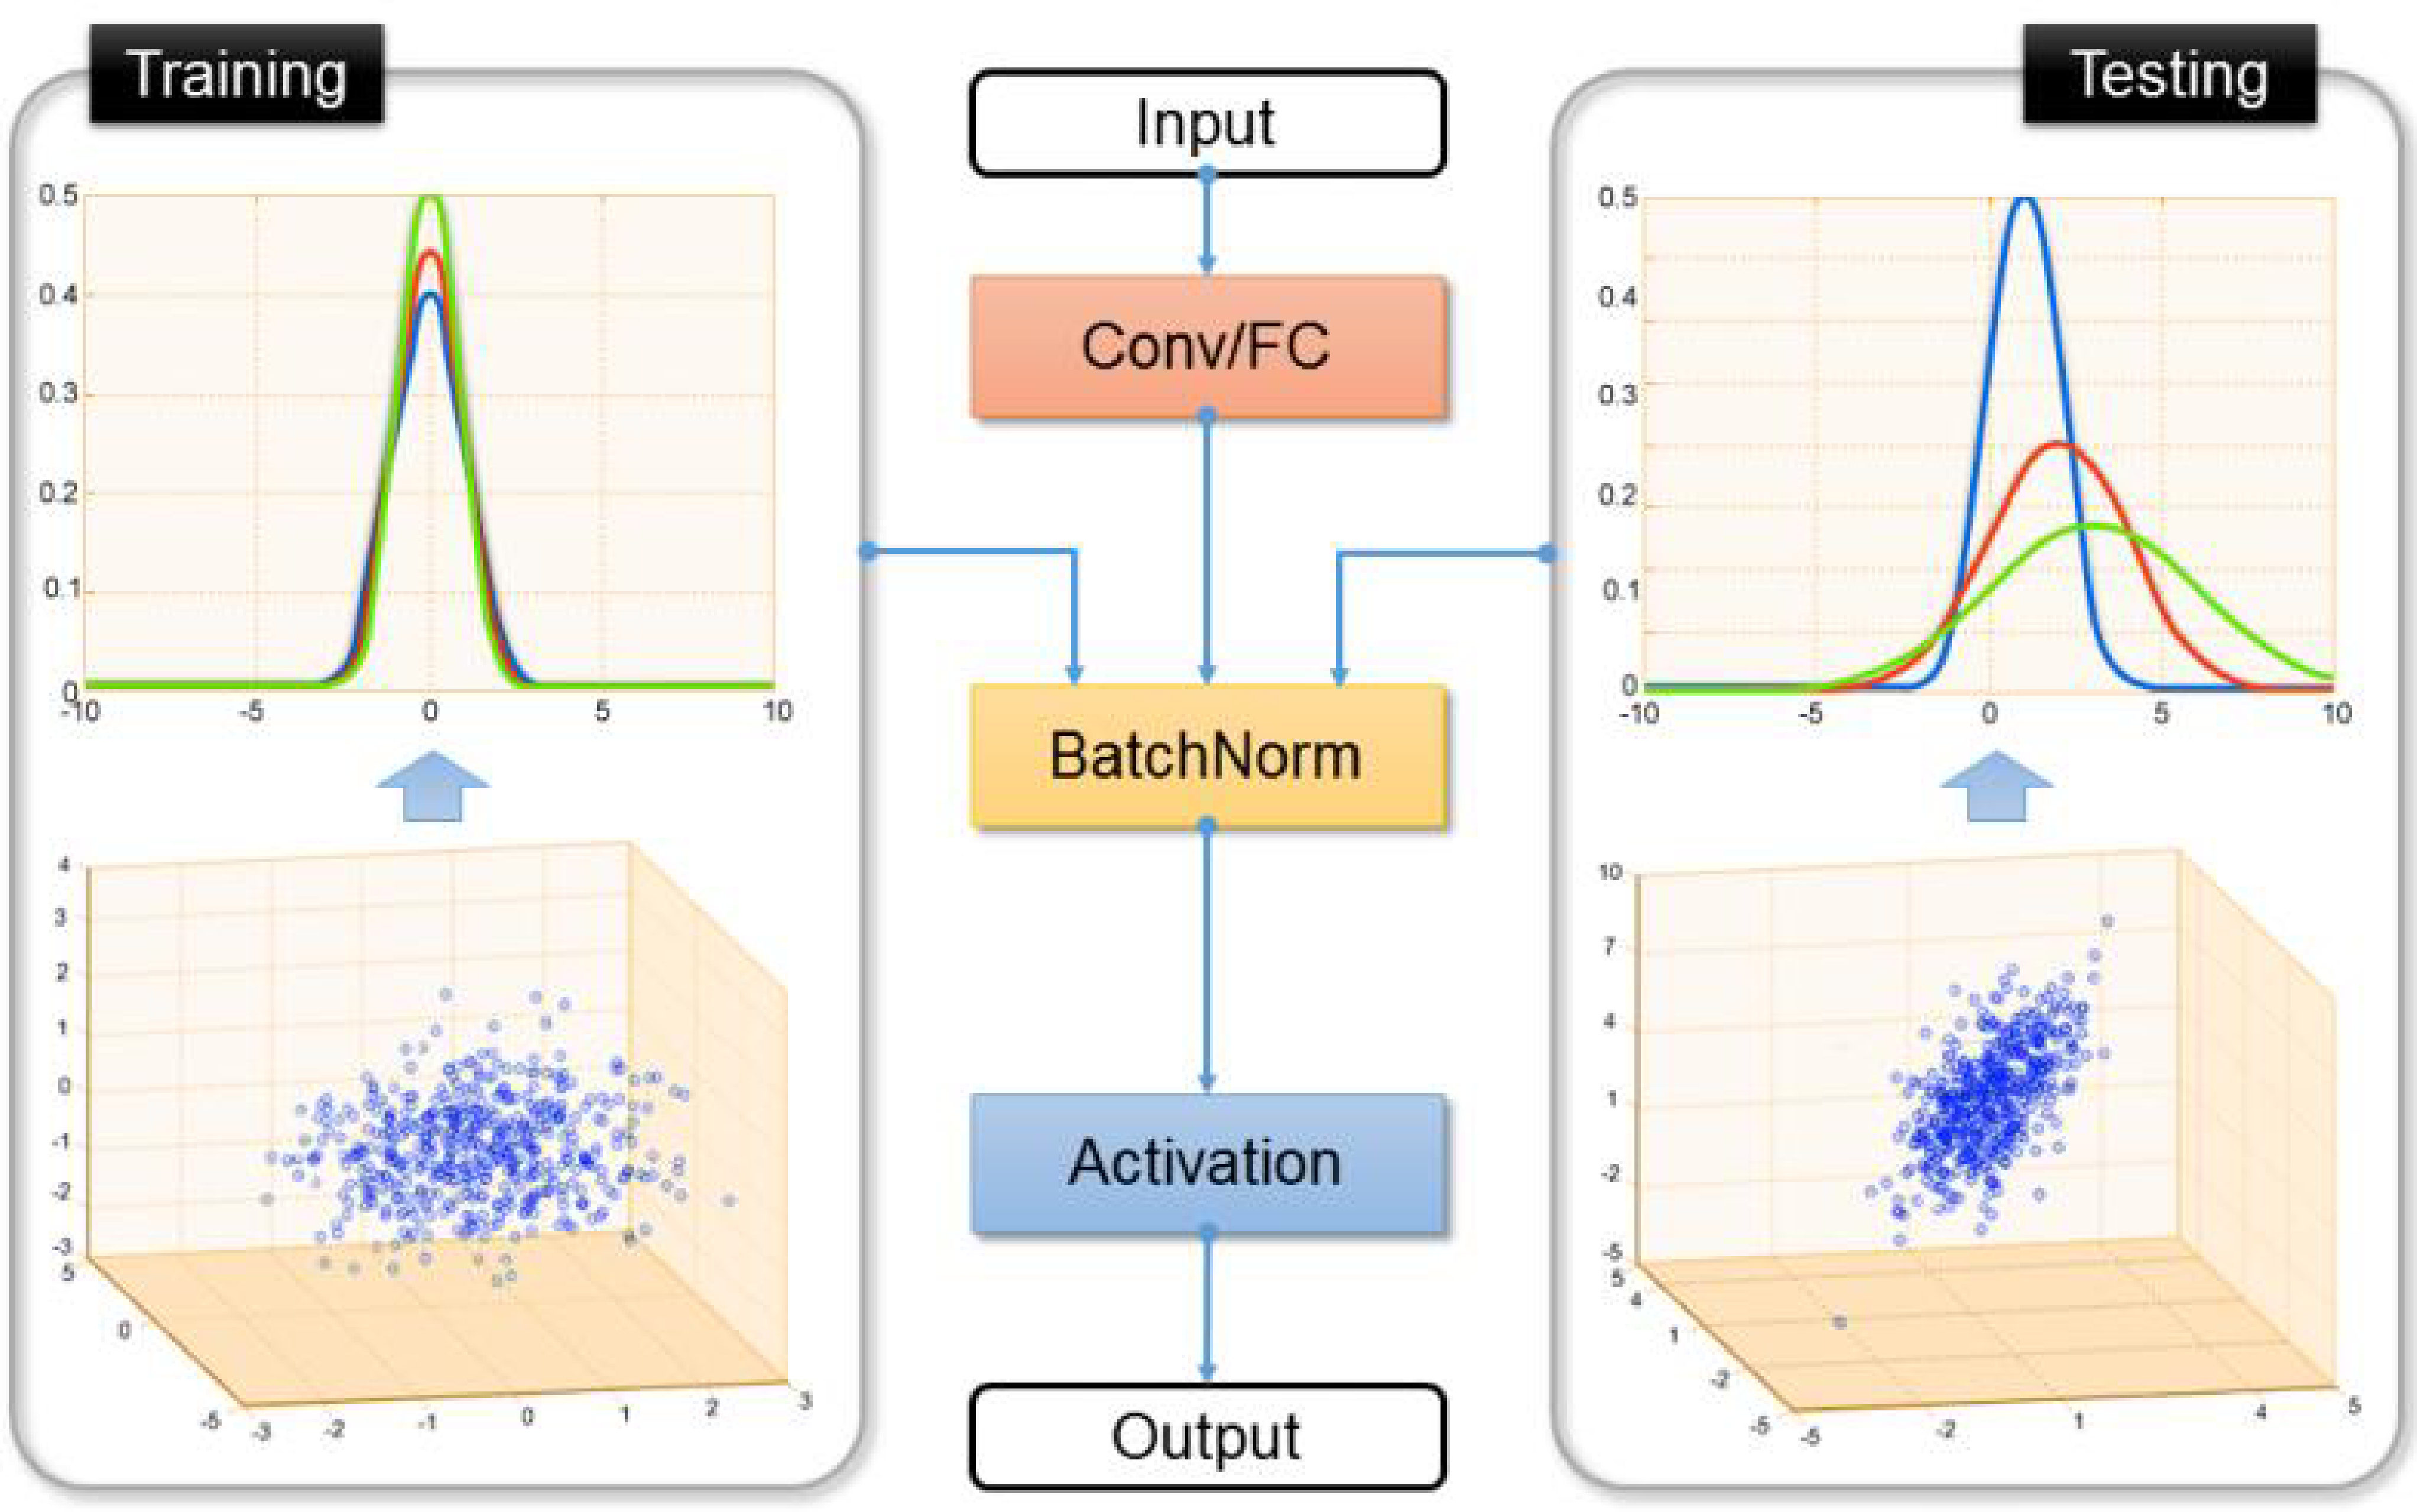
\includegraphics[scale=0.38]{./figures/fig-deep-adabn.pdf}
	\caption{AdaBN方法示意图}
	\label{fig-deep-adabn}
\end{figure}

AdaBN对比其他方法,实现相当简单。并且,方法本身不带有任何额外的参数。在许多公开数据集上都取得了很好的效果。

\subsubsection{小结}

基于深度网络进行迁移学习,其核心在于,找到网络需要进行自适应的层,并且对这些层加上自适应的损失度量。越来越多的研究者开始使用深度网络进行迁移学习~\cite{long2016deep,zhuo2017deep,zhuang2015supervised,sun2016deep,wei2016deep,luo2017label}。在这其中,几乎绝大多数方法都采用了卷积神经网络,在已训练好的模型(如AlexNet、Inception、GoogLeNet、Resnet等)上进行迁移。

特别地,最近意大利的学者Carlucci等人在2017年计算机视觉领域顶级会议ICCV上提出了自动深度网络自适应层(AutoDIAL, Automatic DomaIn Alignment Layers)~\cite{carlucci2017autodial}。该方法可以很简单地被加入现有的深度网络中,实现自动的自适应学习,使得深度网络的迁移更便捷。

由于篇幅和时间所限,我们未对所有新出现的研究工作给予介绍,仅在这里介绍了其中最具代表性的几种方法。但是绝大多数方法的原理都和我们已介绍过的大同小异。请读者持续关注最新发表的研究成果。

\subsection{深度对抗网络迁移}

生成对抗网络GAN(Generative Adversarial Nets)~\cite{goodfellow2014generative}是目前人工智能领域最炙手可热的概念之一。其也被深度学习领军人物Yann Lecun评为近年来最令人欣喜的成就。由此发展而来的对抗网络,也成为了提升网络性能的利器。本小节介绍深度对抗网络用于解决迁移学习问题方面的基本思路以及代表性研究成果。

\subsubsection{基本思路}

GAN受到自博弈论中的二人零和博弈(two-player game)思想的启发而提出。它一共包括两个部分:一部分为生成网络(Generative Network),此部分负责生成尽可能地以假乱真的样本,这部分被成为\textit{生成器}(Generator);另一部分为判别网络(Discriminative Network),此部分负责判断样本是真实的,还是由生成器生成的,这部分被成为\textit{判别器}(Discriminator)。生成器和判别器的互相博弈,就完成了对抗训练。

GAN的目标很明确:生成训练样本。这似乎与迁移学习的大目标有些许出入。然而,由于在迁移学习中,天然地存在一个源领域,一个目标领域,因此,我们可以免去生成样本的过程,而直接将其中一个领域的数据(通常是目标域)当作是生成的样本。此时,生成器的职能发生变化,不再生成新样本,而是扮演了特征提取的功能:不断学习领域数据的特征,使得判别器无法对两个领域进行分辨。这样,原来的生成器也可以称为特征提取器(Feature Extractor)。

通常用$G_f$来表示特征提取器,用$G_d$来表示判别器。

正是基于这样的领域对抗的思想,深度对抗网络可以被很好地运用于迁移学习问题中。

与深度网络自适应迁移方法类似,深度对抗网络的损失也由两部分构成:网络训练的损失$\ell_c$和领域判别损失$\ell_d$:

\begin{equation}
	\ell = \ell_c(\mathcal{D}_s,\mathbf{y}_s) + \lambda \ell_d(\mathcal{D}_s,\mathcal{D}_t)
\end{equation}

\subsubsection{核心方法}

\textbf{1. DANN}

Yaroslav Ganin等人~\cite{ganin2016domain}首先在神经网络的训练中加入了对抗机制,作者将他们的网络称之为DANN(Domain-Adversarial Neural Network)。在此研究中,网络的学习目标是:\textit{生成的特征尽可能帮助区分两个领域的特征,同时使得判别器无法对两个领域的差异进行判别}。该方法的领域对抗损失函数表示为:

\begin{equation}
	\ell_d = \max \left[-\frac{1}{n} \sum_{i=1}^{n} \mathcal{L}^i_d(\mathbf{W},\mathbf{b},\mathbf{u},z) - \frac{1}{n'} \sum_{i=n+1}^{N} \mathcal{L}^i_d(\mathbf{W},\mathbf{b},\mathbf{u},z)\right]
\end{equation}

其中的$\mathcal{L}_d$表示为

\begin{equation}
	\mathcal{L}_d(G_d(G_f(\mathbf{x}_i)),d_i) = d_i \log \frac{1}{G_d(G_f(\mathbf{x}_i))} + (1 - d_i) \log \frac{1}{G_d(G_f(\mathbf{x}_i))}
\end{equation}

\textbf{2. DSN}

来自Google Brain的Bousmalis等人通过提出DSN网络(Domain Separation Networks)~\cite{bousmalis2016domain}对DANN进行了扩展。DSN认为,源域和目标域都由两部分构成:公共部分和私有部分。公共部分可以学习公共的特征,私有部分用来保持各个领域独立的特性。DSN进一步对损失函数进行了定义:

\begin{equation}
	\ell = \ell_{task} + \alpha \ell_{recon} + \beta \ell_{difference} + \gamma \ell_{similarity}
\end{equation}

除去网络的常规训练损失$\ell_{task}$外,其他损失的含义如下:
\begin{itemize}
	\item $\ell_{recon}$: 重构损失,确保私有部分仍然对学习目标有作用
	\item $\ell_{difference}$: 公共部分与私有部分的差异损失
	\item $\ell_{similarity}$: 源域和目标域公共部分的相似性损失
\end{itemize}

图~\ref{fig-deep-dsn}是DSN方法的示意图。

\begin{figure}[htbp]
	\centering
	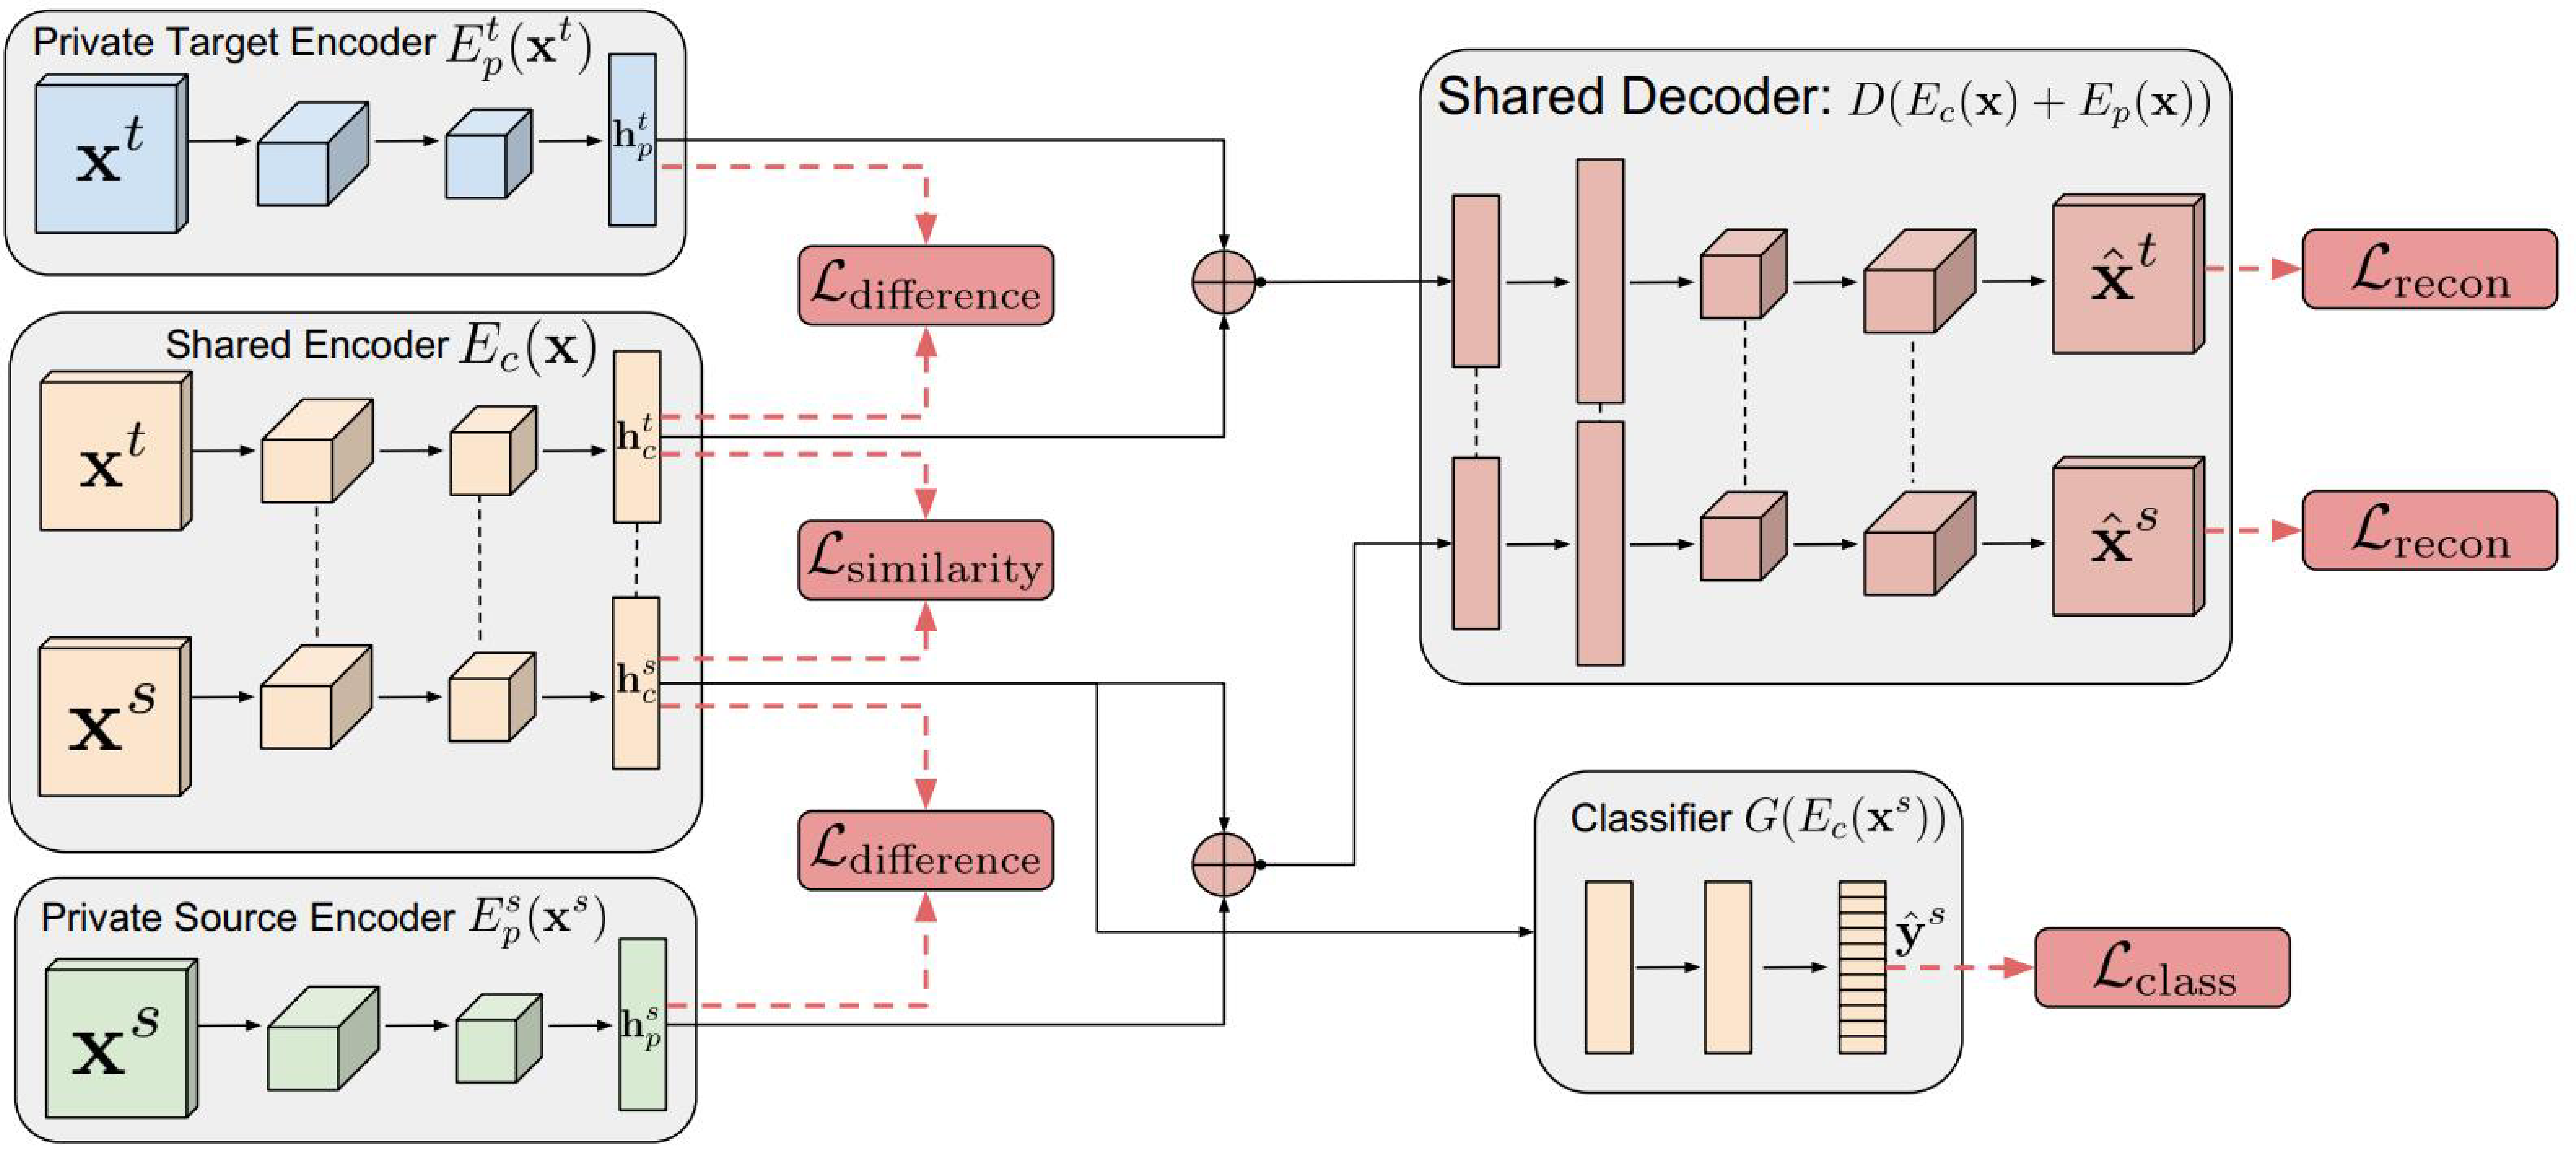
\includegraphics[scale=0.32]{./figures/fig-deep-dsn.pdf}
	\caption{DSN方法示意图}
	\label{fig-deep-dsn}
\end{figure}

DDC方法的作者、加州大学伯克利分校的Tzeng等人在2017年发表于计算机视觉顶级会议CVPR上的文章提出了ADDA方法(Adversarial Discriminative Domain Adaptation)~\cite{tzeng2017adversarial}。ADDA是一个通用的框架,现有的很多方法都可被看作是ADDA的特例。上海交通大学的研究者们用Wasserstein GAN进行迁移学习~\cite{shen2018w},Liu等人提出了Coupled GAN用于迁移学习~\cite{liu2016coupled}。这些工作都大体上按照之前思路进行。

\textbf{3. SAN}

清华大学龙明盛团队2018年发表在计算机视觉顶级会议CVPR上的文章提出了一个选择性迁移网络(Partial Transfer Learning)。作者认为,在大数据时代,通常我们会有大量的源域数据。这些源域数据比目标域数据,在类别上通常都是丰富的。比如基于ImageNet训练的图像分类器,必然是针对几千个类别进行的分类。我们实际用的时候,目标域往往只是其中的一部分类别。这样就会带来一个问题:那些只存在于源域中的类别在迁移时,会对迁移结果产生负迁移影响。

这种情况通常来说是非常普遍的。因此,就要求相应的迁移学习方法能够对目标域,选择相似的源域样本(类别),同时也要避免负迁移。但是目标域通常是没有标签的,不知道和源域中哪个类别更相似。作者指出这个问题叫做partial transfer learning。这个partial,就是只迁移源域中那部分和目标域相关的样本。图~\ref{fig-deep-partial}展示了部分迁移学习的思想。

\begin{figure}[htbp]
	\centering
	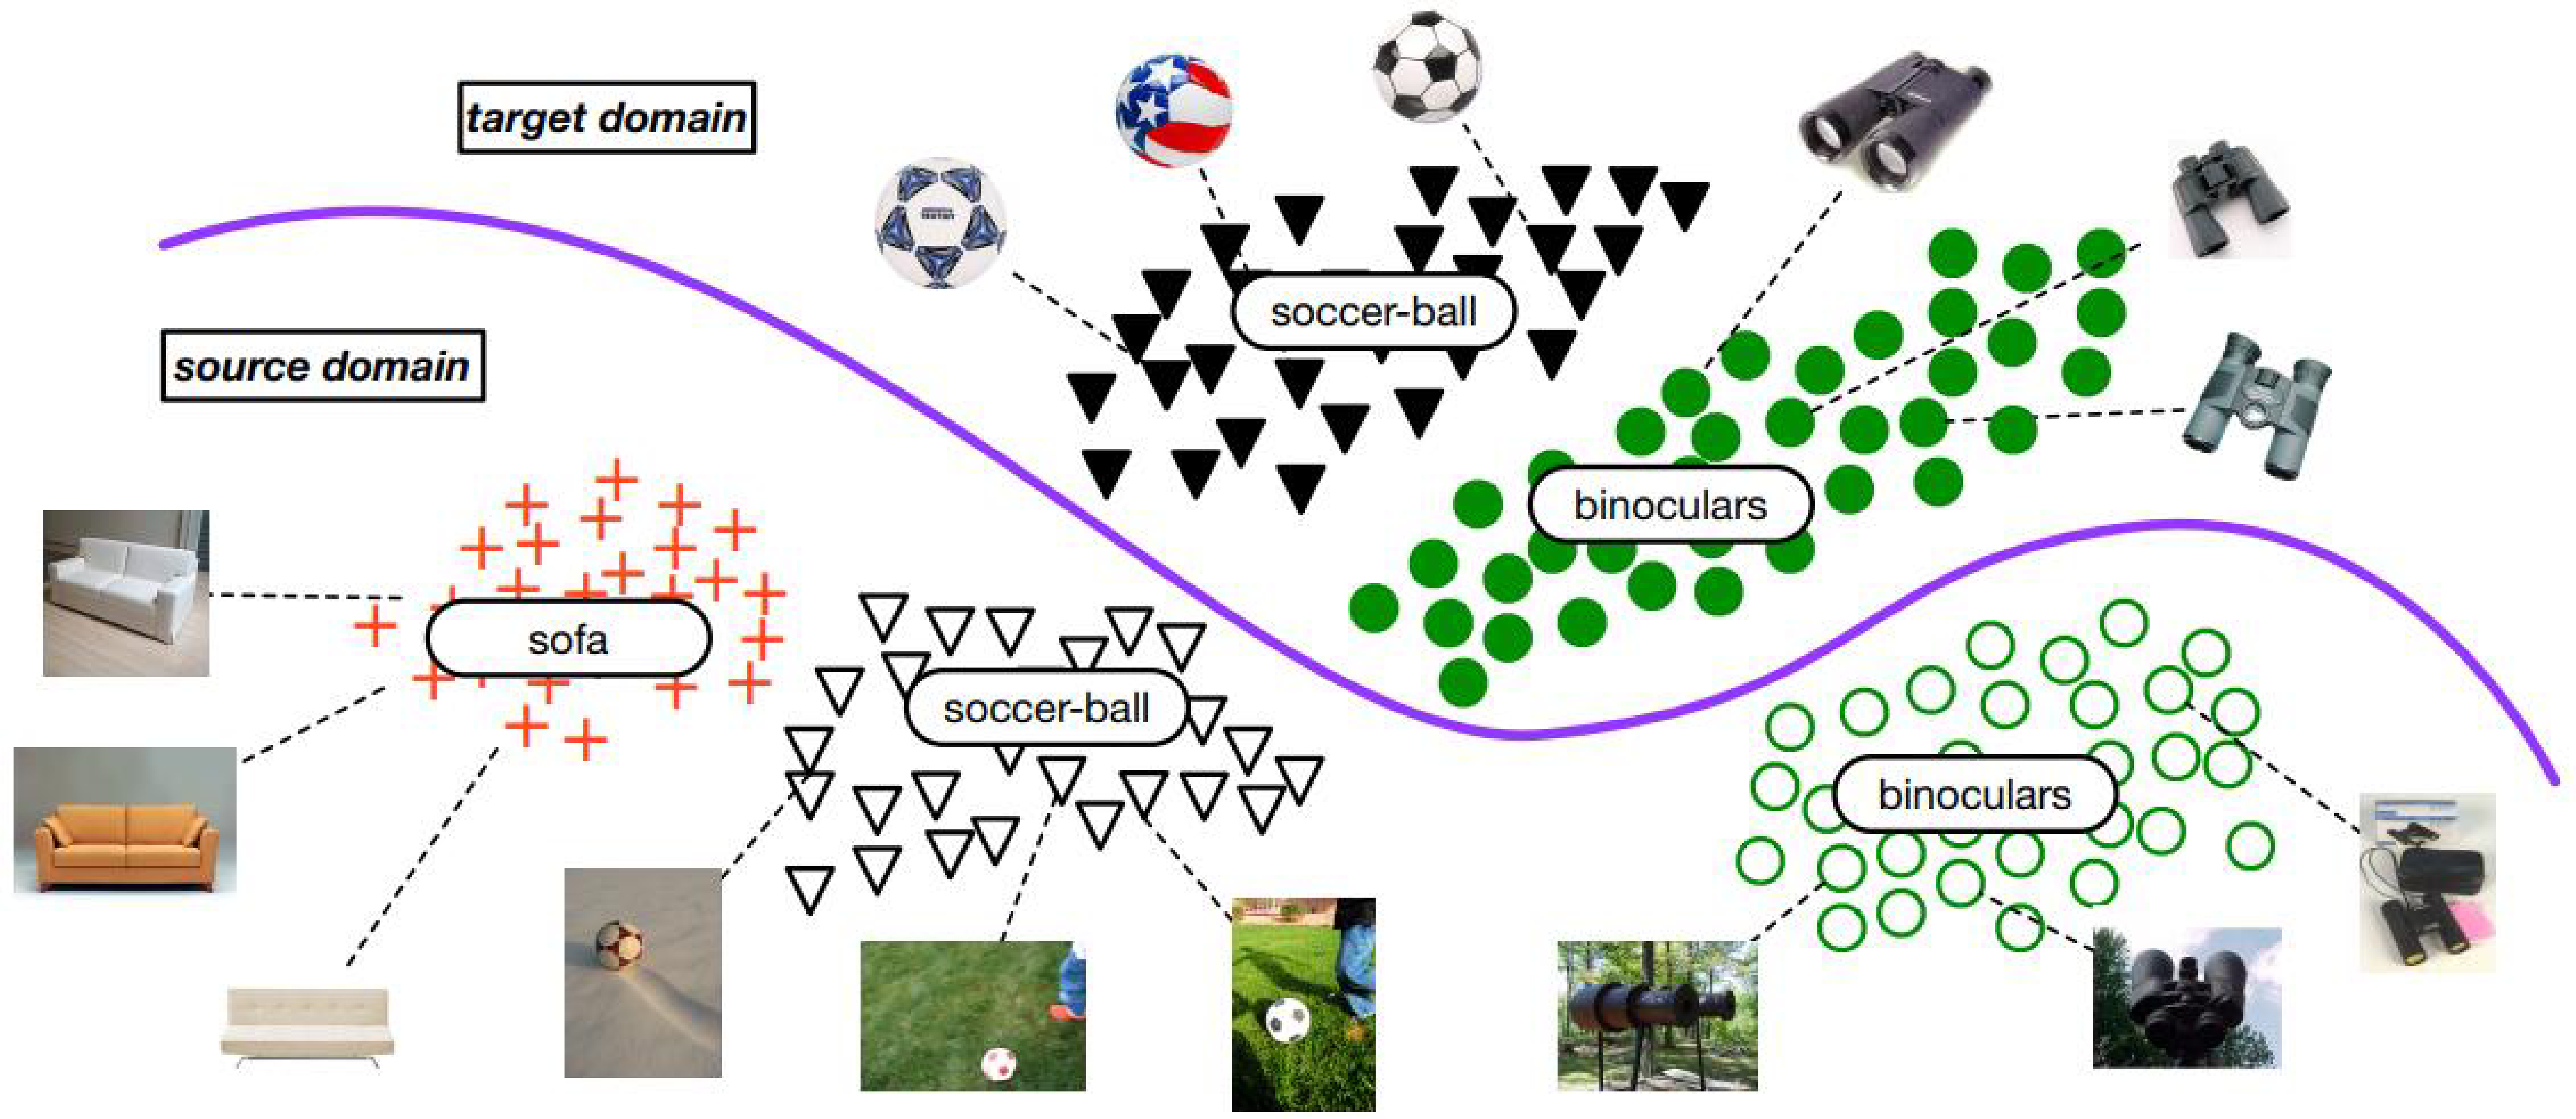
\includegraphics[scale=0.32]{./figures/fig-deep-partial.pdf}
	\caption{部分迁移学习示意图}
	\label{fig-deep-partial}
\end{figure}

作者提出了一个叫做Selective Adversarial Networks (SAN)~\cite{cao2017partial}的方法来处理partial transfer问题。在partial问题中,传统的对抗网络不再适用。所以就需要对进行一些修改,使得它能够适用于partial问题。

因为不知道目标域的标签,也就没办法知道到底是源域中哪些类是目标域的。为了达到这个目的,作者对目标域按照类别分组,把原来的一整个判别器分成了$|\mathcal{C}_s|$个:$G^k_d$,每一个子判别器都对它所在的第$k$个类进行判别。作者观察到了这样的事实:对于每个数据点$\mathbf{x}_i$来说,分类器的预测结果 $\hat{\mathbf{y}}_i$ 其实是对于整个类别空间的一个\textit{概率分布}。因此,在进行对抗时,需要考虑每个样本属于每个类别的影响。这个影响就是由概率来刻画。所以作者提出了一个概率权重的判别器:

\begin{equation}
	L'_d=\frac{1}{n_s+n_t} \sum_{k=1}^{|\mathcal{C}_s|} \sum_{\mathbf{x}_i \in \mathcal{D}_s + \mathcal{D}_t}^{} \hat{y}^k_i L^k_d(G^k_d(G_f(\mathbf{x}_i)),d_i)
\end{equation}

上面这个式子能很好地在partial transfer情景下,避免负迁移。这种约束是样本级别的,就是可以控制尽可能让更相似的样本参与迁移。除此之外,作者还介绍了一个类别级别的约束,可以很好地避免不在目标域中的那些类别不参与迁移。于是,进一步地,变成了下面的约束

\begin{equation}
	L'_d=\frac{1}{n_s+n_t} \sum_{k=1}^{|\mathcal{C}_s|} \sum_{\mathbf{x}_i \in \mathcal{D}_s + \mathcal{D}_t}^{} (\frac{1}{n_t} \sum_{\mathbf{x}_i^{} \in \mathcal{D}_t}\hat{y}^k_i) L^k_d(G^k_d(G_f(\mathbf{x}_i)),d_i)
\end{equation}

上面这个式子比较依赖于之前说的每个样本的预测概率。为了消除这个影响,作者又在目标域上加了一项熵最小化

\begin{equation}
	E=\frac{1}{n_t} \sum_{\mathbf{x}_i \in \mathcal{D}_t} H(G_y(G_f(\mathbf{x}_i)))
\end{equation}

\textbf{4. DAAN}

最近,Yu等人在~\cite{yu2019transfer}中将动态分布适配的概念进一步扩展到了对抗网络中,证明了对抗网络中同样存在边缘分布和条件分布不匹配的问题。作者提出一个动态对抗适配网络DAAN (Dynamic Adversarial Adaptation Networks)来解决对抗网络中的动态分布适配问题,取得了当前的最好效果。图~\ref{fig-deep-daan}展示了DAAN的架构。

\begin{figure}[htbp]
	\centering
	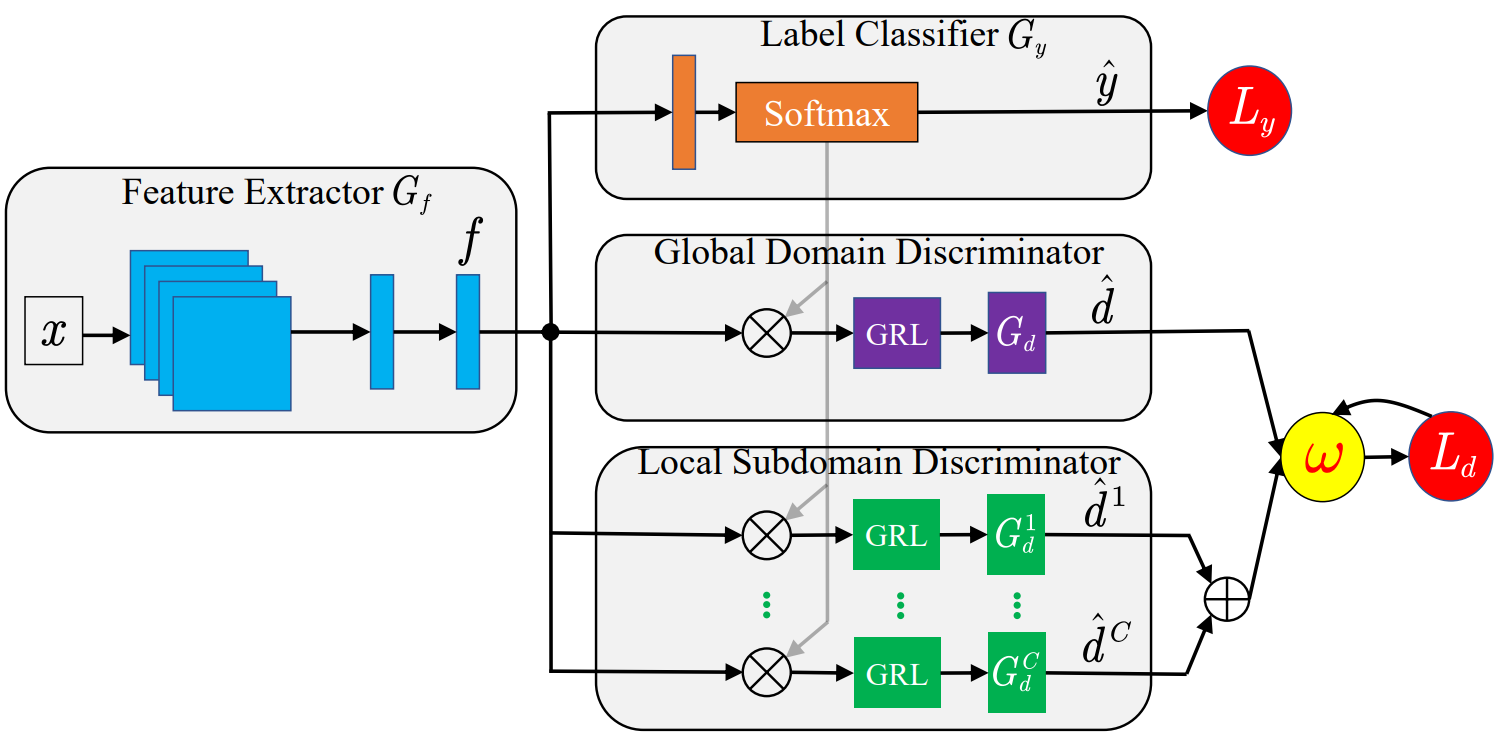
\includegraphics[scale=.35]{./figures/fig-distribution-daan.png}
	\caption{动态对抗适配网络DAAN结构示意图}
	\label{fig-deep-daan}
\end{figure}

\subsubsection{小结}

使用对抗网络进行迁移学习是近年来的研究热点。我们期待在这个领域会有越来越多的工作发表。
\newpage

\definecolor{dkgreen}{rgb}{0,0.6,0}
\definecolor{gray}{rgb}{0.5,0.5,0.5}
\definecolor{mauve}{rgb}{0.58,0,0.82}

\lstset{ %
	language=Matlab,                % the language of the code
	basicstyle=\footnotesize,           % the size of the fonts that are used for the code
	numbers=left,                   % where to put the line-numbers
	numberstyle=\tiny\color{gray},  % the style that is used for the line-numbers
	stepnumber=2,                   % the step between two line-numbers. If it's 1, each line 
	% will be numbered
	numbersep=5pt,                  % how far the line-numbers are from the code
	backgroundcolor=\color{white},      % choose the background color. You must add \usepackage{color}
	showspaces=false,               % show spaces adding particular underscores
	showstringspaces=false,         % underline spaces within strings
	showtabs=false,                 % show tabs within strings adding particular underscores
	frame=single,                   % adds a frame around the code
	rulecolor=\color{black},        % if not set, the frame-color may be changed on line-breaks within not-black text (e.g. commens (green here))
	tabsize=2,                      % sets default tabsize to 2 spaces
	captionpos=b,                   % sets the caption-position to bottom
	breaklines=true,                % sets automatic line breaking
	breakatwhitespace=false,        % sets if automatic breaks should only happen at whitespace
	title=\lstname,                   % show the filename of files included with \lstinputlisting;
	% also try caption instead of title
	keywordstyle=\color{blue},          % keyword style
	commentstyle=\color{dkgreen},       % comment style
	stringstyle=\color{mauve},         % string literal style
	escapeinside={\%*}{*)},            % if you want to add LaTeX within your code
	morekeywords={*,...}               % if you want to add more keywords to the set
}

\section{上手实践}

以上对迁移学习基本方法的介绍还只是停留在算法的阶段。对于初学者来说,不仅需要掌握基础的算法知识,更重要的是,需要在实验中发现问题。本章的目的是为初学者提供一个迁移学习上手实践的介绍。通过一步步编写代码、下载数据,完成迁移学习任务。在本部分,我们以迁移学习中最为流行的图像分类为实验对象,在流行的Office+Caltech10数据集上完成。

迁移学习方法主要包括:传统的非深度迁移、深度网络的finetune、深度网络自适应、以及深度对抗网络的迁移。教程的目的是抛砖引玉,帮助初学者快速入门。由于网络上已有成型的深度网络的finetune、深度网络自适应、以及深度对抗网络的迁移教程,因此我们不再叙述这些方法,只在这里介绍非深度方法的教程。其他三种方法的地址分别是:

\begin{itemize}
	\item 深度网络的finetune:\href{https://github.com/jindongwang/transferlearning/tree/master/code/deep/finetune_AlexNet_ResNet}{用Pytorch对Alexnet和Resnet进行微调}、\href{https://pytorch.org/tutorials/beginner/transfer_learning_tutorial.html}{使用PyTorch进行finetune}
	\item 深度网络的自适应:\href{https://github.com/jindongwang/transferlearning/tree/master/code/deep/DDC_DeepCoral}{DDC/DCORAL方法的Pytorch代码}
	\item 深度对抗网络迁移:\href{https://github.com/jindongwang/transferlearning/tree/master/code/deep/DANN(RevGrad)}{DANN方法}
\end{itemize}

更多深度迁移方法的代码,请见\url{https://github.com/jindongwang/transferlearning/tree/master/code/deep}。

%\subsection{非深度迁移}

在众多的非深度迁移学习方法中,我们选择最经典的迁移方法之一、发表于IEEE TNN 2011的TCA(Transfer Component Analysis)~\cite{pan2011domain}方法进行实践。为了便于学习,我们同时用Matlab和Python实现了此代码。代码的链接为\url{https://github.com/jindongwang/transferlearning/tree/master/code/traditional/TCA}。下面我们对代码进行简单讲解。

\subsection{TCA方法代码实现}

\subsubsection{Matlab}

\textbf{1. 数据获取}

由于我们要测试非深度方法,因此,选择SURF特征文件作为算法的输入。SURF特征文件可以从网络上~\footnote{\url{https://pan.baidu.com/s/1bp4g7Av}}下载。下载到的文件主要包含4个.mat文件:Caltech.mat, amazon.mat, webcam.mat, dslr.mat。它们恰巧对应4个不同的领域。彼此之间两两一组,就是一个迁移学习任务。每个数据文件包含两个部分:fts为800维的特征,labels为对应的标注。在测试中,我们选择由Caltech.mat作为源域,由amazon.mat作为目标域。Office+Caltech10数据集的介绍可以在本手册的第~\ref{sec-dataset}部分找到。

我们对数据进行加载并做简单的归一化,将最后的数据存入$X_s,Y_s,X_t,Y_t$这四个变量中。这四个变量分别对应源域的特征和标注、以及目标域的特征和标注。代码如下:

\begin{lstlisting}[title=Matlab加载数据, frame=shadowbox]
load('Caltech.mat');     % source domain
fts = fts ./ repmat(sum(fts,2),1,size(fts,2)); 
Xs = zscore(fts,1);    clear fts
Ys = labels;           clear labels

load('amazon.mat');    % target domain
fts = fts ./ repmat(sum(fts,2),1,size(fts,2)); 
Xt = zscore(fts,1);     clear fts
Yt = labels;            clear labels
\end{lstlisting}

\textbf{2. 算法精炼}

TCA主要进行边缘分布自适应。通过整理化简,TCA最终的求解目标是:
\begin{equation}
\label{equ-eigen}
\begin{split}
\left(\mathbf{X} \mathbf{M} \mathbf{X}^\top + \lambda \mathbf{I}\right) \mathbf{A} =\mathbf{X} \mathbf{H} \mathbf{X}^\top \mathbf{A} \Phi 
\end{split}
\end{equation}

上述表达式可以通过Matlab自带的$\mathrm{eigs()}$函数直接求解。$\mathbf{A}$就是我们要求解的变换矩阵。下面我们需要明确各个变量所指代的含义:

\begin{itemize}
	\item $\mathbf{X}$: 由源域和目标域数据共同构成的数据矩阵
	\item $C$: 总的类别个数。在我们的数据集中,$C=10$
	\item $\mathbf{M}_c$: MMD矩阵。当$c=0$时为全MMD矩阵;当$c>1$时对应为每个类别的矩阵。
	\item $\mathbf{I}$:单位矩阵
	\item $\lambda$:平衡参数,直接给出
	\item $\mathbf{H}$: 中心矩阵,直接计算得出
	\item $\Phi$: 拉格朗日因子,不用理会,求解用不到
\end{itemize}

\textbf{3. 编写代码}

我们直接给出精炼后的源码:

\begin{lstlisting}[title=TCA方法的Matlab实现, frame=shadowbox]
function [X_src_new,X_tar_new,A] = TCA(X_src,X_tar,options)
% The is the implementation of Transfer Component Analysis.
% Reference: Sinno Pan et al. Domain Adaptation via Transfer Component Analysis. TNN 2011.

% Inputs: 
%%% X_src          :    source feature matrix, ns * n_feature
%%% X_tar          :    target feature matrix, nt * n_feature
%%% options        :    option struct
%%%%% lambda       :    regularization parameter
%%%%% dim          :    dimensionality after adaptation (dim <= n_feature)
%%%%% kernel_tpye  :    kernel name, choose from 'primal' | 'linear' | 'rbf'
%%%%% gamma        :    bandwidth for rbf kernel, can be missed for other kernels

% Outputs: 
%%% X_src_new      :    transformed source feature matrix, ns * dim
%%% X_tar_new      :    transformed target feature matrix, nt * dim
%%% A              :    adaptation matrix, (ns + nt) * (ns + nt)

%%%%%%%%%%%%%%%%%%%%%%%%%%%%%%%%%%%%%%%%%%%%%%%%%%%%%%%%%

%% Set options
lambda = options.lambda;              
dim = options.dim;                    
kernel_type = options.kernel_type;    
gamma = options.gamma;                

%% Calculate
X = [X_src',X_tar'];
X = X*diag(sparse(1./sqrt(sum(X.^2))));
[m,n] = size(X);
ns = size(X_src,1);
nt = size(X_tar,1);
e = [1/ns*ones(ns,1);-1/nt*ones(nt,1)];
M = e * e';
M = M / norm(M,'fro');
H = eye(n)-1/(n)*ones(n,n);
if strcmp(kernel_type,'primal')
[A,~] = eigs(X*M*X'+lambda*eye(m),X*H*X',dim,'SM');
Z = A' * X;
Z = Z * diag(sparse(1./sqrt(sum(Z.^2))));
X_src_new = Z(:,1:ns)';
X_tar_new = Z(:,ns+1:end)';
else
K = TCA_kernel(kernel_type,X,[],gamma);
[A,~] = eigs(K*M*K'+lambda*eye(n),K*H*K',dim,'SM');
Z = A' * K;
Z = Z*diag(sparse(1./sqrt(sum(Z.^2))));
X_src_new = Z(:,1:ns)';
X_tar_new = Z(:,ns+1:end)';
end
end

% With Fast Computation of the RBF kernel matrix
% To speed up the computation, we exploit a decomposition of the Euclidean distance (norm)
%
% Inputs:
%       ker:    'linear','rbf','sam'
%       X:      data matrix (features * samples)
%       gamma:  bandwidth of the RBF/SAM kernel
% Output:
%       K: kernel matrix
%
% Gustavo Camps-Valls
% 2006(c)
% Jordi (jordi@uv.es), 2007
% 2007-11: if/then -> switch, and fixed RBF kernel
% Modified by Mingsheng Long
% 2013(c)
% Mingsheng Long (longmingsheng@gmail.com), 2013
function K = TCA_kernel(ker,X,X2,gamma)

switch ker
case 'linear'

if isempty(X2)
K = X'*X;
else
K = X'*X2;
end

case 'rbf'

n1sq = sum(X.^2,1);
n1 = size(X,2);

if isempty(X2)
D = (ones(n1,1)*n1sq)' + ones(n1,1)*n1sq -2*X'*X;
else
n2sq = sum(X2.^2,1);
n2 = size(X2,2);
D = (ones(n2,1)*n1sq)' + ones(n1,1)*n2sq -2*X'*X2;
end
K = exp(-gamma*D); 

case 'sam'

if isempty(X2)
D = X'*X;
else
D = X'*X2;
end
K = exp(-gamma*acos(D).^2);

otherwise
error(['Unsupported kernel ' ker])
end
end

\end{lstlisting}

我们将TCA方法包装成函数$\mathrm{TCA}$。注意到TCA是一个无监督迁移方法,不需要接受label作为参数。因此,函数共接受3个输入参数:

\begin{itemize}
	\item $\mathrm{X_{src}}$: 源域的特征,大小为$n_s \times m$
	\item $\mathrm{X_{tar}}$: 目标域的特征,大小为$n_t \times m$
	\item $\mathrm{options}$: 参数结构体,它包含:
	\begin{itemize}
		\item $\lambda$: 平衡参数,可以自由给出
		\item $dim$: 算法最终选择将数据将到多少维
		\item $kernel type$: 选择的核类型,可以选择RBF、线性、或无核
		\item $\gamma$: 如果选择RBF核,那么它的宽度为$\gamma$
	\end{itemize}
\end{itemize}

函数的输出包含3项:
\begin{itemize}
	\item $X_{srcnew}$: TCA后的源域
	\item $X_{tarnew}$: TCA后的目标域
	\item $A$: 最终的变换矩阵
\end{itemize}

\textbf{4. 测试算法}

我们使用如下的代码对TCA算法进行测试:

\begin{lstlisting}
options.gamma = 2;          % the parameter for kernel
options.kernel_type = 'linear';
options.lambda = 1.0;
options.dim = 20;
[X_src_new,X_tar_new,A] = TCA(Xs,Xt,options);

% Use knn to predict the target label
knn_model = fitcknn(X_src_new,Y_src,'NumNeighbors',1);
Y_tar_pseudo = knn_model.predict(X_tar_new);
acc = length(find(Y_tar_pseudo==Y_tar))/length(Y_tar); 
fprintf('Acc=%0.4f\n',acc);
\end{lstlisting}

结果显示如下:
\begin{lstlisting}
	Acc=0.4499
\end{lstlisting}

\subsubsection{Python}

与Matlab代码类似,我们也可以用Python对TCA进行实现,其主要依赖于Numpy和Scipy两个强大的科学计算库。Python版本的TCA代码如下:

\begin{lstlisting}[title=TCA方法的Python实现, frame=shadowbox]

import numpy as np
import scipy.io
import scipy.linalg
import sklearn.metrics
from sklearn.neighbors import KNeighborsClassifier


def kernel(ker, X1, X2, gamma):
K = None
if not ker or ker == 'primal':
K = X1
elif ker == 'linear':
if X2 is not None:
K = sklearn.metrics.pairwise.linear_kernel(np.asarray(X1).T, np.asarray(X2).T)
else:
K = sklearn.metrics.pairwise.linear_kernel(np.asarray(X1).T)
elif ker == 'rbf':
if X2 is not None:
K = sklearn.metrics.pairwise.rbf_kernel(np.asarray(X1).T, np.asarray(X2).T, gamma)
else:
K = sklearn.metrics.pairwise.rbf_kernel(np.asarray(X1).T, None, gamma)
return K


class TCA:
def __init__(self, kernel_type='primal', dim=30, lamb=1, gamma=1):
'''
Init func
:param kernel_type: kernel, values: 'primal' | 'linear' | 'rbf'
:param dim: dimension after transfer
:param lamb: lambda value in equation
:param gamma: kernel bandwidth for rbf kernel
'''
self.kernel_type = kernel_type
self.dim = dim
self.lamb = lamb
self.gamma = gamma

def fit(self, Xs, Xt):
'''
Transform Xs and Xt
:param Xs: ns * n_feature, source feature
:param Xt: nt * n_feature, target feature
:return: Xs_new and Xt_new after TCA
'''
X = np.hstack((Xs.T, Xt.T))
X /= np.linalg.norm(X, axis=0)
m, n = X.shape
ns, nt = len(Xs), len(Xt)
e = np.vstack((1 / ns * np.ones((ns, 1)), -1 / nt * np.ones((nt, 1))))
M = e * e.T
M = M / np.linalg.norm(M, 'fro')
H = np.eye(n) - 1 / n * np.ones((n, n))
K = kernel(self.kernel_type, X, None, gamma=self.gamma)
n_eye = m if self.kernel_type == 'primal' else n
a, b = np.linalg.multi_dot([K, M, K.T]) + self.lamb * np.eye(n_eye), np.linalg.multi_dot([K, H, K.T])
w, V = scipy.linalg.eig(a, b)
ind = np.argsort(w)
A = V[:, ind[:self.dim]]
Z = np.dot(A.T, K)
Z /= np.linalg.norm(Z, axis=0)
Xs_new, Xt_new = Z[:, :ns].T, Z[:, ns:].T
return Xs_new, Xt_new

def fit_predict(self, Xs, Ys, Xt, Yt):
'''
Transform Xs and Xt, then make predictions on target using 1NN
:param Xs: ns * n_feature, source feature
:param Ys: ns * 1, source label
:param Xt: nt * n_feature, target feature
:param Yt: nt * 1, target label
:return: Accuracy and predicted_labels on the target domain
'''
Xs_new, Xt_new = self.fit(Xs, Xt)
clf = KNeighborsClassifier(n_neighbors=1)
clf.fit(Xs_new, Ys.ravel())
y_pred = clf.predict(Xt_new)
acc = sklearn.metrics.accuracy_score(Yt, y_pred)
return acc, y_pred


if __name__ == '__main__':
domains = ['caltech.mat', 'amazon.mat', 'webcam.mat', 'dslr.mat']
for i in [2]:
for j in [3]:
if i != j:
src, tar = 'data/' + domains[i], 'data/' + domains[j]
src_domain, tar_domain = scipy.io.loadmat(src), scipy.io.loadmat(tar)
Xs, Ys, Xt, Yt = src_domain['feas'], src_domain['label'], tar_domain['feas'], tar_domain['label']
tca = TCA(kernel_type='linear', dim=30, lamb=1, gamma=1)
acc, ypre = tca.fit_predict(Xs, Ys, Xt, Yt)
print(acc)

\end{lstlisting}

\textbf{5. 小结}

通过以上过程,我们分别使用Matlab代码和Python代码对经典的TCA方法进行了实验,完成了一个迁移学习任务。其他的非深度迁移学习方法,均可以参考上面的过程。值得庆幸的是,许多论文的作者都公布了他们的文章代码,以方便我们进行接下来的研究。读者可以从Github~\footnote{\url{https://github.com/jindongwang/transferlearning/tree/master/code}}或者相关作者的网站上获取其他许多方法的代码。

\subsection{深度网络的finetune代码实现}

本小节我们用Pytorch实现一个深度网络的finetune。Pytorch是一个较为流行的深度学习工具包,由Facebook进行开发,在Github~\footnote{\url{https://github.com/pytorch/pytorch}}上也进行了开源。

Finetune指的是训练好的深度网络,拿来在新的目标域上进行微调。因此,我们假定读者具有基本的Pytorch知识,直接给出finetune的代码。完整的代码可以在这里~\footnote{\url{https://github.com/jindongwang/transferlearning/tree/master/code/deep/finetune_AlexNet_ResNet}}找到。

我们定义一个叫做finetune的函数,它接受输入的一个已有模型,从目标数据中进行微调,输出最好的模型其结果。其代码如下:

\begin{lstlisting}[title=深度网络的finetune代码实现, frame=shadowbox]

def finetune(model, dataloaders, optimizer):
since = time.time()
best_acc = 0.0
acc_hist = []
criterion = nn.CrossEntropyLoss()
for epoch in range(1, N_EPOCH + 1):
# lr_schedule(optimizer, epoch)
print('Learning rate: {:.8f}'.format(optimizer.param_groups[0]['lr']))
print('Learning rate: {:.8f}'.format(optimizer.param_groups[-1]['lr']))
for phase in ['src', 'val', 'tar']:
if phase == 'src':
model.train()
else:
model.eval()
total_loss, correct = 0, 0
for inputs, labels in dataloaders[phase]:
inputs, labels = inputs.to(DEVICE), labels.to(DEVICE)
optimizer.zero_grad()
with torch.set_grad_enabled(phase == 'src'):
outputs = model(inputs)
loss = criterion(outputs, labels)
preds = torch.max(outputs, 1)[1]
if phase == 'src':
loss.backward()
optimizer.step()
total_loss += loss.item() * inputs.size(0)
correct += torch.sum(preds == labels.data)
epoch_loss = total_loss / len(dataloaders[phase].dataset)
epoch_acc = correct.double() / len(dataloaders[phase].dataset)
acc_hist.append([epoch_loss, epoch_acc])
print('Epoch: [{:02d}/{:02d}]---{}, loss: {:.6f}, acc: {:.4f}'.format(epoch, N_EPOCH, phase, epoch_loss,
epoch_acc))
if phase == 'tar' and epoch_acc > best_acc:
best_acc = epoch_acc
print()
fname = 'finetune_result' + model_name + \
str(LEARNING_RATE) + str(args.source) + \
'-' + str(args.target) + '.csv'
np.savetxt(fname, np.asarray(a=acc_hist, dtype=float), delimiter=',',
fmt='%.4f')
time_pass = time.time() - since
print('Training complete in {:.0f}m {:.0f}s'.format(
time_pass // 60, time_pass % 60))

return model, best_acc, acc_hist

\end{lstlisting}

其中,model可以是由任意深度网络训练好的模型,如Alexnet、Resnet等。

另外,有很多任务也需要用到深度网络来提取深度特征以便进一步处理。我们也进行了实现,代码在\url{https://github.com/jindongwang/transferlearning/blob/master/code/feature_extractor}中。

%
\subsection{深度网络自适应代码}

我们仍然以Pytorch为例,实现深度网络的自适应。具体地说,实现经典的DDC (Deep Domain Confusion)~\cite{tzeng2014deep}方法和与其类似的DCORAL (Deep CORAL)~\cite{sun2016deep}方法。

此网络实现的核心是:如何正确计算DDC中的MMD损失、以及DCORAL中的CORAL损失,并且与神经网络进行集成。此部分对于初学者难免有一些困惑。如何输入源域和目标域、如何进行判断?因此,我们认为此部分应该是深度迁移学习的基础代码,读者应该努力地进行学习和理解。

\textbf{网络结构}

首先我们要定义好网络的架构,其应该是来自于已有的网络结构,如Alexnet和Resnet。但不同的是,由于要进行深度迁移适配,因此,输出层要和finetune一样,和目标的类别数相同。其二,由于要进行距离的计算,我们需要加一个叫做bottleneck的层,用来将最高维的特征进行降维,然后进行距离计算。当然,bottleneck层不加尚可。

我们的网络结构如下所示:

\begin{lstlisting}[title=深度迁移网络代码实现, frame=shadowbox]
import torch.nn as nn
import torchvision
from Coral import CORAL
import mmd
import backbone


class Transfer_Net(nn.Module):
def __init__(self, num_class, base_net='resnet50', transfer_loss='mmd', use_bottleneck=True, bottleneck_width=256, width=1024):
super(Transfer_Net, self).__init__()
self.base_network = backbone.network_dict[base_net]()
self.use_bottleneck = use_bottleneck
self.transfer_loss = transfer_loss
bottleneck_list = [nn.Linear(self.base_network.output_num(
), bottleneck_width), nn.BatchNorm1d(bottleneck_width), nn.ReLU(), nn.Dropout(0.5)]
self.bottleneck_layer = nn.Sequential(*bottleneck_list)
classifier_layer_list = [nn.Linear(self.base_network.output_num(), width), nn.ReLU(), nn.Dropout(0.5),
nn.Linear(width, num_class)]
self.classifier_layer = nn.Sequential(*classifier_layer_list)

self.bottleneck_layer[0].weight.data.normal_(0, 0.005)
self.bottleneck_layer[0].bias.data.fill_(0.1)
for i in range(2):
self.classifier_layer[i * 3].weight.data.normal_(0, 0.01)
self.classifier_layer[i * 3].bias.data.fill_(0.0)

def forward(self, source, target):
source = self.base_network(source)
target = self.base_network(target)
source_clf = self.classifier_layer(source)
if self.use_bottleneck:
source = self.bottleneck_layer(source)
target = self.bottleneck_layer(target)
transfer_loss = self.adapt_loss(source, target, self.transfer_loss)
return source_clf, transfer_loss

def predict(self, x):
features = self.base_network(x)
clf = self.classifier_layer(features)
return clf

\end{lstlisting}

其中Transfer Net是整个网络的模型定义。它接受参数有:

\begin{itemize}
	\item num class: 目标域类别数
	\item base net: 主干网络,例如Resnet等,也可以是自己定义的网络结构
	\item Transfer loss: 迁移的损失,比如MMD和CORAL,也可以是自己定义的损失
	\item use bottleneck: 是否使用bottleneck
	\item bottleneck width: bottleneck的宽度
	\item width: 分类器层的width
\end{itemize}

\textbf{迁移损失定义}

迁移损失是核心。其定义如下:

\begin{lstlisting}[title=深度迁移网络代码实现, frame=shadowbox]

 def adapt_loss(self, X, Y, adapt_loss):
"""Compute adaptation loss, currently we support mmd and coral
Arguments:
X {tensor} -- source matrix
Y {tensor} -- target matrix
adapt_loss {string} -- loss type, 'mmd' or 'coral'. You can add your own loss
Returns:
[tensor] -- adaptation loss tensor
"""
if adapt_loss == 'mmd':
mmd_loss = mmd.MMD_loss()
loss = mmd_loss(X, Y)
elif adapt_loss == 'coral':
loss = CORAL(X, Y)
else:
loss = 0
return loss
\end{lstlisting}

其中的MMD和CORAL是自己实现的两个loss,MMD对应DDC方法,CORAL对应DCORAL方法。其代码在上述github中可以找到,我们不再赘述。

\textbf{训练}

训练时,我们一次输入一个batch的源域和目标域数据。为了方便,我们使用pytorch自带的dataloader。

\begin{lstlisting}[title=深度迁移网络代码实现, frame=shadowbox]
def train(source_loader, target_train_loader, target_test_loader, model, optimizer, CFG):
len_source_loader = len(source_loader)
len_target_loader = len(target_train_loader)
train_loss_clf = utils.AverageMeter()
train_loss_transfer = utils.AverageMeter()
train_loss_total = utils.AverageMeter()
for e in range(CFG['epoch']):
model.train()
iter_source, iter_target = iter(
source_loader), iter(target_train_loader)
n_batch = min(len_source_loader, len_target_loader)
criterion = torch.nn.CrossEntropyLoss()
for i in range(n_batch):
data_source, label_source = iter_source.next()
data_target, _ = iter_target.next()
data_source, label_source = data_source.to(
DEVICE), label_source.to(DEVICE)
data_target = data_target.to(DEVICE)

optimizer.zero_grad()
label_source_pred, transfer_loss = model(data_source, data_target)
clf_loss = criterion(label_source_pred, label_source)
loss = clf_loss + CFG['lambda'] * transfer_loss
loss.backward()
optimizer.step()
train_loss_clf.update(clf_loss.item())
train_loss_transfer.update(transfer_loss.item())
train_loss_total.update(loss.item())
if i % CFG['log_interval'] == 0:
print('Train Epoch: [{}/{} ({:02d}%)], cls_Loss: {:.6f}, transfer_loss: {:.6f}, total_Loss: {:.6f}'.format(
e + 1,
CFG['epoch'],
int(100. * i / n_batch), train_loss_clf.avg, train_loss_transfer.avg, train_loss_total.avg))

# Test
test(model, target_test_loader)
\end{lstlisting}

%
%\subsection{深度对抗网络迁移}
\input{chaps/ch11_future}
\input{chaps/ch12_conclusion}
\newpage
\section{附录}

\subsection{迁移学习相关的期刊和会议}

迁移学习仍然是一个蓬勃发展的研究领域。最近几年,在顶级期刊和会议上,越来越多的研究者开始发表文章,不断提出迁移学习的新方法,不断开拓迁移学习的新应用领域。

在这里,我们对迁移学习相关的国际期刊和会议作一小结,以方便初学者寻找合适的论文。这些期刊会议可以在表~\ref{tb-appendix-journalconference}中找到。

\begin{table}[htbp]
	\centering
	\caption{迁移学习相关的期刊和会议}
	\label{tb-appendix-journalconference}
	\resizebox{1\textwidth}{!}{
	\begin{tabular}{|c|c|c|c|}
		\hline
		\textbf{序号} & \textbf{简称} & \textbf{全称} & \textbf{领域} \\ \hline \hline
		\multicolumn{4}{|c|}{国际期刊} \\ \hline
		1 & JMLR & Journal of Machine Learning Research & 机器学习 \\ \hline
		2 & MLJ & Machine Learning Journal & 机器学习 \\ \hline
		3 & AIJ & Artificial Intelligence Journal & 人工智能 \\ \hline
		4 & TKDE & IEEE Transactions on Knowledge and Data Engineering & 数据挖掘 \\ \hline
		5 & TIST & ACM Transactions on Intelligent Science and Technology & 数据挖掘 \\ \hline
		6 & PAMI & IEEE Transactions on Pattern Analysis and Machine Intelligence & 计算机视觉 \\ \hline
		7 & IJCV & International Journal of Computer Vision & 计算机视觉 \\ \hline
		8 & TIP & IEEE Transactions on Image Processing & 计算机视觉 \\ \hline
		9 & PR & Pattern Recognition & 模式识别 \\ \hline
		10 & PRL & Pattern Recognition Letters & 模式识别 \\ \hline \hline
		\multicolumn{4}{|c|}{国际会议} \\ \hline
		1 & ICML & International Conference on Machine Learning & 机器学习 \\ \hline
		2 & NIPS & Annual Conference on Neural Information Processing System & 机器学习 \\ \hline
		3 & IJCAI & International Joint Conference on Artificial Intelligence & 人工智能 \\ \hline
		4 & AAAI & AAAI conference on Artificial Intelligence & 人工智能 \\ \hline
		5 & KDD & \begin{tabular}[c]{@{}c@{}}ACM SIGKDD\\   Conference on Knowledge Discovery and Data Mining\end{tabular} & 数据挖掘 \\ \hline
		6 & ICDM & IEEE International Conference on Data Mining & 数据挖掘 \\ \hline
		7 & CVPR & \begin{tabular}[c]{@{}c@{}}IEEE Conference on Computer Vision and\\   Pattern Recognition\end{tabular} & 计算机视觉 \\ \hline
		8 & ICCV & IEEE International Conference on Computer Vision & 计算机视觉 \\ \hline
		9 & ECCV & European Conference on Computer Vision & 计算机视觉 \\ \hline
		10 & WWW & International World Wide Web Conferences & 文本、互联网 \\ \hline
		11 & CIKM & International Conference on Information and Knowledge Management & 文本分析 \\ \hline
		12 & ACMMM & ACM International Conference on Multimedia & 多媒体 \\ \hline
	\end{tabular}
}
\end{table}

\subsection{迁移学习研究学者}

这里列出了一些迁移学习领域代表性学者以及他们的最具代表性的工作,以供分享。

一般这些工作都是由他们一作,或者是由自己的学生做出来的。当然,这里所列的文章比起这些大牛发过的文章会少得多,这里仅仅列出他们最知名的工作。本部分开源在了Github~\footnote{\url{https://github.com/jindongwang/transferlearning/blob/master/doc/scholar_TL.md}},会一直有更新,欢迎补充!

\textbf{应用研究}

\textbf{1. \href{http://www.cs.ust.hk/~qyang/}{Qiang Yang} @ HKUST}

迁移学习领域权威大牛。他所在的课题组基本都做迁移学习方面的研究。迁移学习综述《A survey on transfer learning》就出自杨强老师课题组。他的学生们:

\textbf{1). \href{http://www.cs.ust.hk/~qyang/}{Sinno J. Pan} @ NTU}

现为老师,详细介绍见第二条。

\textbf{2). \href{https://sites.google.com/view/btan/home}{Ben Tan}}

主要研究传递迁移学习(transitive transfer learning),现在腾讯做高级研究员。代表文章:

Transitive Transfer Learning. KDD 2015.

Distant Domain Transfer Learning. AAAI 2017.

\textbf{3).  \href{https://scholar.google.com/citations?user=Ks81aO0AAAAJ&hl=zh-CN&oi=ao}{Derek Hao Hu}}

主要研究迁移学习与行为识别结合,目前在Snap公司。代表文章:

Transfer Learning for Activity Recognition via Sensor Mapping. IJCAI 2011.

Cross-domain activity recognition via transfer learning. PMC 2011.

Bridging domains using world wide knowledge for transfer learning. TKDE 2010.

\textbf{4). \href{https://sites.google.com/site/vincentwzheng/}{Vencent Wencheng Zheng}}

也做行为识别与迁移学习的结合,目前在新加坡一个研究所当研究科学家。代表文章:

User-dependent Aspect Model for Collaborative Activity Recognition. IJCAI 2011.

Transfer Learning by Reusing Structured Knowledge. AI Magazine.

Transferring Multi-device Localization Models using Latent Multi-task Learning. AAAI 2008.

Transferring Localization Models Over Time. AAAI 2008.

Cross-Domain Activity Recognition. Ubicomp 2009.

Collaborative Location and Activity Recommendations with GPS History Data. WWW 2010.

\textbf{5). Ying Wei}

做迁移学习与数据挖掘相关的研究。代表工作:

Instilling Social to Physical: Co-Regularized Heterogeneous Transfer Learning. AAAI 2016.

Transfer Knowledge between Cities. KDD 2016.

Learning to Transfer. arXiv 2017.

其他还有很多学生都做迁移学习方面的研究,更多请参考杨强老师主页。

\textbf{2. \href{http://www.cs.ust.hk/~qyang/}{Sinno J. Pan} @ NTU}

杨强老师学生,比较著名的工作是TCA方法。现在在NTU当老师,一直都在做迁移学习研究。代表工作:

A Survey On Transfer Learning. TKDE 2010. [最著名的综述]

Domain Adaptation via Transfer Component Analysis. TNNLS 2011. [著名的TCA方法]

Cross-domain sentiment classification via spectral feature alignment. WWW 2010. [著名的SFA方法]

Transferring Localization Models across Space. AAAI 2008.


\textbf{3. \href{http://www.lxduan.info/}{Lixin Duan} @ UESTC}

毕业于NTU,现在在UESTC当老师。代表工作:

Domain Transfer Multiple Kernel Learning. PAMI 2012.

Visual Event Recognition in Videos by Learning from Web Data. PAMI 2012.


\textbf{4. \href{http://ise.thss.tsinghua.edu.cn/~mlong/}{Mingsheng Long} @ THU}

毕业于清华大学,现在在清华大学当老师,一直在做迁移学习方面的工作。代表工作:

Dual Transfer Learning. SDM 2012.

Transfer Feature Learning with Joint Distribution Adaptation. ICCV 2013.

Transfer Joint Matching for Unsupervised Domain Adaptation. CVPR 2014.

Learning transferable features with deep adaptation networks. ICML 2015. [著名的DAN方法]

Deep Transfer Learning with Joint Adaptation Networks. ICML 2017.


\textbf{5. \href{http://people.eecs.berkeley.edu/~jhoffman/}{Judy Hoffman} @ UC Berkeley \& Stanford}

Feifei Li的博士后,现在当老师。她有个学生叫做Eric Tzeng,做深度迁移学习。代表工作:

Simultaneous Deep Transfer Across Domains and Tasks. ICCV 2015.

Deep Domain Confusion: Maximizing for Domain Invariance. arXiv 2014.

Adversarial Discriminative Domain Adaptation. CVPR 2017.


\textbf{6. \href{http://www.intsci.ac.cn/users/zhuangfuzhen/}{Fuzhen Zhuang} @ ICT, CAS}

中科院计算所当老师,主要做迁移学习与文本结合的研究。代表工作:

Transfer Learning from Multiple Source Domains via Consensus Regularization. CIKM 2008.


\textbf{7. \href{https://www.cs.cornell.edu/~kilian/}{Kilian Q. Weinberger} @ Cornell U.}

现在康奈尔大学当老师。\href{http://www.cse.wustl.edu/~mchen/}{Minmin Chen}是他的学生。代表工作:

Distance metric learning for large margin nearest neighbor classification. JMLR 2009.

Feature hashing for large scale multitask learning. ICML 2009.

An introduction to nonlinear dimensionality reduction by maximum variance unfolding. AAAI 2006. [著名的MVU方法]

Co-training for domain adaptation. NIPS 2011. [著名的Co-training方法]

\textbf{8. \href{http://www.cse.wustl.edu/~mchen/}{Fei Sha} @ USC}

USC教授。他曾经的学生\href{http://www.cecs.ucf.edu/faculty/boqing-gong/}{Boqing Gong}提出了著名的GFK方法。代表工作:

Connecting the Dots with Landmarks: Discriminatively Learning Domain-Invariant Features for Unsupervised Domain Adaptation. ICML 2013.

Geodesic flow kernel for unsupervised domain adaptation. CVPR 2012. [著名的GFK方法]


\textbf{9. Mahsa Baktashmotlagh @ U. Queensland}

现在当老师。主要做流形学习与domain adaptation结合。代表工作:

Unsupervised Domain Adaptation by Domain Invariant Projection. ICCV 2013.

Domain Adaptation on the Statistical Manifold. CVPR 2014.

Distribution-Matching Embedding for Visual Domain Adaptation. JMLR 2016.


\textbf{10. \href{https://www.microsoft.com/en-us/research/people/baochens/}{Baochen Sun} @ Microsoft}

现在在微软。著名的CoRAL系列方法的作者。代表工作:

Return of Frustratingly Easy Domain Adaptation. AAAI 2016.

Deep coral: Correlation alignment for deep domain adaptation. ECCV 2016.


\textbf{11. Wenyuan Dai}

著名的第四范式创始人,虽然不做研究了,但是当年求学时几篇迁移学习文章至今都很高引。代表工作:

Boosting for transfer learning. ICML 2007. [著名的TrAdaboost方法]

Self-taught clustering. ICML 2008.


\textbf{理论研究}

\textbf{1. \href{http://www.gatsby.ucl.ac.uk/~gretton/}{Arthur Gretton} @ UCL}

主要做two-sample test。代表工作:

A Kernel Two-Sample Test. JMLR 2013.

Optimal kernel choice for large-scale two-sample tests. NIPS 2012. [著名的MK-MMD]


\textbf{2. \href{https://cs.uwaterloo.ca/~shai/}{Shai Ben-David} @ U.Waterloo}

很多迁移学习的理论工作由他给出。代表工作:

Analysis of representations for domain adaptation. NIPS 2007.

A theory of learning from different domains. Machine Learning 2010.


\textbf{3. \href{https://alex.smola.org/}{Alex Smola} @ CMU}

做一些机器学习的理论工作,和上面两位合作比较多。代表工作非常多,不列了。

\textbf{4. \href{https://alex.smola.org/}{John Blitzer} @ Google}

著名的SCL方法提出者,现在也在做机器学习。代表工作:

Domain adaptation with structural correspondence learning. ECML 2007. [著名的SCL方法]


\textbf{5. \href{http://www.iro.umontreal.ca/~bengioy/yoshua_en/index.html}{Yoshua Bengio} @ U.Montreal}

深度学习领军人物,主要做深度迁移学习的一些理论工作。代表工作:

Deep Learning of Representations for Unsupervised and Transfer Learning. ICML 2012.

How transferable are features in deep neural networks? NIPS 2014.

Unsupervised and Transfer Learning Challenge: a Deep Learning Approach. ICML 2012.


\textbf{6. \href{http://www.iro.umontreal.ca/~bengioy/yoshua_en/index.html}{Geoffrey Hinton} @ U.Toronto}

深度学习领军人物,也做深度迁移学习的理论工作。

Distilling the knowledge in a neural network. NIPS 2014.

\subsection{迁移学习资源汇总}

\begin{itemize}
	\item (可能是有史以来)最全的迁移学习资料库,(文章/资料/代码/数据):	\url{https://github.com/jindongwang/transferlearning}
	\item 迁移学习视频教程:	\url{https://www.youtube.com/watch?v=qD6iD4TFsdQ}
	\item 知乎专栏“机器有颗玻璃心”中《小王爱迁移》系列:	\url{https://zhuanlan.zhihu.com/p/27336930},用浅显易懂的语言深入讲解经典+最新的迁移学习文章
	\item 迁移学习与领域自适应论文分享与笔记	Paperweekly:\url{http://www.paperweekly.site/collections/231/papers}
	\item 迁移学习与领域自适应公开数据集
	\url{https://github.com/jindongwang/transferlearning/blob/master/doc/dataset.md}
\end{itemize}

\subsection{迁移学习常用算法及数据资源}
\label{sec-dataset}

为了研究及测试算法性能,收集了若干来自图像、文本、及时间序列的公开数据集。并且,为了与自己所研究的算法进行对比,收集了领域内若干较前沿的算法及其相关代码,以便后期进行算法的比较测试。

\textbf{数据集:}

表~\ref{tb-dataset}收集了迁移学习领域常用的数据集。这些数据集的详细介绍和下载地址,在Github~\footnote{\url{https://github.com/jindongwang/transferlearning/blob/master/doc/dataset.md}}上可以找到。我们还在Benchmark~\footnote{\url{https://github.com/jindongwang/transferlearning/blob/master/doc/benchmark.md}}上提供了一些常用算法的实验结果。

\begin{table}[htbp]
	\centering
	\caption{迁移学习相关的图像、文本、和时间序列数据集统计信息}
	\label{tb-dataset}
	\begin{tabular}{|c|c|c|c|c|c|}
		\hline
		\textbf{序号} & \textbf{数据集} & \textbf{类型} & \textbf{样本数} & \textbf{特征数} & \textbf{类别数} \\ \hline \hline
		1 & USPS & 字符识别 & 1800 & 256 & 10 \\ \hline
		2 & MNIST & 字符识别 & 2000 & 256 & 10 \\ \hline
		3 & PIE & 人脸识别 & 11554 & 1024 & 68 \\ \hline
		4 & COIL20 & 对象识别 & 1440 & 1024 & 20 \\ \hline
		5 & Office+Caltech & 对象识别 & 2533 & 800 & 10 \\ \hline
		6 & ImageNet & 图像分类 & 7341 & 4096 & 5 \\ \hline
		7 & VOC2007 & 图像分类 & 3376 & 4096 & 5 \\ \hline
		8 & LabelMe & 图像分类 & 2656 & 4096 & 5 \\ \hline
		9 & SUN09 & 图像分类 & 3282 & 4096 & 5 \\ \hline
		10 & Caltech101 & 图像分类 & 1415 & 4096 & 5 \\ \hline
		11 & 20newsgroup & 文本分类 & 25804 & / & 6 \\ \hline
		12 & Reuters-21578 & 文本分类 & 4771 & / & 3 \\ \hline
		13 & OPPORTUNITY & 行为识别 & 701366 & 27 & 4 \\ \hline
		14 & DSADS & 行为识别 & 2844868 & 27 & 19 \\ \hline
		15 & PAMAP2 & 行为识别 & 1140000 & 27 & 18 \\ \hline
	\end{tabular}
\end{table}

\textbf{各数据集的简要介绍:}

\textbf{1. 手写体识别图像数据集}

MNIST和USPS是两个通用的手写体识别数据集,它们被广泛地应用于机器学习算法评测的各个方面。USPS数据集包括7,291张训练图片和2,007张测试图片,图片大小为16$\times$16。MNIST数据集包括60,000张训练图片和10,000张测试图片,图片大小28$\times$28。USPS和MNIST数据集分别服从显著不同的概率分布,两个数据集都包含10个类别,每个类别是1-10之间的某个字符。为了构造迁移学习人物,在USPS中随机选取1,800张图片作为辅助数据、在MNIST中随机选取2,000张图片作为目标数据。交换辅助领域和目标领域可以得到另一个分类任务MNIST vs USPS。图片预处理包括:将所有图片大小线性缩放为16$\times$16,每幅图片用256维的特征向量表征,编码了图片的像素灰度值信息。辅助领域和目标领域共享特征空间和类别空间,但数据分布显著不同。

\textbf{2. 人脸识别图像数据集}

PIE代表“朝向、光照、表情”的英文单词首字母,该数据集是人脸识别的基准测试集,包括68个不同人物的41,368幅人脸照片,图片大小为32$\times$32,每个人物的照片由13个同步的相机(不同朝向)、21个不同曝光程度拍摄。简单起见,实验中采用PIE的预处理集,包括2个不同子集PIE1和PIE2,是从正面朝向的人脸照片集合(C27)中按照不同的光照和曝光条件随机选出。按如下方法构造分类任务PIEI vs PIE2:将PIE1作为辅助领域、PIE2作为目标领域;交换辅助领域和目标领域可以得到分类任务PIE2 vs PIEI。这样,辅助领域和目标领域分别由不同光照、曝光条件的人脸照片组成,从而服从显著不同的概率分布。

\textbf{3. 对象识别数据集}

COIL20包含20个对象类别共1,440张图片;每个对象类别包括72张图片,每张图片拍摄时对象水平旋转5度(共360度)。每幅图片大小为32$\times$32,表征为1,024维的向量。实验中将该数据集划分为两个不相交的子集COIL1和COIL2:COIL1包括位于拍摄角度为$[0\textdegree,85\textdegree]\cup[180\textdegree,265\textdegree]$(第一、三象限)的所有图片;COIL2包括位于拍摄角度为$[90\textdegree,175\textdegree]\cup[270\textdegree,355\textdegree]$(第二、四象限)的所有图片。这样,子集COIL1和COIL2的图片因为拍摄角度不同而服从不同的概率分布。将COIL1作为辅助领域、COIL2作为目标领域,可以构造跨领域分类任务COIL1 vs COIL2;交换辅助领域和目标领域,可以得到另外一个分类任务COIL2 vs COIL1。

Office是视觉迁移学习的主流基准数据集,包含3个对象领域Amazon(在线电商图片)、Webcam(网络摄像头拍摄的低解析度图片)、DSLR(单反相机拍摄的高解析度图片),共有4,652张图片31个类别标签。Caltech-256是对象识别的基准数据集,包括1个对象领域Caltech,共有30,607张图片256个类别标签。对每张图片抽取SURF特征,并向量化为800维的直方图表征,所有直方图向量都进行减均值除方差的归一化处理,直方图码表由K均值聚类算法在Amazon子集上生成。具体共有4个领域C(Caltech-256), A(Amazon), W(Webcam)和D(DSLR),从中随机选取2个不同的领域作为辅助领域和目标领域,则可构造$4 \times 3 = 12$个跨领域视觉对象识别任务,如$A \rightarrow D, A \rightarrow C, \cdots, C \rightarrow W$。

\textbf{4. 大规模图像分类数据集}

大规模图像分类数据集包含了来自5个域的图像数据:ImageNet、VOC 2007、SUN、LabelMe、以及Caltech。它们包含5个类别的图像数据:鸟,猫,椅子,狗,人。对于每个域的数据,均使用DeCaf~\cite{donahue2014decaf}进行特征提取,并取第6层的特征作为实验使用,简称DeCaf6特征。每个样本有4096个维度。

\textbf{5. 通用文本分类数据集}

20-Newsgroups数据集包含约20,000个文档,4个大类分别为comp, rec,sci和talk,每个大类包含4个子类,详细信息如表2.2所示。在实验中构造了6组跨领域二分类任务,每组任务由4个大类中随机选取2个大类构成,一个大类记为正例,另一个大类记为负例,6个任务组具体为comp vs rec, comp vs sci, comp vs talk,  rec vs sci,  rec vs talk和、sci vs talk。每个跨领域分类任务(包括辅助领域和目标领域)按如下方法生成:每个任务组p VS的两个大类p和Q分别包含4个子类P1、P2、P3、P4和Q1、Q2、Q3、Q4;随机选取p的两个子类(如P1、P2)与Q的两个子类(如Q1、Q2)构成辅助领域,其余子类(P的P3和P4和Q3和Q4构成目标领域。以上构造策略既保证辅助领域和目标领域是相关的,因为它们都来自同样的大类;又保证辅助领域和目标领域是不同的,因为它们来自不同的子类。每个任务组P VS Q可以生成36个分类任务,总计6个任务组共生成6$\times$36 = 216个分类任务。数据集经过文本预处理后包含25,804个词项特征和15,033个文档,每个文档由tf-idf向量表征。

Reuters-21578是一个较难的文本数据集,包含多个大类和子类。其中最大3个大类为orgs, people和place,可构造6个跨领域文本分类任务orgs vs people,people vs orgs, orgs vs place, place vs orgs, people vs place和place vs people。

\textbf{6. 行为识别公开数据集}

行为识别是典型的时间序列分类任务。为了测试算法在时间序列任务上的性能,收集了3个公开的行为识别数据集:OPPORTUNITY、DASDS和PAMAP2。OPPORTUNITY数据集包含4个用户在智能家居中的多种不同层次的行为。DAADS数据集包含8个人的19种日常行为。PAMAP2数据集包含9个人的18种日常生活行为。所有数据集均包括加速度计、陀螺仪和磁力计三种运动传感器。

\textbf{算法:}

收集的数据表征、迁移学习等相关领域的基准算法如表~\ref{tb-existing_algo}所示。我们还在持续更新的Github~\footnote{\url{https://github.com/jindongwang/transferlearning}}上提供了各种算法的实现代码。

\begin{table}[htbp]
	\centering
	\caption{收集的公开算法}
	\label{tb-existing_algo}
	\resizebox{1\textwidth}{!}{
	\begin{tabular}{|c|c|c|c|}
		\hline
		\textbf{序号} & \textbf{算法简称} & \textbf{算法全称} & \multicolumn{1}{c|}{\textbf{出处}} \\ \hline \hline
		1 & PCA & principal component analysis & \cite{fodor2002survey}  \\ \hline
		2 & KPCA & kernel principal component analysis & \cite{fodor2002survey} \\ \hline
		3 & TCA & transfer component analysis & \cite{pan2011domain} \\ \hline
		4 & GFK & geodesic flow kernel & \cite{gong2012geodesic} \\ \hline
		5 & TKL & transfer kernel learning & \cite{long2015domain} \\ \hline
		6 & TSL & transfer subspace learning & \cite{si2010bregman} \\ \hline
		7 & JDA & joint distribution adaptation & \cite{long2013transfer} \\ \hline
		8 & TJM & transfer joint matching & \cite{long2014transfer} \\ \hline
		9 & DAN & deep adaptation network & \cite{long2015learning} \\ \hline
		10 & JAN & joint adaptation network & \cite{long2017deep} \\ \hline
		11 & DTMKL & domain transfer multiple kernel learning & \cite{duan2012domain} \\ \hline
		12 & JGSA & joint geometrical and statistical adaptation & \cite{zhang2017joint} \\ \hline
		13 & SCA & scatter component analysis & \cite{ghifary2017scatter} \\ \hline
		14 & ARTL & adaptation regularization & \cite{long2014adaptation} \\ \hline
		15 & TrAdaBoost & transfer learning based adaboost & \cite{dai2007boosting} \\ \hline
		16 & GNMF & graph regularized NMF & \cite{cai2011graph} \\ \hline
		17 & CORAL & Correlation Alignment & \cite{sun2016return} \\ \hline
		18 & SDA & Subspace Distribution Alignment & \cite{sun2015subspace} \\ \hline
	\end{tabular}
}
\end{table}

%----------------------------------SYSTEM DESIGN------------------------------------------


% -----------------------------------REFERENCE----------------------------------------


\bibliographystyle{apalike}
\bibliography{refs}

\end{document}

%%% Local Variables:
%%% mode: xelatex
%%% TeX-master: t
%%% End:
